% !TEX TS-program = XeLaTeX
% Command for running this example (needs latexmkrc file):
%    latexmk -bibtex -pdf main.tex

%	نمونه پایان‌نامه آماده شده با استفاده از کلاس tehran-thesis، نگارش 1
%	سینا ممکن، دانشگاه تهران 
%	https://github.com/sinamomken/tehran-thesis
%	گروه پارسی‌لاتک
%	http://www.parsilatex.com
%	این نسخه، بر اساس نسخه‌ 0.1 از کلاس IUST-Thesis آقای محمود امین‌طوسی آماده شده است.
%        http://profsite.sttu.ac.ir/mamintoosi

%----------------------------------------------------------------------------------------------
% اگر قصد نوشتن پروژه کارشناسی را دارید، در خط زیر به جای msc، کلمه bsc و اگر قصد نوشتن رساله دکترا را دارید، کلمه phd را قرار دهید. کلیه تنظیمات لازم، به طور خودکار، اعمال می‌شود.

% اگر مایلید پایان‌نامه شما دورو باشد به جای oneside در خط زیر از twoside استفاده کنید.

% برای حاشیه‌نویسی و کم کردن صفحات ابتدایی، گزینه draft را وارد و برای نسخه نهایی آن را حذف کنید.

% برای استفاده از قلم‌های سری IR Series گزینه irfonts را وارد و برای استفاده از قلم‌های X Series 2 آن را حذف کنید.

\documentclass[
twoside
,openany
,msc
,irfonts
% ,draft
]{./tex/tehran-thesis}

% فایل commands.tex را مطالعه کنید؛ چون دستورات مربوط به فراخوانی بسته‌ها، فونت و دستورات خاص در این فایل قرار دارد.
% در این فایل، دستورها و تنظیمات مورد نیاز، آورده شده است.
%-------------------------------------------------------------------------------------------------------------------
% دستوراتی که پوشه پیش‌فرض زیرفایل‌های tex را مشخص می‌کند.
%\makeatletter
%\def\input@path{{./tex/}}
%\makeatother
% در ورژن جدید زی‌پرشین برای تایپ متن‌های ریاضی، این سه بسته، حتماً باید فراخوانی شود
\usepackage{amsthm,amssymb,amsmath}
% بسته‌ای برای تنطیم حاشیه‌های بالا، پایین، چپ و راست صفحه
\usepackage[top=40mm, bottom=40mm, left=25mm, right=35mm]{geometry}
% بسته‌‌ای برای ظاهر شدن شکل‌ها و تعیین آدرس تصاویر
\usepackage[final]{graphicx}
\graphicspath{{./img/}}
% بسته‌های مورد نیاز برای نوشتن کدها، رنگ‌آمیزی آنها و تعیین پوشهٔ کدها
\usepackage[final]{listings}
\usepackage[usenames,dvipsnames,svgnames,table]{xcolor}
\lstset{inputpath=./code/}
% بسته‌ای برای رسم کادر
\usepackage{framed} 
% بسته‌‌ای برای چاپ شدن خودکار تعداد صفحات در صفحه «معرفی پایان‌نامه»
\usepackage{lastpage}
% بسته‌ٔ لازم برای: ۱. تغییر شماره‌گذاری صفحات پیوست. ۲. تصحیح باگ آدرس وب حاوی '%' در مراجع
\usepackage{etoolbox}

%%%%%%%%%%%%%%%%%%%%%%%%%%%%%%%%%%%%
%%% دستورات وابسته به استیل مراجع:
%% اگر از استیل‌های natbib (plainnat-fa، asa-fa، chicago-fa) استفاده می‌کنید، خط زیر را فعال و بعدی‌اش را غیرفعال کنید.
%\usepackage{natbib}
%\newcommand{\citelatin}[1]{\cite{#1}\LTRfootnote{\citeauthor*{#1}}}
%\newcommand{\citeplatin}[1]{\citep{#1}\LTRfootnote{\citeauthor*{#1}}}
%% اگر از سایر استیل‌ها استفاده می‌کنید، خط بالا را غیرفعال و خط‌های زیر را فعال کنید.
\let\citep\cite
\let\citelatin\cite
\let\citeplatin\cite
%%%%%%%%%%%%
% بررسی حالت پیش نویس
\usepackage{ifdraft}
\ifdraft
{%
	% بسته‌ٔ ایجاد لینک‌های رنگی با امکان جهش
	\usepackage[unicode=true,pagebackref=true,
colorlinks,linkcolor=blue,citecolor=blue,final]{hyperref}
	%\usepackage{todonotes}
	\usepackage[firstpage]{draftwatermark}
	\SetWatermarkText{\ \ \ پیش‌نویس}
	\SetWatermarkScale{1.2}
}
{ 
	\usepackage[pagebackref=false,colorlinks,
	linkcolor=blue,citecolor=blue,urlcolor=blue]{hyperref}
	%\usepackage[disable]{todonotes} % final without TODOs
}

\usepackage[obeyDraft]{todonotes}
\setlength{\marginparwidth}{2cm}

%%%%%%%%%%%%
%%% تصحیح باگ: اگر در مراجع، آدرس وب حاوی '%' بوده و pagebackref فعال باشد، دستورات زیر باید بیایند:
%% برای استیل‌های natbib مثل plainnat-fa، asa-fa، chicago-fa
\makeatletter
\let\ORIG@BR@@lbibitem\BR@@lbibitem
\apptocmd\ORIG@BR@@lbibitem{\endgroup}{}{}
\def\BR@@lbibitem{\begingroup\catcode`\%=12 \ORIG@BR@@lbibitem}
\makeatother
%% برای سایر استیل‌ها
\makeatletter
\let\ORIG@BR@@bibitem\BR@@bibitem
\apptocmd\ORIG@BR@@bibitem{\endgroup}{}{}
\def\BR@@bibitem{\begingroup\catcode`\%=12 \ORIG@BR@@bibitem}
\makeatother
%%%%%%%%%%%%%%%%%%%%%%%%%%%%%%%%%%%%

% بسته‌ لازم برای تنظیم سربرگ‌ها
\usepackage{fancyhdr}
%\usepackage{enumitem}
\usepackage{setspace}
% بسته‌های لازم برای نوشتن الگوریتم
\usepackage{algorithm}
\usepackage{algorithmic}
% بسته‌های لازم برای رسم بهتر جداول
\usepackage{tabulary}
\usepackage{tabularx}
\usepackage{rotating}
% بسته‌های لازم برای رسم تنظیم بهتر شکل‌ها و زیرشکل‌ها
\usepackage[export]{adjustbox}
\usepackage{subfig}
\usepackage[subfigure]{tocloft}
% بسته‌ای برای رسم نمودارها و نیز صفحه مالکیت اثر
\usepackage{tikz}
% بسته‌ای برای ظاهر شدن «مراجع» و «نمایه» در فهرست مطالب
\usepackage[nottoc]{tocbibind}
% دستورات مربوط به ایجاد نمایه
\usepackage{makeidx}
\makeindex
%%% بسته ایجاد واژه‌نامه با xindy
\usepackage[xindy,acronym,nonumberlist=true]{glossaries}

% بسته زیر باگ ناشی از فراخوانی بسته‌های زیاد را برطرف می‌کند.
\usepackage{morewrites}
%%%%%%%%%%%%%%%%%%%%%%%%%%
% فراخوانی بسته زی‌پرشین (باید آخرین بسته باشد)
\usepackage[extrafootnotefeatures, localise=on, displaymathdigits=persian]{xepersian}




\makeatletter
% تعریف قلم فارسی و انگلیسی و مکان قلم‌ها
\if@irfonts
\settextfont[Path={./font/}, BoldFont={IRLotusICEE_Bold.ttf}, BoldItalicFont={IRLotusICEE_BoldIranic.ttf}, ItalicFont={IRLotusICEE_Iranic.ttf},Scale=1.2]{IRLotusICEE.ttf}
% LiberationSerif or FreeSerif as free equivalents of Times New Roman
\setlatintextfont[Path={./font/}, BoldFont={LiberationSerif-Bold.ttf}, BoldItalicFont={LiberationSerif-BoldItalic.ttf}, ItalicFont={LiberationSerif-Italic.ttf},Scale=1]{LiberationSerif-Regular.ttf}
% چنانچه می‌خواهید اعداد در فرمول‌ها، انگلیسی باشد، خط زیر را غیرفعال کنید
% و گزینهٔ displaymathdigits=persian را از خط ۱۰۹ حذف کنید.
\setdigitfont[Path={./font/}, Scale=1.2]{IRLotusICEE.ttf}
% تعریف قلم‌های فارسی و انگلیسی اضافی برای استفاده در بعضی از قسمت‌های متن
\setiranicfont[Path={./font/}, Scale=1.3]{IRLotusICEE_Iranic.ttf}				% ایرانیک، خوابیده به چپ
\setmathsfdigitfont[Path={./font/}]{IRTitr.ttf}
\defpersianfont\titlefont[Path={./font/}, Scale=1]{IRTitr.ttf}
% برای تعریف یک قلم خاص عنوان لاتین، خط بعد را فعال و ویرایش کنید و خط بعد از آن را غیرفعال کنید.
% \deflatinfont\latintitlefont[Scale=1]{LiberationSerif}
\font\latintitlefont=cmssbx10 scaled 2300 %cmssbx10 scaled 2300
\else
\settextfont{XB Niloofar}
\setlatintextfont{Junicode}
% چنانچه می‌خواهید اعداد در فرمول‌ها، انگلیسی باشد، خط زیر را غیرفعال کنید
% و گزینهٔ displaymathdigits=persian را از خط ۱۰۹ حذف کنید.
\setdigitfont{XB Niloofar}
% تعریف قلم‌های فارسی و انگلیسی اضافی برای استفاده در بعضی از قسمت‌های متن
% \setmathsfdigitfont{XB Titre}
\defpersianfont\titlefont{XB Titre}
\deflatinfont\latintitlefont[Scale=1.1]{Junicode}
\fi
\makeatother

% برای استفاده از قلم نستعلیق خط بعد را فعال کنید.
% \defpersianfont\nastaliq[Scale=1.2]{IranNastaliq}


%%%%%%%%%%%%%%%%%%%%%%%%%%
% راستچین شدن todonotes
\presetkeys{todonotes}{align=right,textdirection=righttoleft}{}
\makeatletter
\providecommand\@dotsep{5}
\def\listtodoname{فهرست کارهای باقیمانده}
\def\listoftodos{\noindent{\Large\vspace{10mm}\textbf{\listtodoname}}\@starttoc{tdo}}
\renewcommand{\@todonotes@MissingFigureText}{شکل}
\renewcommand{\@todonotes@MissingFigureUp}{شکل}
\renewcommand{\@todonotes@MissingFigureDown}{جاافتاده}
\makeatother
% دستوری برای حذف کلمه «چکیده»
\renewcommand{\abstractname}{}
% دستوری برای حذف کلمه «abstract»
%\renewcommand{\latinabstract}{}
% دستوری برای تغییر نام کلمه «اثبات» به «برهان»
\renewcommand\proofname{\textbf{برهان}}
% دستوری برای تغییر نام کلمه «کتاب‌نامه» به «مراجع»
\renewcommand{\bibname}{مراجع}
% دستوری برای تعریف واژه‌نامه انگلیسی به فارسی
\newcommand\persiangloss[2]{#1\dotfill\lr{#2}\\}
% دستوری برای تعریف واژه‌نامه فارسی به انگلیسی 
\newcommand\englishgloss[2]{#2\dotfill\lr{#1}\\}
% تعریف دستور جدید «\پ» برای خلاصه‌نویسی جهت نوشتن عبارت «پروژه/پایان‌نامه/رساله»
\newcommand{\پ}{پروژه/پایان‌نامه/رساله }

%\newcommand\BackSlash{\char`\\}

%%%%%%%%%%%%%%%%%%%%%%%%%%
% \SepMark{-}

% تعریف و نحوه ظاهر شدن عنوان قضیه‌ها، تعریف‌ها، مثال‌ها و ...
\theoremstyle{definition}
\newtheorem{definition}{تعریف}[section]
\theoremstyle{theorem}
\newtheorem{theorem}[definition]{قضیه}
\newtheorem{lemma}[definition]{لم}
\newtheorem{proposition}[definition]{گزاره}
\newtheorem{corollary}[definition]{نتیجه}
\newtheorem{remark}[definition]{ملاحظه}
\theoremstyle{definition}
\newtheorem{example}[definition]{مثال}

%\renewcommand{\theequation}{\thechapter-\arabic{equation}}
%\def\bibname{مراجع}
\numberwithin{algorithm}{chapter}
\def\listalgorithmname{فهرست الگوریتم‌ها}
\def\listfigurename{فهرست تصاویر}
\def\listtablename{فهرست جداول}

%%%%%%%%%%%%%%%%%%%%%%%%%%%%
%%% دستورهایی برای سفارشی کردن سربرگ صفحات:
%\newcommand{\SetHeader}[1]{
% دستور زیر معادل با گزینه twoside است.
%\csname@twosidetrue\endcsname
\pagestyle{fancy}
%% دستورات زیر سبک صفحات fancy را تغییر می‌دهد:
% O=Odd, E=Even, L=Left, R=Right
% در صورت oneside بودن، عنوان فصل، سمت چپ ظاهر می‌شود.
\fancyhead{}
\fancyhead[OL]{\small\leftmark}
\fancyhead[ER]{\small\leftmark}
\fancyhead[OR]{\footnotesize\rightmark}
\fancyhead[EL]{\footnotesize\rightmark}
\renewcommand{\headrulewidth}{0.75pt}
% شکل‌دهی شماره و عنوان فصل در سربرگ
\renewcommand{\chaptermark}[1]{\markboth{فصل~\thechapter:\ #1}{}}
\makeatletter
\renewcommand{\rightmark}[1]{\@title}
\makeatother
%}
%%%%%%%%%%%%%%%%%%%%%%%%%%%%
%\def\MATtextbaseline{1.5}
%\renewcommand{\baselinestretch}{\MATtextbaseline}
\doublespacing
%%%%%%%%%%%%%%%%%%%%%%%%%%%%%
% دستوراتی برای اضافه کردن کلمه «فصل» در فهرست مطالب

\newlength\mylenprt
\newlength\mylenchp
\newlength\mylenapp

\renewcommand\cftpartpresnum{\partname~}
\renewcommand\cftchappresnum{\chaptername~}
\renewcommand\cftchapaftersnum{:}

\settowidth\mylenprt{\cftpartfont\cftpartpresnum\cftpartaftersnum}
\settowidth\mylenchp{\cftchapfont\cftchappresnum\cftchapaftersnum}
\settowidth\mylenapp{\cftchapfont\appendixname~\cftchapaftersnum}
\addtolength\mylenprt{\cftpartnumwidth}
\addtolength\mylenchp{\cftchapnumwidth}
\addtolength\mylenapp{\cftchapnumwidth}

\setlength\cftpartnumwidth{\mylenprt}
\setlength\cftchapnumwidth{\mylenchp}	

\makeatletter
{\def\thebibliography#1{\chapter*{\refname\@mkboth
   {\uppercase{\refname}}{\uppercase{\refname}}}\list
   {[\arabic{enumi}]}{\settowidth\labelwidth{[#1]}
   \rightmargin\labelwidth
   \advance\rightmargin\labelsep
   \advance\rightmargin\bibindent
   \itemindent -\bibindent

   \listparindent \itemindent
   \parsep \z@
   \usecounter{enumi}}
   \def\newblock{}
   \sloppy
   \sfcode`\.=1000\relax}}
   
%اگر مایلید در شماره گذاری حرفی و ابجد به جای آ از الف استفاده شود دستورات زیر را فعال کنید.   
%\def\@Abjad#1{%
%  \ifcase#1\or الف\or ب\or ج\or د%
%           \or هـ\or و\or ز\or ح\or ط%
%           \or ی\or ک\or ل\or م\or ن%
%           \or س\or ع\or ف\or ص%
%           \or ق\or ر\or ش\or ت\or ث%
%            \or خ\or ذ\or ض\or ظ\or غ%
%            \else\@ctrerr\fi}
%
% \def\abj@num@i#1{%
%   \ifcase#1\or الف\or ب\or ج\or د%
%            \or هـ‍\or و\or ز\or ح\or ط\fi

%   \ifnum#1=\z@\abjad@zero\fi}   
%  
%   \def\@harfi#1{\ifcase#1\or الف\or ب\or پ\or ت\or ث\or

% ج\or چ\or ح\or خ\or د\or ذ\or ر\or ز\or ژ\or س\or ش\or ص\or ض\or ط\or ظ\or ع\or غ\or

% ف\or ق\or ک\or گ\or ل\or م\or ن\or و\or ه\or ی\else\@ctrerr\fi}

%
\makeatother

%%% امکان درج کد در سند
% در این قسمت رنگ، قلم و قالب‌بندی قسمت‌های مختلف یک کد تعیین می‌شود. 
\lstdefinestyle{myStyle}{
	basicstyle=\ttfamily, % whole listing /w verbatim font
	keywordstyle=\color{blue}\bfseries, % bold black keywords
	identifierstyle=, % nothing happens
	commentstyle=\color{LimeGreen}, % green comments
	stringstyle=\ttfamily\color{red}, % red typewriter font for strings
	showstringspaces=false % no special string spaces
	breaklines=true,
	breakatwhitespace=false,
	numbers=right, % line number formats
	numberstyle=\footnotesize\lr,
	numbersep=-10pt,
	frame=single,
	captionpos=b,
	captiondirection=RTL
}
\lstset{style=myStyle} % command to set default style
\def\lstlistingname{\rl{برنامهٔ}}
\def\lstlistlistingname{\rl{فهرست برنامه‌ها}}


% for numbering subsubsections
\setcounter{secnumdepth}{3}
%to include subsubsections in the table of contents
\setcounter{tocdepth}{3}

% مشخصات پایان‌نامه را در فایلهای faTitle و enTitle وارد نمایید.
% !TeX root=../main.tex
% در این فایل، عنوان پایان‌نامه، مشخصات خود، متن تقدیمی‌، ستایش، سپاس‌گزاری و چکیده پایان‌نامه را به فارسی، وارد کنید.
% توجه داشته باشید که جدول حاوی مشخصات پروژه/پایان‌نامه/رساله و همچنین، مشخصات داخل آن، به طور خودکار، درج می‌شود.
%%%%%%%%%%%%%%%%%%%%%%%%%%%%%%%%%%%%
% دانشگاه خود را وارد کنید
\university{دانشگاه تهران}
% پردیس دانشگاهی خود را اگر نیاز است وارد کنید (مثال: فنی، علوم پایه، علوم انسانی و ...)
\college{پردیس دانشکده‌های فنی}
% دانشکده، آموزشکده و یا پژوهشکده  خود را وارد کنید
\faculty{دانشکدهٔ مهندسی برق و کامپیوتر}
% گروه آموزشی خود را وارد کنید (در صورت نیاز)
\department{گروه شبکه}
% رشته تحصیلی خود را وارد کنید
\subject{مهندسی برق}
% گرایش خود را وارد کنید
\field{مخابرات شبکه}
% عنوان پایان‌نامه را وارد کنید
\title{نوشتن پروژه، پایان‌نامه و رساله با استفاده از کلاس 
\lr{tehran-thesis}}
% نام استاد(ان) راهنما را وارد کنید
\firstsupervisor{دکتر راهنمای اول}
\firstsupervisorrank{استاد}
\secondsupervisor{دکتر راهنمای دوم}
\secondsupervisorrank{استادیار}
% نام استاد(دان) مشاور را وارد کنید. چنانچه استاد مشاور ندارید، دستورات پایین را غیرفعال کنید.
\firstadvisor{دکتر مشاور اول}
\firstadvisorrank{استادیار}
%\secondadvisor{دکتر مشاور دوم}
% نام داوران داخلی و خارجی خود را وارد نمایید.
\internaljudge{دکتر داور داخلی}
\internaljudgerank{دانشیار}
\externaljudge{دکتر داور خارجی}
\externaljudgerank{دانشیار}
\externaljudgeuniversity{دانشگاه داور خارجی}
% نام نماینده کمیته تحصیلات تکمیلی در دانشکده \ گروه
\graduatedeputy{دکتر نماینده}
\graduatedeputyrank{دانشیار}
% نام دانشجو را وارد کنید
\name{مژده}
% نام خانوادگی دانشجو را وارد کنید
\surname{کربلایی مطلب}
% شماره دانشجویی دانشجو را وارد کنید
\studentID{810893024}
% تاریخ پایان‌نامه را وارد کنید
\thesisdate{مرداد ۱۳۹۶}
% به صورت پیش‌فرض برای پایان‌نامه‌های کارشناسی تا دکترا به ترتیب از عبارات «پروژه»، «پایان‌نامه» و «رساله» استفاده می‌شود؛ اگر  نمی‌پسندید هر عنوانی را که مایلید در دستور زیر قرار داده و آنرا از حالت توضیح خارج کنید.
%\projectLabel{پایان‌نامه}

% به صورت پیش‌فرض برای عناوین مقاطع تحصیلی کارشناسی تا دکترا به ترتیب از عبارت «کارشناسی»، «کارشناسی ارشد» و «دکتری» استفاده می‌شود؛ اگر نمی‌پسندید هر عنوانی را که مایلید در دستور زیر قرار داده و آنرا از حالت توضیح خارج کنید.
%\degree{}
%%%%%%%%%%%%%%%%%%%%%%%%%%%%%%%%%%%%%%%%%%%%%%%%%%%%
%% پایان‌نامه خود را تقدیم کنید! %%
\dedication
{
{\Large تقدیم به:}\\
\begin{flushleft}{
	\huge
	همسر و فرزندانم\\
	\vspace{7mm}
	و\\
	\vspace{7mm}
	پدر و مادرم
}
\end{flushleft}
}
%% متن قدردانی %%
%% ترجیحا با توجه به ذوق و سلیقه خود متن قدردانی را تغییر دهید.
\acknowledgement{
سپاس خداوندگار حکیم را که با لطف بی‌کران خود، آدمی را به زیور عقل آراست.

در آغاز وظیفه‌  خود  می‌دانم از زحمات بی‌دریغ اساتید  راهنمای خود،  جناب آقای دکتر ... و ...، صمیمانه تشکر و  قدردانی کنم که در طول انجام این پایان‌نامه با نهایت صبوری همواره راهنما و مشوق من بودند و قطعاً بدون راهنمایی‌های ارزنده‌ ایشان، این مجموعه به انجام نمی‌رسید.

از جناب آقای دکتر ... که  زحمت مشاوره‌، بازبینی و تصحیح این پایان‌نامه را تقبل فرمودند کمال امتنان را دارم.

%از همکاری و مساعدت‌های دکتر ... مسئول تحصیلات تکمیلی و سایر کارکنان دانشکده بویژه سرکار خانم ... کمال تشکر را دارم.

با سپاس بی‌دریغ خدمت دوستان گران‌مایه‌ام، خانم‌ها ... و آقایان ... در آزمایشگاه ...، که با همفکری مرا صمیمانه و مشفقانه یاری داده‌اند.

و در پایان، بوسه می‌زنم بر دستان خداوندگاران مهر و مهربانی، پدر و مادر عزیزم و بعد از خدا، ستایش می‌کنم وجود مقدس‌شان را و تشکر می‌کنم از خانواده عزیزم به پاس عاطفه سرشار و گرمای امیدبخش وجودشان، که بهترین پشتیبان من بودند.
}
%%%%%%%%%%%%%%%%%%%%%%%%%%%%%%%%%%%%
%چکیده پایان‌نامه را وارد کنید
\fa-abstract{
این راهنما، نمونه‌ای از قالبِ پروژه، پایان‌نامه و رسالهٔ دانشگاه تهران می‌باشد که با استفاده از کلاس 
\lr{tehran-thesis}
و بستهٔ زی‌پرشین در \lr{\LaTeX}{} تهیه شده است. این قالب به گونه‌ای طراحی شده است که مطابق با دستورالعمل نگارش و تدوین پایان‌نامه کارشناسی ارشد و دکتری، مورخ ۹۳/۰۶/۰۳ پردیس دانشکده‌های فنی دانشگاه تهران باشد و حروف‌چینی بسیاری از قسمت‌های آن، مطابق با استاندارد قالب‌های فارسی پایان‌نامه در لاتک، به طور خودکار انجام می‌شود.

چکیده بخشی از پایان‌نامه است که خواننده را به مطالعه آن علاقمند می‌کند و یا از آن می‌گریزاند. چکیده باید ترجیحاً‌ در یک صفحه باشد. در نگارش چکیده نکات زیر باید رعایت شود. متن چکیده باید مزین به کلمه‌ها و عبارات سلیس، آشنا، بامعنی و روشن باشد. بگونه‌ای که با حدود ۳۰۰ تا ۵۰۰ کلمه بتواند خواننده را به خواندن پایان‌نامه راغب نماید. چکیده، جدای از پا‌یان‌نامه باید به تنهایی گویا و مستقل باشد. در چکیده باید از ذکر منابع، اشاره به جداول و نمودارها اجتناب شود.تمیز بودن مطلب، نداشتن غلط‌های املایی یا دستور زبانی و رعایت دقت و تسلسل روند نگارش چکیده از نکات مهم دیگری است که باید درنظر گرفته شود. در چکیده پایان‌نامه باید از درج مشخصات مربوط به پایان‌نامه خودداری شود.
چکیده باید منعکس‌کننده اصل موضوع باشد. در چکیده باید اهداف تحقیق مورد توجه قرار گیرد. تأکید روی اطلاعات تازه (یافته‌ها) و اصطلاحات جدید یا نظریه‌ها، فرضیه‌ها، نتایج و پیشنهادها متمرکز شود. اگر در پایان‌نامه روش نوینی برای اولین بار ارائه می‌شود و تا به حال معمول نبوده است، با جزئیات بیشتری ذکر شود. شایان ذکر است چکیده فارسی و انگلیسی باید حتماً به تأیید استاد راهنما رسیده باشد.

کلمات کلیدی در انتهای چکیده فارسی و انگلیسی آورده می‌شود. محتوای چکیده‌ها بر اساس موضوع و گرایش تحقیق طبقه‌بندی می‌شود و به همین جهت وجود کلمات شاخص و کلیدی، مراکز اطلاعاتی  را در طبقه‌بندی دقیق و سریع پایان‌نامه یاری می‌دهد. کلمات کلیدی، راهنمای نکات مهم موجود در پایان‌نامه هستند. بنابراین باید در حد امکان کلمه‌ها یا عباراتی انتخاب شود که ماهیت، محتوا و گرایش کار را به وضوح روشن نماید.
}
% کلمات کلیدی پایان‌نامه را وارد کنید
\keywords{حداکثر ۵ کلمه یا عبارت، متناسب با عنوان، قالب پایان‌نامه، لاتک}
% انتهای وارد کردن فیلد‌ها
%%%%%%%%%%%%%%%%%%%%%%%%%%%%%%%%%%%%%%%%%%%%%%%%%%%%%%

% مشخصات انگلیسی پایان‌نامه
% !TeX root=../main.tex
% در این فایل، عنوان پایان‌نامه، مشخصات خود و چکیده پایان‌نامه را به انگلیسی، وارد کنید.

%%%%%%%%%%%%%%%%%%%%%%%%%%%%%%%%%%%%
\latinuniversity{University of Tehran}
\latincollege{College of Engineering}
\latinfaculty{Faculty of ٍElectrical and Computer Engineering}
\latindepartment{Network department}
\latinsubject{ٍElectrical Engineering}
\latinfield{Communication and Network}
\latintitle{Joint Power Allocation and Network Slicing in an
End-to-End ORAN System}
\firstlatinsupervisor{Dr. Shahmansouri}
%\secondlatinsupervisor{Second Supervisor}
%\firstlatinadvisor{First Advisor}
%\secondlatinadvisor{Second Advisor}
\latinname{Mojdeh}
\latinsurname{Karbalaee Motalleb}
\latinthesisdate{December 2019}
\latinkeywords{Writing Thesis, Template, \LaTeX, \XePersian}
\en-abstract{
This thesis studies on writing projects, theses and dissertations using tehran-thesis class. It ...
}


% تنظیمات و تعاریف واژه‌نامه و اختصارات
%%% تنظیمات مربوط به بسته  glossaries
%%% تعریف استایل برای واژه‌نامه فارسی به انگلیسی، در این استایل واژه‌های فارسی در سمت راست و واژه‌های انگلیسی در سمت چپ خواهند آمد. از حالت گروه ‌بندی استفاده می‌کنیم، 
%%% یعنی واژه‌ها در گروه‌هایی به ترتیب حروف الفبا مرتب می‌شوند، مثلا:
%%% الف
%%% افتصاد ................................... Economy
%%% اشکال ........................................ Failure
%%% ش
%%% شبکه ...................................... Network
\newglossarystyle{myFaToEn}{%
	\renewenvironment{theglossary}{}{}
	\renewcommand*{\glsgroupskip}{\vskip 10mm}
	\renewcommand*{\glsgroupheading}[1]{\subsection*{\glsgetgrouptitle{##1}}}
	\renewcommand*{\glossentry}[2]{\noindent\glsentryname{##1}\dotfill\space \glsentrytext{##1}
		
	}
}

%% % تعریف استایل برای واژه‌نامه انگلیسی به فارسی، در این استایل واژه‌های فارسی در سمت راست و واژه‌های انگلیسی در سمت چپ خواهند آمد. از حالت گروه ‌بندی استفاده می‌کنیم، 
%% % یعنی واژه‌ها در گروه‌هایی به ترتیب حروف الفبا مرتب می‌شوند، مثلا:
%% % E
%%% Economy ............................... اقتصاد
%% % F
%% % Failure................................... اشکال
%% %N
%% % Network ................................. شبکه

\newglossarystyle{myEntoFa}{%
	%%% این دستور در حقیقت عملیات گروه‌بندی را انجام می‌دهد. بدین صورت که واژه‌ها در بخش‌های جداگانه گروه‌بندی می‌شوند، 
	%%% عنوان بخش همان نام حرفی است که هر واژه در آن گروه با آن شروع شده است. 
	\renewenvironment{theglossary}{}{}
	\renewcommand*{\glsgroupskip}{\vskip 10mm}
	\renewcommand*{\glsgroupheading}[1]{\begin{LTR} \subsection*{\glsgetgrouptitle{##1}} \end{LTR}}
	%%% در این دستور نحوه نمایش واژه‌ها می‌آید. در این جا واژه فارسی در سمت راست و واژه انگلیسی در سمت چپ قرار داده شده است، و بین آن با نقطه پر می‌شود. 
	\renewcommand*{\glossentry}[2]{\noindent\glsentrytext{##1}\dotfill\space \glsentryname{##1}
		
	}
}

%%% تعیین استایل برای فهرست اختصارات
\newglossarystyle{myAbbrlist}{%
	%%% این دستور در حقیقت عملیات گروه‌بندی را انجام می‌دهد. بدین صورت که اختصارات‌ در بخش‌های جداگانه گروه‌بندی می‌شوند، 
	%%% عنوان بخش همان نام حرفی است که هر اختصار در آن گروه با آن شروع شده است. 
	\renewenvironment{theglossary}{}{}
	\renewcommand*{\glsgroupskip}{\vskip 10mm}
	\renewcommand*{\glsgroupheading}[1]{\begin{LTR} \subsection*{\glsgetgrouptitle{##1}} \end{LTR}}
	%%% در این دستور نحوه نمایش اختصارات می‌آید. در این جا حالت کوچک اختصار در سمت چپ و حالت بزرگ در سمت راست قرار داده شده است، و بین آن با نقطه پر می‌شود. 
	\renewcommand*{\glossentry}[2]{\noindent\Glsentrylong{##1}\dotfill\space \glsentrytext{##1} 
		
	}
	%%% تغییر نام محیط abbreviation به فهرست اختصارات
	\renewcommand*{\acronymname}{\rl{فهرست اختصارات}}
}

%%% برای اجرا xindy بر روی فایل .tex و تولید واژه‌نامه‌ها و فهرست اختصارات و فهرست نمادها یکسری  فایل تعریف شده است.‌ Latex داده های مربوط به واژه‌نامه و .. را در این 
%%%  فایل‌ها نگهداری می‌کند. مهم‌ترین option‌ این قسمت این است که 
%%% عنوان واژه‌نامه‌ها و یا فهرست اختصارات و یا فهرست نمادها را می‌توانید در این‌جا مشخص کنید. 
%%% در این جا عباراتی مثل glg، gls، glo و ... پسوند فایل‌هایی است که برای xindy بکار می‌روند. 
\newglossary[glg]{english}{gls}{glo}{واژه‌نامهٔ انگلیسی به فارسی}
\newglossary[blg]{persian}{bls}{blo}{واژه‌نامهٔ فارسی به انگلیسی}
\makeglossaries
\glsdisablehyper
%%% تعاریف مربوط به تولید واژه‌نامه و فهرست اختصارات و فهرست نمادها
%%%  در این فایل یکسری دستورات عمومی برای وارد کردن واژه‌نامه آمده است.
%%%  به دلیل این‌که قرار است این دستورات پایه‌ای را بازنویسی کنیم در این‌جا تعریف می‌کنیم. 
\let\oldgls\gls
\let\oldglspl\glspl

\makeatletter

\renewrobustcmd*{\gls}{\@ifstar\@msgls\@mgls}
\newcommand*{\@mgls}[1] {\ifthenelse{\equal{\glsentrytype{#1}}{english}}{\oldgls{#1}\glsuseri{f-#1}}{\lr{\oldgls{#1}}}}
\newcommand*{\@msgls}[1]{\ifthenelse{\equal{\glsentrytype{#1}}{english}}{\glstext{#1}\glsuseri{f-#1}}{\lr{\glsentryname{#1}}}}

\renewrobustcmd*{\glspl}{\@ifstar\@msglspl\@mglspl}
\newcommand*{\@mglspl}[1] {\ifthenelse{\equal{\glsentrytype{#1}}{english}}{\oldglspl{#1}\glsuseri{f-#1}}{\oldglspl{#1}}}
\newcommand*{\@msglspl}[1]{\ifthenelse{\equal{\glsentrytype{#1}}{english}}{\glsplural{#1}\glsuseri{f-#1}}{\glsentryplural{#1}}}

\makeatother

\newcommand{\newword}[4]{
	\newglossaryentry{#1}     {type={english},name={\lr{#2}},plural={#4},text={#3},description={}}
	\newglossaryentry{f-#1} {type={persian},name={#3},text={\lr{#2}},description={}}
}

%%% بر طبق این دستور، در اولین باری که واژه مورد نظر از واژه‌نامه وارد شود، پاورقی زده می‌شود. 
\defglsentryfmt[english]{\glsgenentryfmt\ifglsused{\glslabel}{}{\LTRfootnote{\glsentryname{\glslabel}}}}

%%% بر طبق این دستور، در اولین باری که واژه مورد نظر از فهرست اختصارات وارد شود، پاورقی زده می‌شود. 
\defglsentryfmt[acronym]{\glsentryname{\glslabel}\ifglsused{\glslabel}{}{\footnote{\glsentrydesc{\glslabel}}}}


%%%%%% ============================================================================================================

%%============================ دستور برای قرار دادن فهرست اختصارات 
\newcommand{\printabbreviation}{
	%\cleardoublepage
	%\phantomsection
	\baselineskip=.75cm
	%% با این دستور عنوان فهرست اختصارات به فهرست مطالب اضافه می‌شود. 
	\addcontentsline{toc}{chapter}{فهرست اختصارات}
	\setglossarystyle{myAbbrlist}
	%\begin{LTR}
		\Oldprintglossary[type=acronym]	
	%\end{LTR}
	\clearpage
}%

\newcommand{\printacronyms}{\printabbreviation}
%%% در این جا محیط هر دو واژه‌نامه را باز تعریف کرده ایم، تا اولا مشکل قرار دادن صفحه اضافی را حل کنیم، ثانیا عنوان واژه‌نامه ها را با دستور addcontentlist وارد فهرست مطالب کرده ایم.
\let\Oldprintglossary\printglossary
\renewcommand{\printglossary}{
	\let\appendix\relax
	%% تنظیم کننده فاصله بین خطوط در این قسمت
	\clearpage
	%\phantomsection
	%% این دستور موجب این می‌شود که واژه‌نامه‌ها در  حالت دو ستونی نوشته شود. 
	\twocolumn{}
	%% با این دستور عنوان واژه‌نامه به فهرست مطالب اضافه می‌شود. 
	\addcontentsline{toc}{chapter}{واژه‌نامهٔ فارسی به انگلیسی}
	\setglossarystyle{myFaToEn}
	\Oldprintglossary[type=persian]
	\clearpage
	%\phantomsection
	%% با این دستور عنوان واژه‌نامه به فهرست مطالب اضافه می‌شود. 
	\addcontentsline{toc}{chapter}{واژه‌نامهٔ انگلیسی به فارسی}
	\setglossarystyle{myEntoFa}
	\Oldprintglossary[type=english]	
	\onecolumn{}
}%
%%%%%%

%%%% A
\newword{Gloss}{Glossary}{واژه‌نامه}{واژه‌نامه‌ها}

\newword{Acronym}{Acronym}{اختصار}{اختصارات}

\newword{Description}{Description}{توصیف}{توصیف‌ها}

\newword{Draft}{Draft}{پیش‌نویس}{پیش‌نویس‌ها}

\newword{Absorption}{Absorption}{جذب}{جذب‌ها}

\newword{RandomVariable}{Random Variable}
{متغیر تصادفی}{متغیرهای تصادفی}

\newword{Action}{Action}
{کنش}{کنش‌ها}

\newword{Optimization}{Optimization}{بهینه‌سازی}{}



\newacronym{a}{$a$}{شتاب (m/s$^2$)}
\newacronym{F}{$F$}{نیرو (N)}


\begin{document}

\pagenumbering{adadi} % یک، دو، ...
% ابتدای درج صفحات مختلف
\titlePage
% بررسی حالت پیش‌نویس
\ifoptiondraft{}{% 
    \besmPage
    \titlePage
    \davaranPage
%%%%%%%%%%%%%%%%%%%%%%%%%%%%
% در این قسمت اسامی اساتید راهنما، مشاور و داور باید به صورت دستی وارد شوند
%\renewcommand{\arraystretch}{1.2}


%%%%%%%%%%%%%%%%%%%%%%%%%%%
    \esalatPage
    \mojavezPage
% چنانچه مایل به چاپ صفحات «تقدیم»، «نیایش» و «سپاس‌گزاری» در خروجی نیستید، خط‌های زیر را با گذاشتن ٪  در ابتدای آنها غیرفعال کنید.
    \taghdimPage
    \ghadrdaniPage
} % end ifoptiondraft
\abstractPage
% شروع درج فهرست‌ها
\newpage\clearpage
\pagenumbering{harfi} % آ، ب، ...
\tableofcontents \newpage
% بررسی حالت پیش‌نویس برای بقیه فهرست‌ها
\ifoptiondraft{
    \listoftodos
}{%
    \listoffigures \newpage
    \listoftables  \newpage
    \addcontentsline{toc}{chapter}{\listalgorithmname}
    \listofalgorithms %\newpage
    \addcontentsline{toc}{chapter}{\lstlistlistingname}
    \lstlistoflistings \newpage
    \printacronyms
} % end ifoptiondraft

\pagestyle{fancy}
\pagenumbering{arabic} % 1, 2, ...

\chapter{مقدمه}
\section{مقدمه ای بر ساختار \lr{ORAN}}
\lr{Open RAN}(\lr{ORAN})
تبسیط و ترکیبی از دو ساختار \lr{C-RAN} و \lr{xRAN} می باشد که انتظار می رود که در فناوری نسل پنجم مخابرات مورد استفاده قرار گرفته و منجر به بهبود عملکرد شبکه های دسترسی رادیویی \lr{RAN} گردد. 
ایده اصلی \lr{C-RAN} جداسازی بخش  
		% فصل اول: مقدمه
% !TeX root=../main.tex
\chapter{مروری بر مطالعات انجام شده}
%\thispagestyle{empty} 
\section{مقدمه}
هدف از این فصل که با عنوان‌های  «مروری بر ادبیات موضوع%
\LTRfootnote{Literature Review}»،
«مروری بر منابع» و یا «مروری بر پیشینه تحقیق%
\LTRfootnote{Background Research}»
معرفی می‌شود، بررسی و طبقه‌بندی یافته‌های تحقیقات دیگر محققان در سطح دنیا و تعیین و شناسایی خلأهای تحقیقاتی است. آنچه را که تحقیق شما به دانش موجود اضافه می‌کند، مشخص کنید. طرح پیشینه تحقیق%
\LTRfootnote{Background Information}
یک مرور محققانه است و تا آنجا باید پیش برود که پیش‌زمینهٔ تاریخی مناسبی از تحقیق را بیان کند و جایگاه تحقیق فعلی را در میان آثار پیشین نشان دهد. برای این منظور منابع مرتبط با تحقیق را بررسی کنید، البته نه آنچنان گسترده که کل پیشینه تاریخی بحث را در برگیرد. برای نوشتن این بخش:
\begin{itemize}
	\item
	دانستنی‌های موجود و پیش‌زمینهٔ تاریخی و وضعیت کنونی موضوع را چنان بیان کنید که خواننده بدون مراجعه به منابع پیشین، نتایج حاصل از مطالعات قبلی را درک و ارزیابی کند.
	\item
	نشان دهید که بر موضوع احاطه دارید. پرسش تحقیق را همراه بحث و جدل‌ها و مسائل مطرح شده بیان کنید و مهم‌ترین تحقیق‌های انجام شده در این زمینه را معرفی نمائید.
	\item
	ابتدا مطالب عمومی‌تر و سپس پژوهش‌های مشابه با کار خود را معرفی کرده و نشان دهید که تحقیق شما از چه جنبه‌ای با کار دیگران تشابه یا تفاوت دارد.
	\item
	اگر کارهای قبلی را خلاصه کرده‌اید، از پرداختن به جزئیات غیرضروری بپرهیزید. در عوض، بر یافته‌ها و مسائل روش‌شناختی مرتبط و نتایج اصلی تأکید کنید و اگر بررسی‌ها و منابع مروری عمومی دربارهٔ موضوع موجود است، خواننده را به آنها ارجاع دهید.
\end{itemize}

\section{تعاریف، اصول و مبانی نظری}
این قسمت ارائهٔ خلاصه‌ای از دانش کلاسیک موضوع است. این بخش الزامی نیست و بستگی به نظر استاد راهنما دارد.

\section{مروری بر ادبیات موضوع}
در این قسمت باید به کارهای مشابه دیگران در گذشته اشاره کرد و وزن بیشتر این قسمت بهتر است به مقالات ژورنالی سال‌های اخیر (۲ تا ۳ سال) تخصیص داده شود. به نتایج کارهای دیگران با ذکر دقیق مراجع باید اشاره شده و جایگاه و تفاوت تحقیق شما نیز با کارهای دیگران مشخص شود. استفاده از مقالات ژورنال‌های معتبر در دو یا سه سال اخیر، می‌تواند به اعتبار کار شما بیافزاید.

\section{نتیجه‌گیری}
‌در نتیجه‌گیری آخر این فصل، با توجه به بررسی انجام شده بر روی مراجع تحقیق، بخش‌های قابل گسترش و تحقیق در آن حیطه و چشم‌اندازهای تحقیق مورد بررسی قرار می‌گیرند.	در برخی از تحقیقات، نتیجه نهایی فصل روش تحقیق، ارائهٔ یک چارچوب کار تحقیقی 
\lr{(research framework)}
است.		% فصول دوم: مروری بر مطالعات انجام شده
\chapter{تخصیص منابع در شبکه های دسترسی رادیویی ابری دارای ظرفیت محدود در لینک \lr{fronthaul}}
%\thispagestyle{empty}
\section{مقدمه}
در این فصل، هدف تخصیص منابع در شبکه های  دسترسی رادیویی ابری است که برای دو حالت لینک فراسو و لینک فروسو در نظر گرفته شده است. در اینجا فرض بر این است که واحدهای رادیویی، به صورت توزیع شده و مشارکتی همانند \lr{MIMO}، پیام را دریافت و یا ارسال می کنند که شبکه های دسترسی رادیویی ابری با مشارکت توزیع شده را ایجاد می نمایند.
برای استفاده از مزایای سیستمهای \lr{C-RAN} و \lr{MIMO}، از سیستم \lr{MIMO C-RAN} به طور همزمان استفاده می گردد که منجر به بهبود نرخ و بازدهی انرژی \lr{EE} می گردد. با استفاده از سیستم های \lr{MIMO}، می توان به نرخ داده ی بیشتری رسید.\newline
برای در نظر گرفتن لینک عملی بین واحد کنترل و واحد رادیوییها، که \lr{Fronthaul} نامیده می شود، ظرفیت لینک \lr{Fronthaul} محدود در نظر گرفته می شود. بنابراین، سیگنالی که از لینک \lr{Fronthaul} عبور می کند نیاز به فشرده سازی دارد.

در ادامه مدل سیستم برای لینک فروسو و فراسو بیان می شود.
\begin{figure}
  \centering
    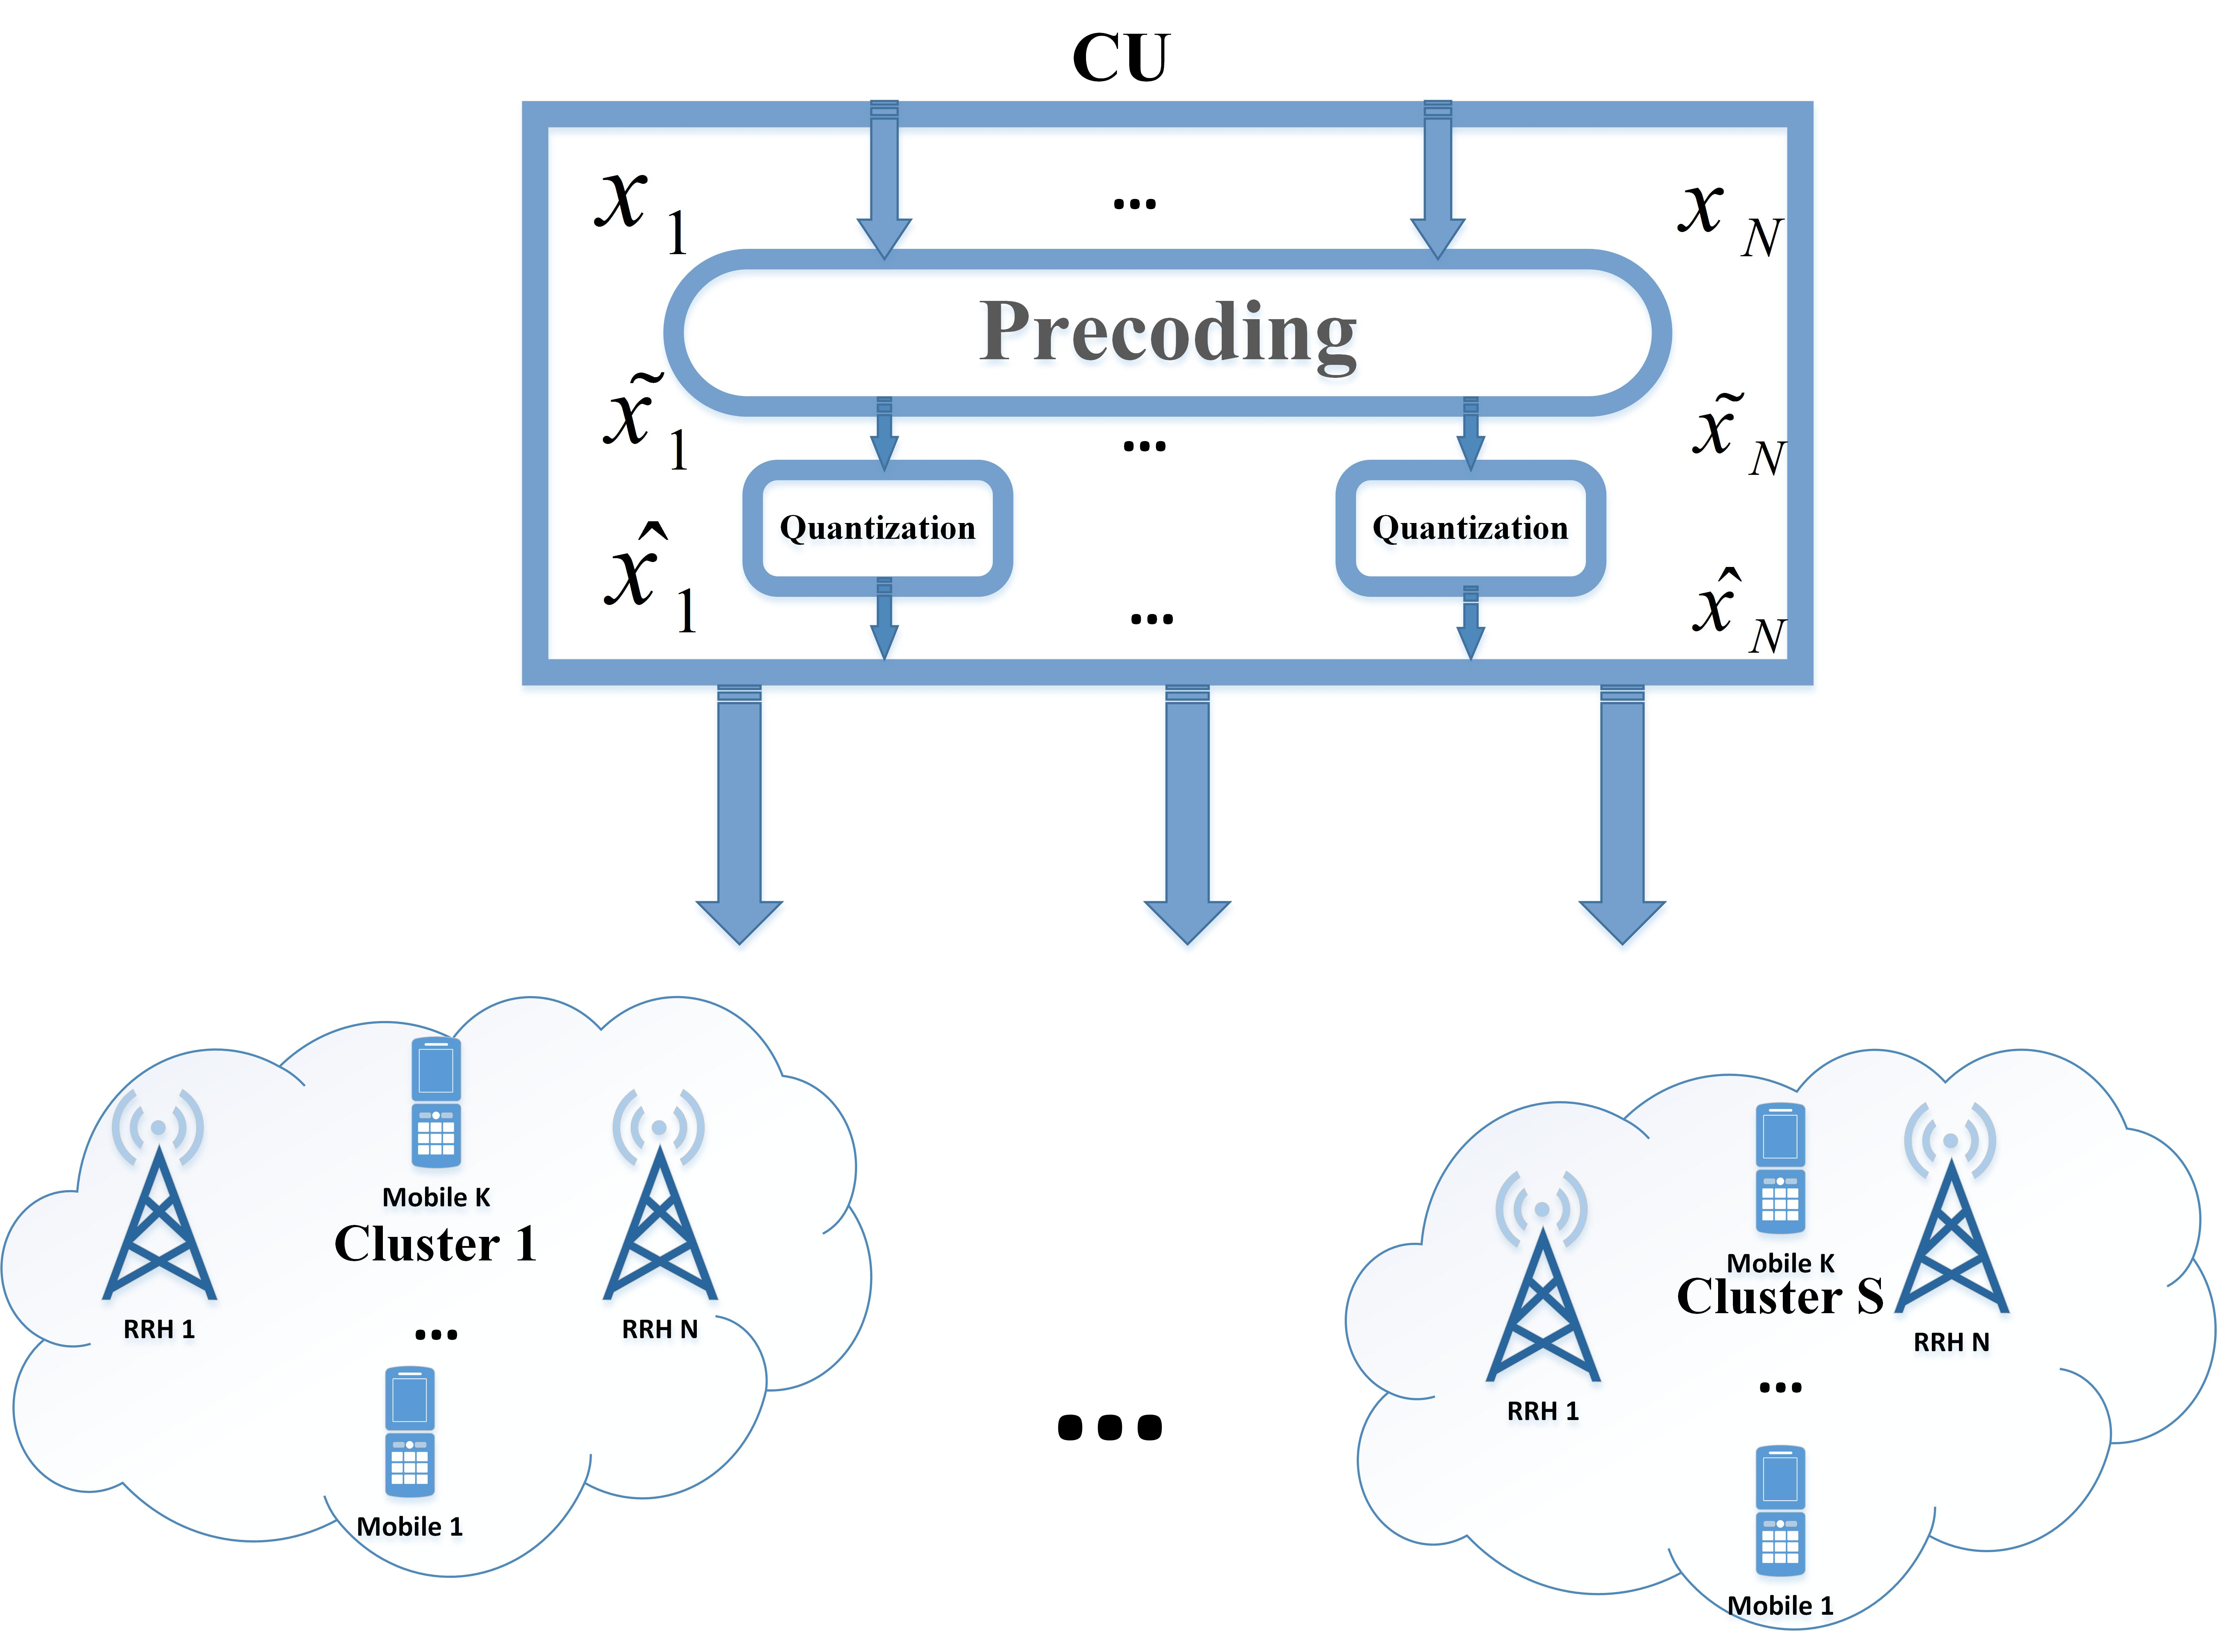
\includegraphics[width=\linewidth]{./fig/mydraw1}
  \caption{ساختار 
  \lr{C-RAN}
  در  لینک فروسو.
  }
  \label{fig:cr1}
\end{figure}
 فرض مسئله بر این است که سیستم به صورت چند آنتنه (\lr{MIMO})  می باشد و ظرفیت \lr{Fronthaul} محدود است. همچنین، سیستم دارای چندین خوشه یا سلول که در هر خوشه، تعدادی  واحد رادیویی و تعدادی کاربر قرار دارد\cite{EEcluster,jcluster}. هدف، بدست آوردن بیشینه بازدهی انرژی می باشد.\newline
 در حالت لینک فروسو، پیام، پیش کدگذاری شده است و سپس فشرده سازی بر روی آن صورت گرفته است و از طریق لینک \lr{Fronthaul} به واحد رادیویی منتقل می شود تا پیام را به کاربران ارسال کنند \cite{Fronthaul, ulSimeone, precodSimeone}
 .\newline
 در حالت لینک فراسو، سیگنال از کاربران به واحدهای رادیویی منتقل شده و سپس پیام فشرده شده و به دست واحد کنترل می رسد؛ تا با استفاده از روش های ترکیب کردن \LTRfootnote{combining}، پیام ارسالی کاربران بازیابی شود. 

\section{لینک فروسو}
در این بخش، لینک فروسو برای سیستم \lr{MIMO C-RAN} در نظر گرفته شده است که واحد کنترل، پیام را پیش کدگذاری کرده سپس سیگنال پیش کدگذاری شده را فشرده می کند. سیگنال فشرده شده ی نهایی توسط لینک \lr{Fronthaul} با ظرفیت محدود منتقل می گردد
\cite{dlsnr}.
\newline
فرض بر این است که واحدهای رادیویی و کاربران خوشه بندی شده اند به طوری که در هر خوشه تعدادی واحد رادیویی است که به کاربران موجود در آن خوشه، سرویس دهی می کنند.\newline
در این سیستم، فرستنده می بایست اطلاعات حالت کانال را بداند
(\lr{CSIT}). 
 از آنجایی که \lr{CSIT} با کمی خطا با ارسال پایلوت در لینک فراسو بدست می آید، به همین دلیل فرض در اینجا به این صورت است که تخمین \lr{CSIT}، همراه با خطای مشخص است. در واحد کنترل، از پیش کدگذاری از نوع \lr{MMSE} برای کاهش تداخل بین کاربران و بهبود عملکرد سیستم استفاده می گردد.\newline
همچنین، ابتدا نرخ قابل دسترسی را با توجه به ظرفیت محدود \lr{Fronthaul}، بدست می آوریم. سپس توان تخصیص داده را بهینه می کنیم تا \lr{EE} به مقدار بهینه ی خود برسد.\newline
در ادامه، ابتدا مدل سیستم و سپس نرخ قابل دسترسی بیان شده و مسئله ی تخصیص توان بررسی می گردد\cite{mkm}.
\subsection{مدل سیستم}
لینک فروسو سیستم \lr{MIMO C-RAN} شامل $R$  واحد رادیویی می باشد که $D$ کاربر تک آنتنه را سرویس می دهند.فرض بر این است که کاربران و واحدهای رادیویی، به 
 $S$
 تا خوشه تقسیم شده اند که $v$ امین خوشه،
 دارای $R_v$ واحد رادیویی است که ${D}_v$ کاربر را سرویس دهی می کنند\cite{EEcluster}.
 همچنین، فرض بر این است که
$j$
امین واحد رادیویی، در $v$امین خوشه، توسط لینک فیبر نوری با ظرفیت محدود $c_{r_{(v,j)}}$ به \lr{CU} متصل می گردد. در نتیجه داریم:
\begin{equation}
\begin{split}
\mathcal{R}_v= \{  r_{(v,i)} | 1 \leq i \leq {R}_v , i\in Z^+\}, \\
\mathcal{C}_{\mathcal{R}_v}= \{C_{r_{(v,j)}}| 1 \leq j \leq {R}_v , j\in Z^+\}, \\
\mathcal{D}_v= \{  d_{(v,k)} | 1 \leq k \leq {D}_v , k\in Z^+\},  \\
\end{split}
\end{equation} 
که
 $\mathcal{R}_v$، $\mathcal{C}_{\mathcal{R}_v}$
 و
  $\mathcal{D}_v$
 به ترتیب نشان دهنده ی دسته ی واحدهای رادیویی، دسته ی ظرفیت لینک \lr{Fronthaul} و دسته ی کاربران در $v$امین دسته ی خوشه می باشد.\newline
در واحد کنترل، ما روش فشرده سازی بعد از پیش کدگذاری و سپس ارسال را اعمال کرده ایم. هر کاربر همزمان تداخل بین خوشه ها و داخل یک خوشه را همزمان دریافت می کنند.
 \subsection{آنالیز نرخ قابل دسترس}
در این زیربخش، نرخ قابل دسترسی سیستم بررسی می گردد.
\begin{theorem}\label{t1}
 نرخ قابل دسترسی برای کاربر $d_{(s,k)}$ به صورت زیر می باشد:
\begin{equation}\label{e1}
\mathfrak{R}_{d_{(s,k)}} = B \log_2(1+\gamma_{d_{(s,k)}}),
\end{equation}
که $B$ پهنای باند کانال و $\gamma_{d_{(s,k)}}$ همان \lr{SINR} دریافتی $k$امین کاربر در $s$امین دسته ی خوشه است که به صورت زیر بیان می گردد.  
\begin{equation}\label{5}
\gamma_{d_{(s,k)}}= \frac{p_{d_{(s,k)}}|\boldsymbol{h}_{\mathcal{R}_s, d_{(s,k)}}^H \boldsymbol{w}_{\mathcal{R}_{s},d_{(s,k)}}|^2}{I_{d_{(s,k)}}+BN_0}.
\end{equation}
در فرمول \eqref{5}، 
$I_{d_{(s,k)}}$
نشان دهنده ی توان سیگنال تداخلی است.$BN_0$
نشان دهنده ی توان نویز است و
$\boldsymbol{h}_{\mathcal{R}_s, d_{(s,k)}}$ 
 نشان دهنده ی بردار کانال بین $k$امین کاربر و واحدهای رادیویی
 $s$
 امین دسته ی خوشه می باشد. همچنین 
 $\boldsymbol{w}_{\mathcal{R}_{s},d_{(s,k)}}$
 نشان دهنده ی بردار پیش کدگذاری استفاده شده در $s$امین دسته ی خوشه ها برای $k$امین کاربر می باشد. 
 $p_{d_{(s,k)}}$
 توان ارسالی واحدهای رادیویی است که به $k$امین کاربر در $s$امین دسته ی خوشه ارسال می گردد.
\end{theorem}
\begin{proof}
فرض کنید $\boldsymbol{y}_{\mathcal{D}_s}$ یک بردار
 $D_s \times 1$
باشد که نشان دهنده ی سیگنال دریافتی توسط دسته ای از کاربران در $s$
امین خوشه باشد که به صورت زیر بدست می آید.
\begin{equation} \label{1}
\boldsymbol{y}_{\mathcal{D}_s} = \sum_{v=1}^S \boldsymbol{H}^H_{\mathcal{R}_v,\mathcal{D}_s}\hat{\boldsymbol{x}}_{\mathcal{R}_v}+ \boldsymbol{z}_{\mathcal{D}_s},
\end{equation}
که   $\hat{\boldsymbol{x}}_{ \mathcal{R}_v} = [\hat{x}_{ r_{(v,1)}},...,\hat{ x}_{ r_{(v,\mathcal{R}_v)}}]^T \in \mathbb{C}^{{R}_v } $ 
بردار سمبل ارسالی خوشه ی  $v$ ام می باشد.\newline
 $\boldsymbol{z_{\mathcal{D}_s}} \backsim \mathcal{N}(0,N_0\boldsymbol{I}_{{D}_s})$ 
 نویز گوسی سفید اضافه شونده می باشد که دارای توان $N_0$
 و 
 $\boldsymbol{H}_{\mathcal{R}_v,\mathcal{D}_s}=\left[\boldsymbol{h}_{\mathcal{R}_v,d_{(s,1)}},\ldots,\boldsymbol{h}_{\mathcal{R}_v,d_{(s,\mathcal{D}_s)}}\right]^T  \in \mathbb{C}^{{R}_v\times {D}_s}$ 
 نشان دهنده ی ماتریس کانال بین واحدهای رادیویی دسته ی $\mathcal{R}_v$ و کاربران $\mathcal{D}_s$ می باشد.
 بردار کانال از واحدهای رادیویی خوشه ی  $v$ به $k$ امین کاربر در خوشه ی $s$ام  
 $\boldsymbol{h}_{\mathcal{R}_v,d_{(s,k)}}\in \mathbb{C}^{{R}_v}$
 به صورت زیر مدل می شود \cite{cellfree}
 \begin{equation}\label{channel}
\boldsymbol{h}_{\mathcal{R}_v,d_{(s,k)}} = \boldsymbol{\beta}^\frac{1}{2}_{\mathcal{R}_v,d_{(s,k)}} \boldsymbol{g}_{\mathcal{R}_v,d_{(s,k)}},
\end{equation}
% resizebox{0.3\hsize}{!}{$
که  $\boldsymbol{g}_{\mathcal{R}_v,d_{(s,k)}} \backsim \mathcal{N}(0,N_0\boldsymbol{I}_{\mathcal{D}_s})$ نشان دهنده ی بردار کانال محو شدگی سریع و مسطح می باشد 
و $\boldsymbol{\beta}_{\mathcal{R}_v,d_{(s,k)}}=\text{\lr{diag}}(a_{r_{(v,1),d_{(s,k)}}},\ldots,a_{r_{(v,\mathcal{R}_v),d_{(s,k)}}})$
نشان دهنده ی محوشدگی  در مقیاس بزرگ می باشد. همچنین سیگنال ارسالی تحت فشرده سازی به صورت زیر است
\begin{equation}
\label{eq_pow1}
 \hat{\boldsymbol{x}}_{\mathcal{R}_v} = \tilde{\boldsymbol{x}}_{\mathcal{R}_v} + \boldsymbol{Q}_{\mathcal{R}_v},
\end{equation}

که در اینجا $\boldsymbol{Q}_{\mathcal{R}_v} = \left[ q_{r_{(v,1)}},\ldots,q_{r_{(v,R_v)}}\right]^T$ نشان دهنده ی بردار نویز کوانتیزاسیون می باشد که به دلیل فشرده سازی بعد از پیش کدگذاری در واحد کنترل ایجاد می گردد که دارای توزیع $q_{M_{(t,i)}}\backsim \mathcal{N}(0,\sigma_{q_{(t,i)}}^2) $ است.
علاوه بر این،  
$$\tilde{\boldsymbol{x}}_{\mathcal{R}_v} = \textbf{\lr{W}}_{\mathcal{R}_v,\mathcal{D}_v} \textbf{\lr{P}}_{\mathcal{D}_v}^{\frac{1}{2}} \boldsymbol{x}_{ \mathcal{D}_v},$$
نشان دهنده ی پیام پیش کدگذاری شده قبل از فشرده سازی می باشد.
همانطور که گفته شده بود، فرض بر این است که بردار کانال را می دانیم و همراه با خطا بدست آمده است؛ کانال همراه با خطا به صورت زیر مدل شده است: 
\begin{equation*}
\hat{\boldsymbol{h}}_{\mathcal{R}_v,d_{(s,k)}} = \boldsymbol{h}_{\mathcal{R}_v,d_{(s,k)}} + \Delta \boldsymbol{h}_{\mathcal{R}_v,d_{(s,k)}},
\end{equation*}

$\Delta \boldsymbol{h}_{\mathcal{R}_v,d_{(s,k)}}$
نشان دهنده ی بردار خطای تخمین زده شده است که دارای توزیع گوسی به صورت
$$\Delta \boldsymbol{h}_{\mathcal{R}_v,d_{(s,k)}}\backsim \mathcal{N}(0,\boldsymbol{\phi}_{\mathcal{R}_v,d_{(s,k)}}^2),$$
است که  داریم 
$$\boldsymbol{\phi}_{\mathcal{R}_v,d_{(s,k)}} = \text{\lr{diag}}(\phi_{r_{(v,1)},d_{(s,k)}},\ldots,\phi_{r_{(v,\mathcal{R}_v)},d_{(s,k)}}).$$
با استفاده از پیش کدگذاری \lr{MMSE}، ماتریس پیش کدگذاری به صورت زیر است \cite{digCom}
\begin{equation}
\boldsymbol{W}_{\mathcal{R}_s,\mathcal{D}_s} = \hat{\boldsymbol{H}}_{\mathcal{R}_s,\mathcal{D}_s}(\hat{\boldsymbol{H}}_{\mathcal{R}_s,\mathcal{D}_s}^H \hat{\boldsymbol{H}}_{\mathcal{R}_s,\mathcal{D}_s}+ \alpha \boldsymbol{I}_{{D}_s})^{-1},
\end{equation} 
همچنین  $\alpha$، فاکتور رگولاریزاسیون است
بنابراین، $I_{d_{(s,k)}}$ را که توان تداخلی بر روی کاربر بود به صورت زیر می توان تخمین زد.
\begin{equation}\label{6}
\begin{split}
I_{d_{(s,k)}} &=  \underbrace{\sum_{\substack{l=1 \\ l\neq k}}^{{D}_s} |\boldsymbol{h}_{\mathcal{R}_s, d_{(s,k)}}^H \boldsymbol{w}_{\mathcal{R}_{s},d_{(s,l)}}|^2  p_{d_{(s,l)}}}_{\text{(\lr{intra-cluster interference})}}\\
&+\underbrace{\sum_{\substack{v=1 \\ v\neq s}}^{S} \sum_{l=1}^{{D}_v} |\boldsymbol{h}_{\mathcal{R}_v, d_{(s,k)}}^H \boldsymbol{w}_{\mathcal{R}_{v},d_{(v,l)}}|^2 p_{d_{(v,l)}}}_{\text{(\lr{inter-cluster interference})}}\\
& +\underbrace{ \sum_{v=1}^{S} \sum_{i=1}^{{R}_v} {\sigma_q}_{r_{(v,i)}}^2  |h_{r_{(v,i)}, d_{(s,k)}}|^2 }_{\text{(\lr{quantization noise interference})}}.
\end{split}
\end{equation}
\end{proof}
\subsection{بهینه سازی تخصیص توان}
می دانیم که توان سیگنال ارسالی توسط  $i$امین واحد رادیویی در $s$امین خوشه  به صورت زیر می باشد : 
\begin{equation} \label{eq_pow2}
\bar{p}_{r_{(s,i)}} = \mathit{E}[|| \hat{x}_{\mathcal{D}_v} ||^2],
\end{equation}

با قرار دادن رابطه ی  (\ref{eq_pow1}) در (\ref{eq_pow2})، توان سیگنال ارسالی به این صورت بدست می آید:
\begin{equation}
\bar{p}_{r_{(s,i)}} = \boldsymbol{w}_{r_{(s,i)},\mathcal{D}_{s}} \boldsymbol{P}_{\mathcal{D}_s}^{\frac{1}{2}} \boldsymbol{P}_{\mathcal{D}_s}^{H \frac{1}{2}}   \boldsymbol{w}_{r_{(s,i)},\mathcal{D}_{s}}^H + \sigma_{q_{(s,i)}}^2.
\end{equation}
در نتیجه نرخ قابل دسترس بر روی لینک \lr{fronthaul}، بین واحد کنترل و $i$امین واحد رادیویی در $t$امین خوشه  به صورت زیر بدست می آید 
\begin{equation}
C_{r_{(t,i)}} = \log{(1+\frac{\boldsymbol{w}_{r_{(s,i)},\mathcal{D}_{s}} \boldsymbol{P}_{\mathcal{D}_s}^{\frac{1}{2}} \boldsymbol{P}_{\mathcal{D}_s}^{H \frac{1}{2}}   \boldsymbol{w}_{r_{(s,i)},\mathcal{D}_{s}}^H }{ \sigma_{q_{(s,i)}}^2})},
\end{equation}
\subsubsection{شرح مسئله}
نسبت مجموع نرخ ها در سیستم به کل توان ارسالی واحدهای رادیویی نشان دهنده ی بازدهی انرژی است که یکی از مهم ترین پارامترها در انتخاب تکنولوژی می باشد که با $\eta$ نمایش داده می شود و می توان اینگونه بیان کرد
\begin{equation}\label{eta}
\eta(\boldsymbol{P}) := \frac{\sum\limits_{s=1}^{S} \sum\limits_{k=1}^{{D}_s}\mathfrak{R}_{d_{(s,k)}} }{\sum\limits_{s=1}^{S} \sum\limits_{i=1}^{{R}_s}\bar{p}_{r_{(s,i)}}} = \frac{R_{total}(\boldsymbol{P})}{P_{RRH}(\boldsymbol{P})},
\end{equation}
که در اینجا  $ \boldsymbol{P} = \{ \boldsymbol{P}_{\mathcal{D}_s}|  1 \leq s \leq S, s \in \mathbb{Z}^{+} \}$ ماتریس تخصیص توان است. در این بخش، بیشینه سازی بازدهی انرژی با شروط زیر مورد بررسی قرار می گیرد 
\begin{equation}\label{p1}
\begin{aligned}
\max\limits_{\boldsymbol{P}}   \quad &   \eta(\boldsymbol{P})\\
\text{\lr{subject to}} \quad  & \bar{p}_{r_{(s,i)}} \leq P_{max} && \qquad \forall s, \forall i,   \\
&\mathfrak{R}_{d_{(s,k)}} \geq  \mathfrak{R}_{d_{(s,k)}}^{th} && \qquad \forall s, \forall k, \\
&C_{r_{(s,i)}} \leq C_{r_{(s,i)}}^{th}  &&\qquad \forall s, \forall i, \\
&p_{d_{(s,k)}}  \geq 0                                  &&\qquad \forall s, \forall k, \\
\end{aligned}			
\end{equation}
از آنجایی که این یک مسئله ی محدب نیست، با روش الگوریتم تکرار شونده ، مقدار توان بهینه را بدست می آوریم\cite{boyd}.
\subsection{روش مورد استفاده}
در این قسمت، به جای ماکسیمم کردن \eqref{eta}، مسئله ی معادل آن را با الگوریتم تکرار شونده حل می کنیم
\begin{theorem}\label{t2}
مقدار ماکسیمم $\eta^*$  تنها زمانی بدست می آید که
\begin{equation}\label{q2}
\begin{split}
&\max \limits_{\boldsymbol{P}} (R_{total}(\boldsymbol{P}) - \eta^* P_{RRH}(\boldsymbol{P}))=\\
& R_{total}(\boldsymbol{P}^*) - \eta^* P_{RRH}(\boldsymbol{P}^*) =0,
\end{split}
\end{equation}
که $\{\boldsymbol{P}\}$  یک پاسخ امکان پذیر برای مسئله ی \eqref{p1} باشد \cite{hcranEE}.
\end{theorem}
\begin{proof}
اثبات این قضیه با روش مشابه در مقاله ی \cite{hcranEE} حل شده است.
\end{proof}

برای حل مسئله ی بهینه سازی \eqref{q2}، از تابع لاگرانژ استفاده می کنیم \cite{boyd} که توسط الگوریتم تکرار شونده بدست می آید. برای ساده سازی کران بالا برای تداخل  \eqref{6}، به این صورت بدست می آید
\begin{equation}
\begin{split}
\tilde{I}_{d_{(s,k)}} &= \sum_{v=1}^{S} P_{max}|| \boldsymbol{h}_{\mathcal{R}_v,d_{(s,k)}} \boldsymbol{w}_{\mathcal{R}_v,d_{(s,k)}}||^2 ,\\
& +  \sum_{v=1}^{S} \sum_{i=1}^{{R}_v} {\sigma_q}_{r_{(v,i)}}^2  |h_{r_{(v,i)}, d_{(s,k)}}|^2.
\end{split}
\end{equation}
بنابراین، برای بدست آوردن توان بهینه کران پایینی برای نرخ بدست می آید
\begin{equation}\label{e11}
\mathfrak{\tilde{R}}_{d_{(s,k)}} = B \log_2(1+\tilde{\gamma}_{d_{(s,k)}}),
\end{equation}
که  $\tilde{\gamma}_{d_{(s,k)}}$ به صورت زیر است 
\begin{equation}\label{15}
\tilde{\gamma}_{d_{(s,k)}} =  \frac{p_{d_{(s,k)}}|\boldsymbol{h}_{\mathcal{R}_s, d_{(s,k)}}^H \boldsymbol{w}_{R_{s},d_{(s,k)}}|^2}{\tilde{I}_{d_{(s,k)}}+BN_0};
\end{equation}

همانطور که قبلا بیان شد، الگوریتم تکرار شونده برای بهینه سازی مورد استفاده قرار می گیرد که براساس ضرایب تابع لاگرانژ می باشد 
\begin{equation}
\begin{split}
\mathcal{L}(\boldsymbol{P}; \boldsymbol{\lambda}, \boldsymbol{\mu}, \boldsymbol{ \kappa}) & = \sum\limits_{s=1}^{S} \sum\limits_{k=1}^{\mathcal{D}_s}\mathfrak{\tilde{R}}_{d_{(s,k)}} 
- \eta \sum\limits_{s=1}^{S} \sum\limits_{i=1}^{\mathcal{R}_s}\bar{p}_{r_{(s,i)}}\\
&+\sum\limits_{s=1}^{S} \sum\limits_{k=1}^{\mathcal{D}_s} \lambda_{d_{(s,k)}} (\mathfrak{\tilde{R}}_{d_{(s,k)}}-\mathfrak{R}_{d_{(s,k)}}^{th})\\
&- \sum\limits_{s=1}^{S} \sum\limits_{i=1}^{\mathcal{R}_s} \mu_{r_{(s,i)}} (\bar{p}_{r_{(s,i)}}-P_{max})\\
&- \sum\limits_{s=1}^{S} \sum\limits_{i=1}^{\mathcal{R}_s} \kappa_{r_{(s,i)}} (C_{r_{(s,i)}}-C_{r_{(s,i)}}^{th}).\\
\end{split}
\end{equation}
که در اینجا، $\boldsymbol{\lambda}, \boldsymbol{\mu}, \boldsymbol{\kappa} \geq 0$
بردارهای ضرایب لاگرانژ می باشد .\newline
با استفاده از این معادله، توان بهینه به صورت زیر بدست می آید
\begin{equation}
p_{d_{(s,k)}}^* =[\frac{ B(1+\lambda_{d_{(s,k)}} )}{\ln2 \times (\iota_{d_{(s,k)}}+ \chi_{d_{(s,k)}})} -\frac{\tilde{I}_{d_{(s,k)}} + BN_0}{\nu_{d_{(s,k)}} }]^+;
\end{equation} 
که داریم
 $$\nu_{d_{(s,k)}} =|h_{\mathcal{R}_s, d_{(s,k)}}^H \boldsymbol{w}_{R_{s},d_{(s,k)}}|^2,$$
 $$\iota_{d_{(s,k)}}= \sum\limits_{i=1}^{\mathcal{R}_s} (\mu_{r_{(s,i)}}+\eta)(w_{r_{(s,i)},d_{(s,k)}} w_{r_{(s,i)},d_{(s,k)}}^*),$$
 $$\chi_{r_{(s,i)}} \approx  \sum\limits_{i=1}^{\mathcal{R}_s} \frac{\kappa_{r_{(s,i)}}}{\ln 2}\frac{(w_{r_{(s,i)},d_{(s,k)}} w_{r_{(s,i)},d_{(s,k)}}^*)}{ P_{max}}.$$
  در آخر، برای بدست آوردن توان بهینه، الگوریتم \eqref{alg} مورد استفاده قرار می گیرد \cite{hcranEE}
 \begin{latin}
\begin{algorithm}
\caption{Energy-Efficient Power Allocation}\label{alg}
\begin{algorithmic}

\State Set the maximum number of iterations $I_{max}$, convergence condition $\epsilon_{\eta}$  and the initial value $\eta^{(1)} = 0$
\State Set the iteration index $i = 1$ and begin the iteration (Outer
Loop).
\For {$ 1\leq i \leq  Imax$}
\State Solve the resource allocation problem with $\eta^{(i)}$ (Inner Loop);
\State Obtain $P^{(i)}, R_{total}^{(i)}, P_{RRH}^{(i)}$
\If {$ R_{total}(\boldsymbol{P}^{(i)}) - \eta^{(i)} P_{RRH}(\boldsymbol{P}^{(i)}) < \epsilon_{\eta} $} 
\State Set $\boldsymbol{P}^*= \boldsymbol{P}^{(i)} $   and  $ \eta^{*} =\eta^{(i)} $;
\State break;
\Else
\State Set $\eta^{(i)}= \frac{R_{total}(\boldsymbol{P}^{(i))}}{P_{RRH}(\boldsymbol{P}^{(i))}}$ and $i= i+1$;
\EndIf 
\State \textbf{end if}
\EndFor 
\State \textbf{end for}

\end{algorithmic}
\end{algorithm}
\end{latin}
%%%%%%%%%%%%%%%%%%%%%%%%%%%%%
\subsection{نتایج عددی}
در این بخش، نتایج عددی الگوریتم مورد استفاده برای سیستم \lr{MIMO C-RAN} با پارامترهای بیان شده در جدول \ref{tab:title} بیان می شود.
\begin{latin} 
 \begin{table}[H]
 \caption {\rl{پارامترهای شبیه سازی}} \label{tab:title} 
 \begin{center}
  \begin{tabular}{||c c ||} 
  \hline
  Parameter & Value \\ [0.5ex] 
  \hline\hline
  Number of cluster S & 2 \\ 
  \hline
  Noise power density & -174dBm/Hz\\
  \hline
  Bandwidth & 120KHz \\
  \hline
 Maxmimun transmit Power & 23dBm \\
  \hline
  Circuit Power of whole RRHs & 10dBm \\
  \hline
  Variance of quantization noise & $10^{-4}$ \\
  \hline
   Maxmimun fronthaul link's rate & 5bits/sec/Hz \\
  \hline
  Minimum data rate &  1bits/sec/Hz \\ [1ex] 
  \hline
 \end{tabular}
 \end{center}
 \end{table}
 \end{latin}
  \begin{figure}[h]
  \centering
    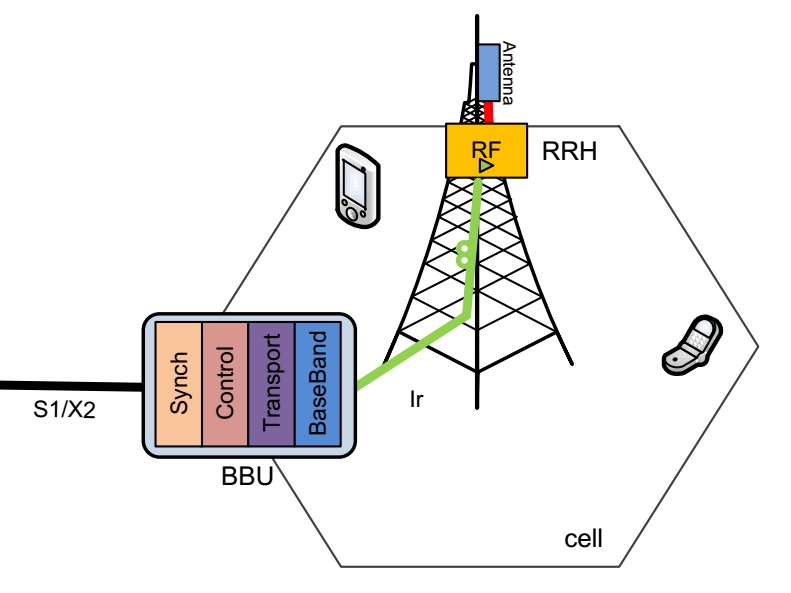
\includegraphics[width=\linewidth, height=12cm]{./fig3/rrh}
  \caption{
  بازدهی انرژی با توجه به تغییرات تعداد واحدهای رادیویی در هر خوشه برای توان بهینه برای 
   دو کاربر مختلف
   و پارامترهای جدول \ref{tab:title}}
  \label{fig:nem1}
\end{figure}
 در شکل \ref{fig:nem1}، بازدهی انرژی سیستم \lr{MIMO C-RAN} بر اساس تعداد واحدهای رادیویی در هر خوشه برای الگوریتم مورد استفاده و برای دو تعداد کاربر متفاوت، رسم شده است. 
 همانطور که  شکل  نشان می دهد، با افزایش تعداد واحدهای رادیوی، بازدهی انرژی افزایش می یابد و سپس  در این شکل از حدود 50 واحد رادیویی شیب افزایش بازدهی انرژی کمتر شده و به نظر می آید که رو به ثابت شدن است زیرا با افزایش واحد های رادیویی ابتدا نرخ ارسال داده بیشتر می شود و بازدهی انرژی بهبود می یابد و در نهایت نرخ ارسال داده دیگر بیشتر نمی گردد و ثابت می شود. زیرا در اینجا با افزایش تعداد واحدهای رادیویی، مجموع توان کل افزایش می یابد در نتیجه نرخ انتقال داده نیز بیشتر می گردد.

  \begin{figure}[h]
  \centering
    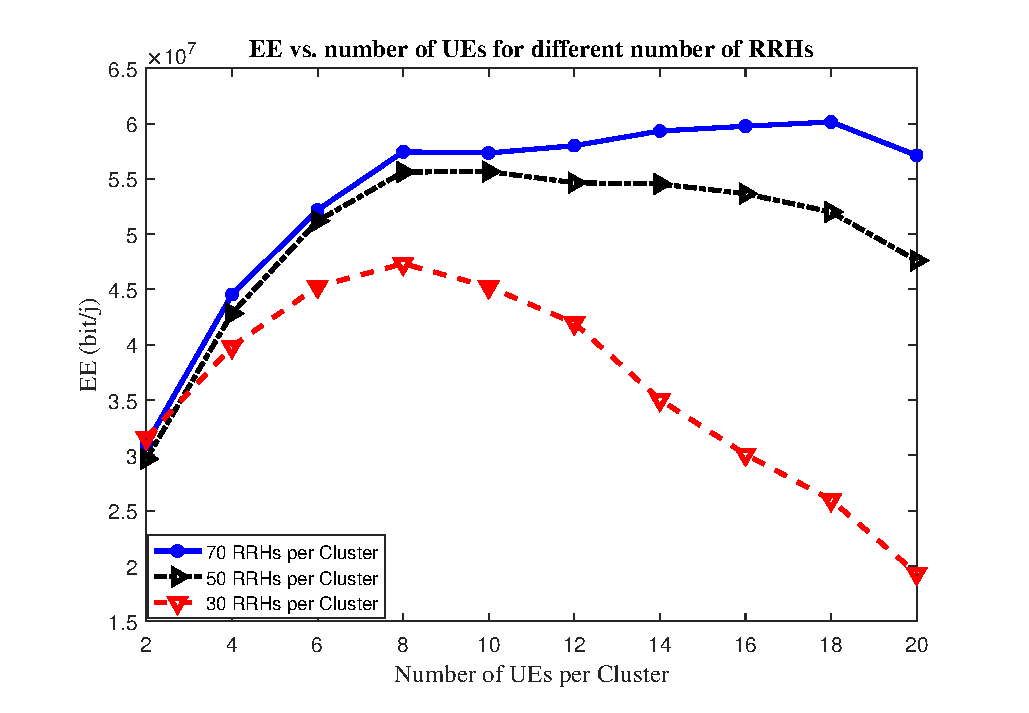
\includegraphics[width=\linewidth]{./fig3/ueEnd}
  \caption{  بازدهی انرژی با توجه به تغییرات تعداد کاربران در هر خوشه برای توان بهینه  برای 
   سه واحد رادیویی مختلف
   و پارامترهای جدول \ref{tab:title} و $P_c = 9dbm$}
  \label{fig:nem2}
\end{figure}


در شکل \ref{fig:nem2}، بازدهی انرژی بر اساس تعداد کاربران در هر خوشه برای الگوریتم مورد استفاده و برای سه تعداد واحد رادیویی متفاوت، رسم شده است.همانطور که  دیده می شود با افزایش تعداد کاربران، ابتدا شیب نمودار زیاد می شود و بازدهی انرژی افزایش می یابد زیرا با افزایش کاربران مجموع نرخ های انتقال افزایش می یابد ولی از یک مقدار به بعد تداخل بین کاربران افزایش می یابد و تاثیر خودر را به طور محسوس بر بازدهی انرژی می گذارد و در نتیجه بازدهی انرژی کاهش می یابد. 

%\bibliographystyle{ieeetr}
%\bibliography{bib1}
%\setLTRbibitems
\begin{figure}[H]
  \centering
    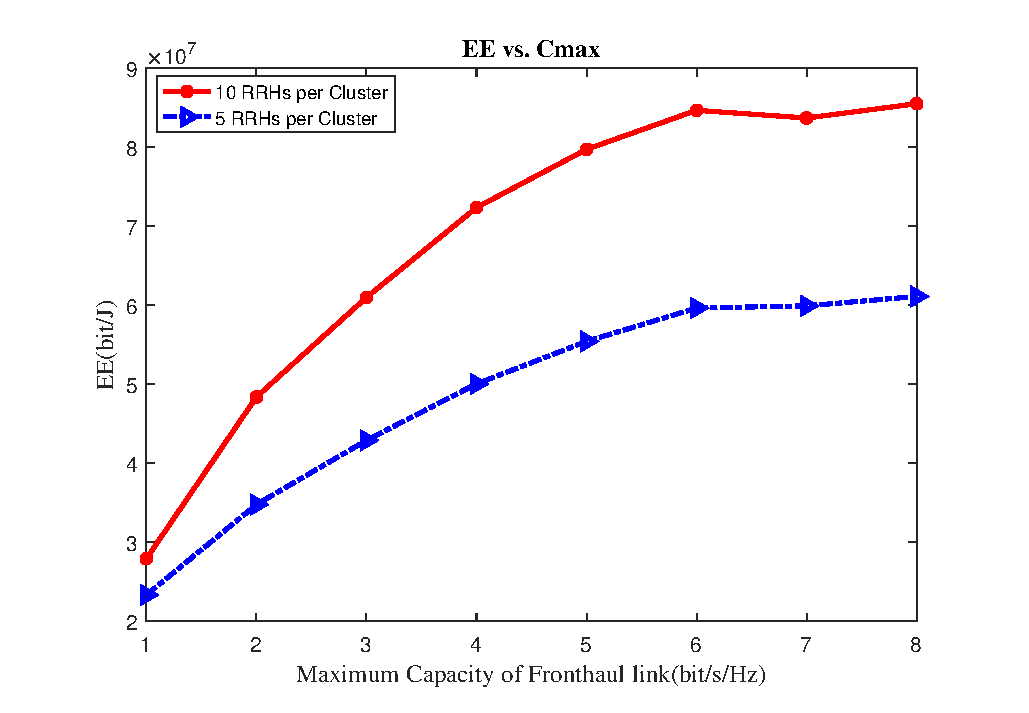
\includegraphics[width=\linewidth]{./fig3/cm}
  \caption{  بازدهی انرژی با توجه به تغییرات $C^{th}$، در در حالت $S =2$, $\text{\lr{Number of RRHs per Cluster}} = 10 , 5$, $\text{\lr{Number of UE per Cluster}} =2$ }
  \label{fig:nem3}
\end{figure}

در شکل \ref{fig:nem3}، بازدهی انرژی بر اساس محدودیت ظرفیت لینک \lr{fronthaul}، برای دو تعداد متفاوت  5 و 10 واحد رادیویی در هر خوشه رسم شده است. با توجه به شکل، زمانی که ظرفیت یک مقداری بیشتر
 می گردد، بدلیل اینکه نرخ قابل دسترس توسط تعداد کاربران و واحدهای رادیویی محدود می گردد، به نظر می آید افزایش محدودیت این ظرفیت تاثیر چندانی در بازدهی انرژی ندارد.  

% \begin{figure}[H]
%  \centering
%    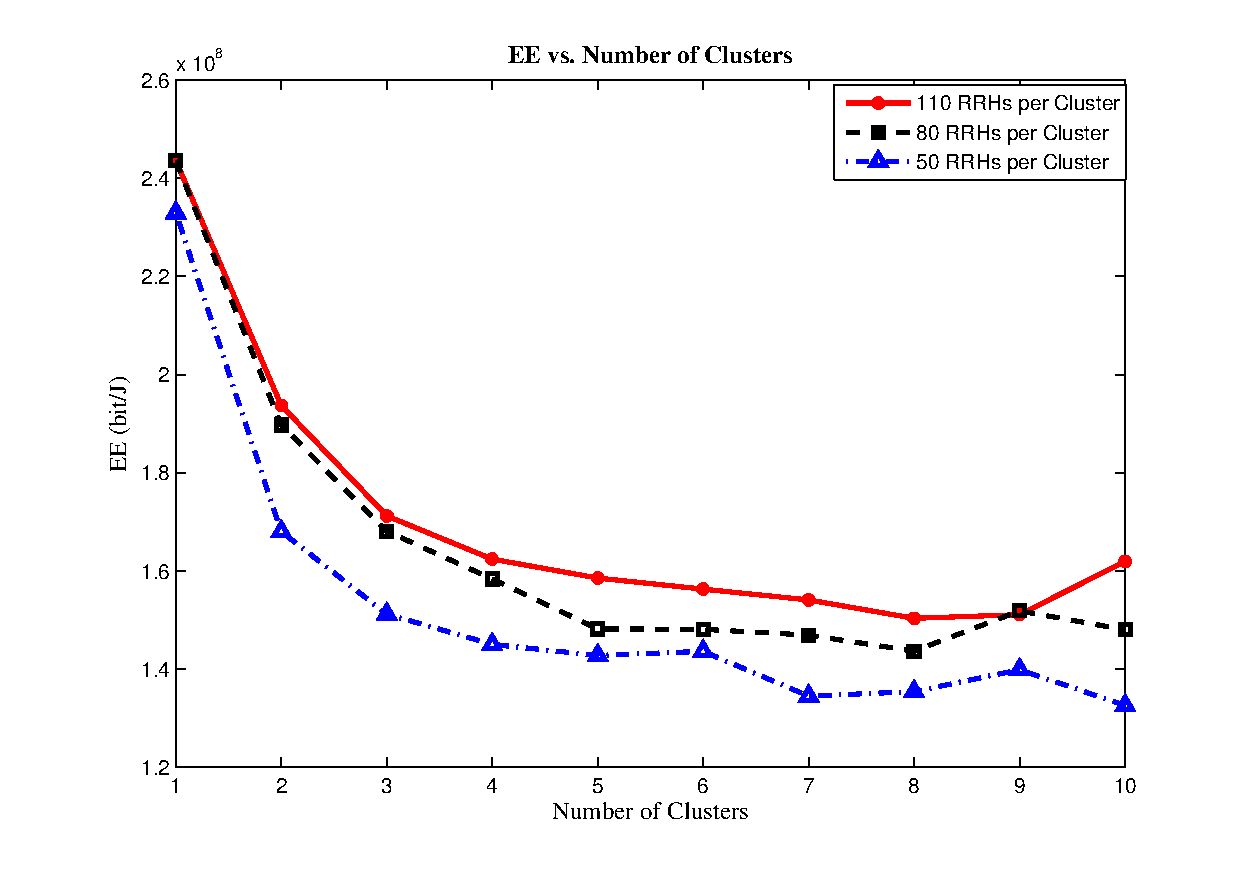
\includegraphics[width=\linewidth]{./fig3/clust}
%  \caption{  بازدهی انرژی بر حسب تعداد خوشه ها برای سه مقدار 50 و 80 و 110 واحد رادیویی}
%  \label{fig:cluster}
%\end{figure}
% حال در شکل \ref{fig:cluster}، بازدهی انرژی بر حسب تعداد خوشه ها برای سه مقدار 50 و 80 و 110 واحد رادیویی در هر خوشه با فرض وجود 3 کاربر در هر خوشه رسم شده است. همانطور که می بینید با افزایش خوشه ها بازدهی انرژی کاهش یافته است.
% 
 
 \begin{figure}[H]
  \centering
    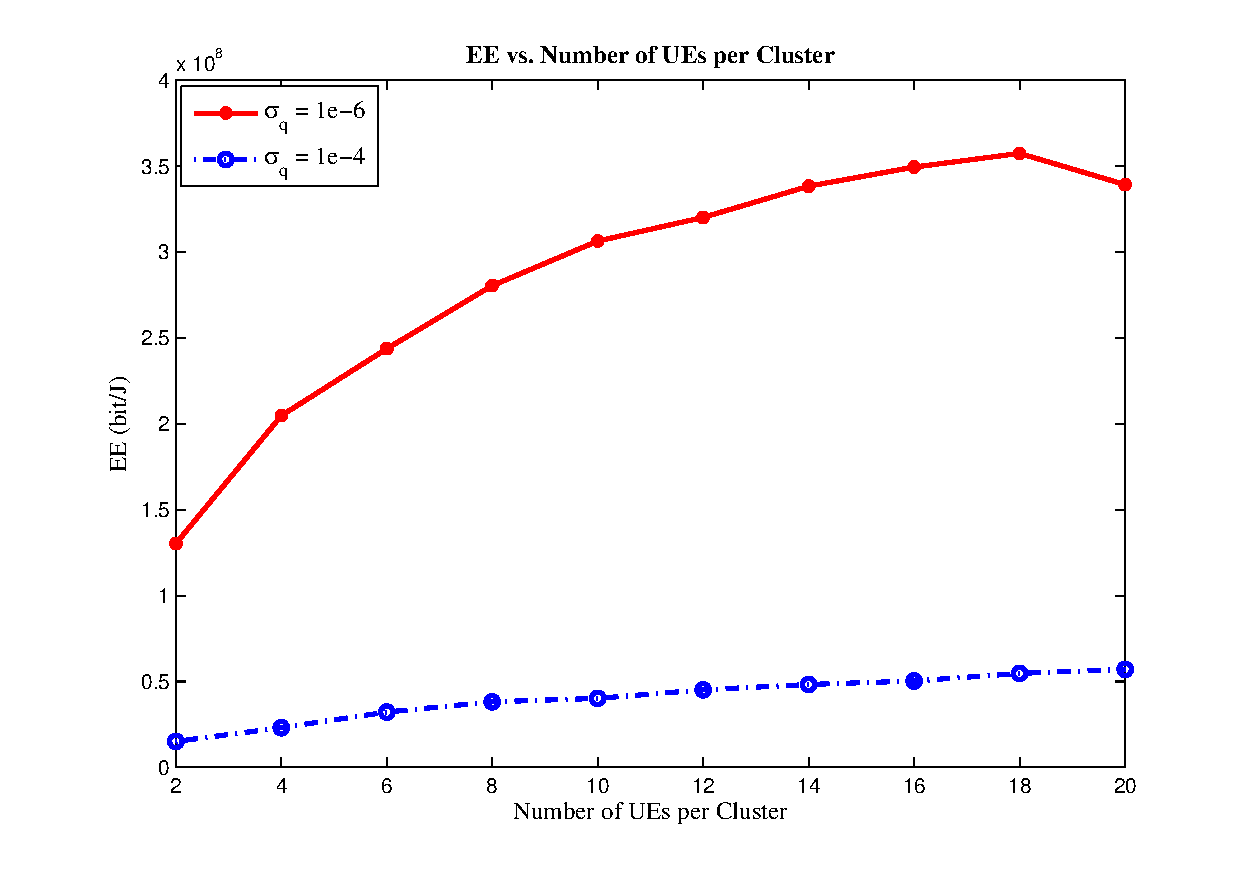
\includegraphics[width=\linewidth]{./fig3/varUE}
  \caption{  بازدهی انرژی بر حسب تعداد کاربران در 3 خوشه  برای دو مقدار 
  $\sigma_q = 1e-4 , 1e-6$
   100 واحد رادیویی
   در هر خوشه}
  \label{fig:Var}
\end{figure}
 حال در شکل \ref{fig:Var}، بازدهی انرژِی بر حسب تعداد کاربران در هر خوشه  برای برای دو مقدار 
  $\sigma_q = 10^{-4} , 10^{-6}$
   و وجود 3 خوشه در هر خوشه با فرض بودن  100 واحد رادیویی در هر خوشه رسم شده است.همانطور که می بینید با افزایش کاربران بازدهی انرژی افزایش یافته است و بازدهی انرژی در واریانس نویز کمتر بشتر از بازدهی انرژی در واریانس نویز بیشتر می باشد.
%    \begin{figure}[H]
%  \centering
%    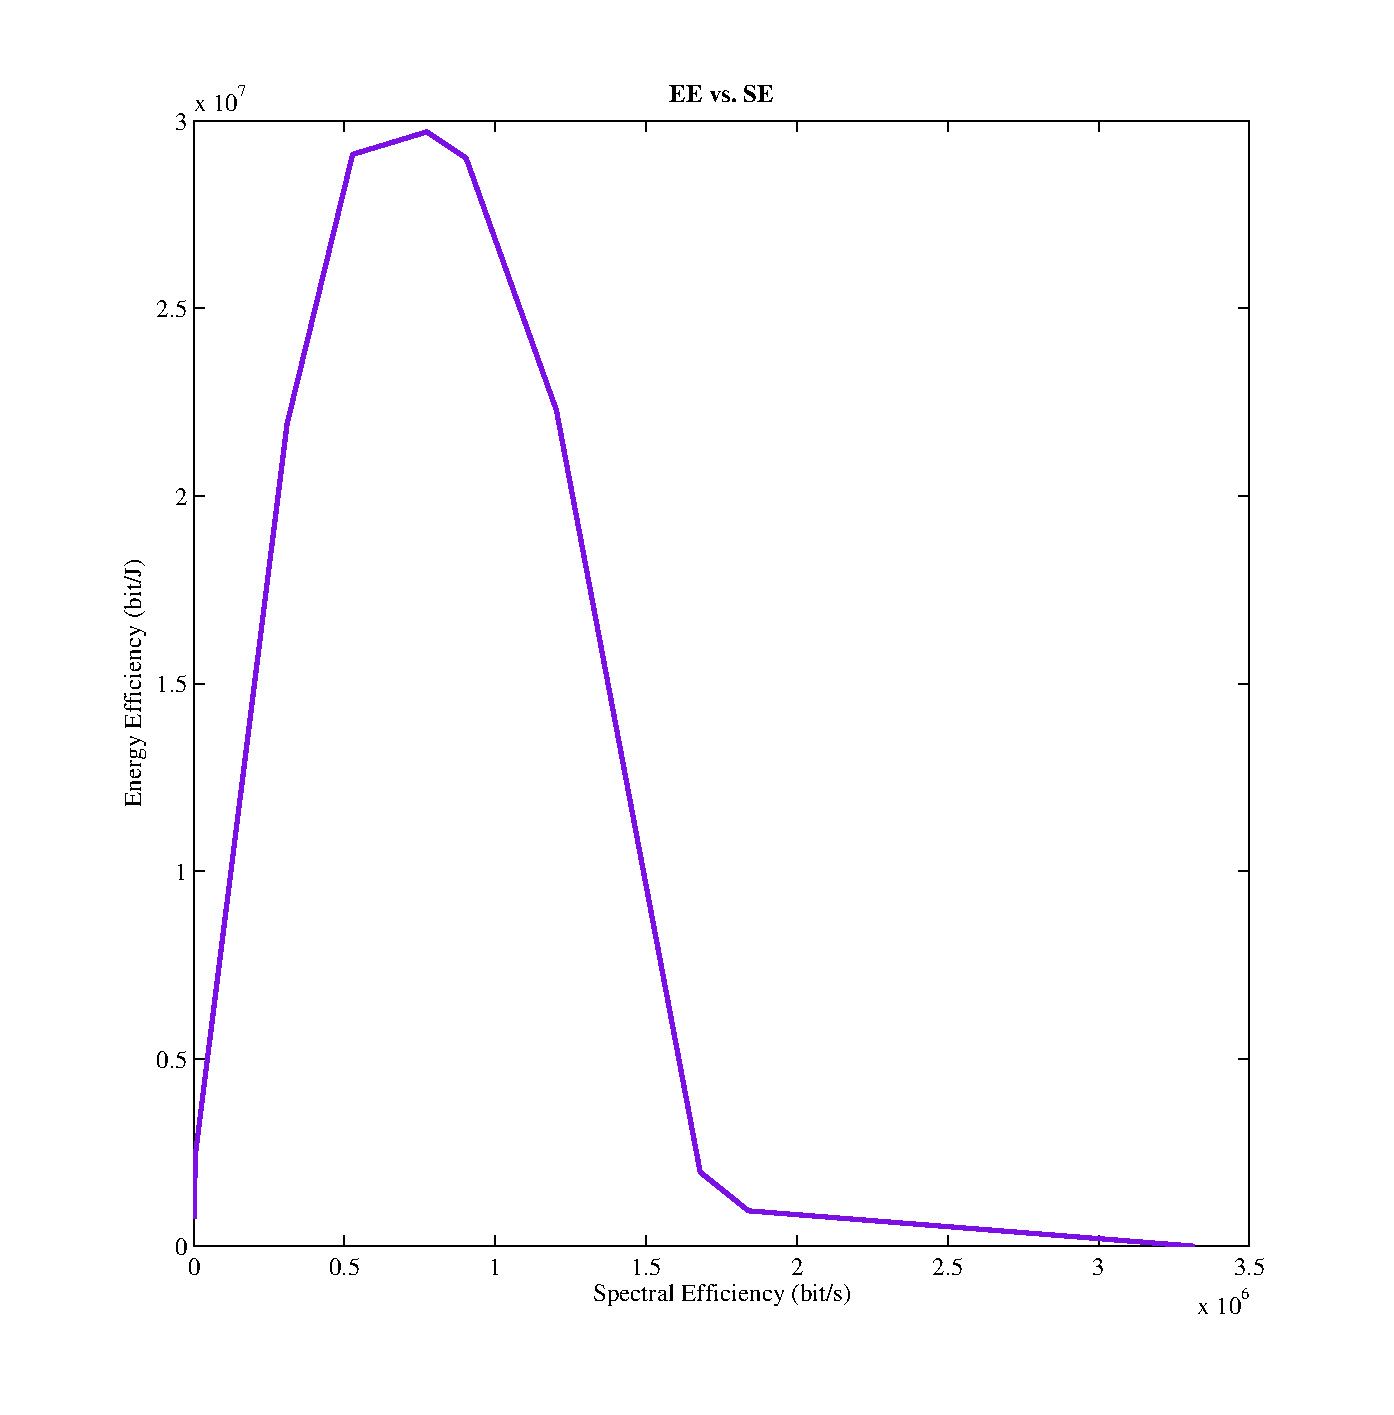
\includegraphics[width=\linewidth]{./fig3/spect}
%  \caption{  بازدهی انرژی بر حسب بازدهی طیف}
%  \label{fig:spect}
%\end{figure}
%در شکل \ref{fig:spect}، بازدهی انرژی بر حسب بازدهی طیف برای 2 خوشه که در هر خوشه 2 کاربر و 10 واحد رادیویی قرار دارد ($\sigma_q = 10^{-4}$)، رسم شده است. این نمودار با تغییر توان بیشینه ی هر واحد رادیویی رسم شده است. ابتدا با افزایش توان از مقدار 0 بازدهی انرژی بر حسب بازدهی طیف زیاد می شود و در نهایت با افزایش توان بازدهی انرژی بر حسب بازدهی طیف کاهش می یابد.  
\subsection{نتیجه گیری}
در این بخش، تخصیص توان بهینه در لینک فروسو برای مدل سیستم \lr{MIMO C-RAN} با فرض محدودیت بر روی ظرفیت \lr{fronthaul}، در نظر گرفته شده است. مدل سیستم شرح داده شده و مسئله ی تخصیص توان بهینه با روش الگوریتم بهینه و استفاده از تابع لاگرانژ حل شده است. شبیه سازی ها نشان می دهد که با افزایش تعداد واحدهای رادیویی عملکرد سیستم بهبود داده و افزایش تعداد کاربران ابتدا منجر به افزایش بازدهی انرژی می گردد و سپس به دلیل زیاد شدن تاثیر تداخل، \lr{EE} کاهش می یابد. همچنین با کاهش نویز کوانتیزاسیون عملکرد سیستم بهبود می یابد. علاوه بر این، با افزایش  بیشینه ظرفیت لینک \lr{fronthaul} ابتدا بازدهی انرژی زیاد شده سپس شیب افزایش بازدهی انرژی، کم می شود.
%%%%%%%%%%%%%%%%%%%%%%%%%%%%%%%%%%%%%%%%%%%%%%%%%
\section{لینک فراسو}
در این بخش، لینک فراسو برای سیستم \lr{MIMO C-RAN} در نظر گرفته شده است که  پیام در مسیر لینک فراسو از کاربر به واحدهای رادیویی منتقل می شود و پس از فشرده سازی توسط لینک \lr{fronthaul} به واحد کنترل منتقل می گردد. \newline
همانند لینک فروسو فرض بر این است که واحدهای رادیویی و کاربران خوشه بندی شده اند به طوری که هر خوشه  شامل تعدادی واحد رادیویی است که به کاربران موجود در آن خوشه، سرویس دهی می کنند.

 \begin{figure}
  \centering
    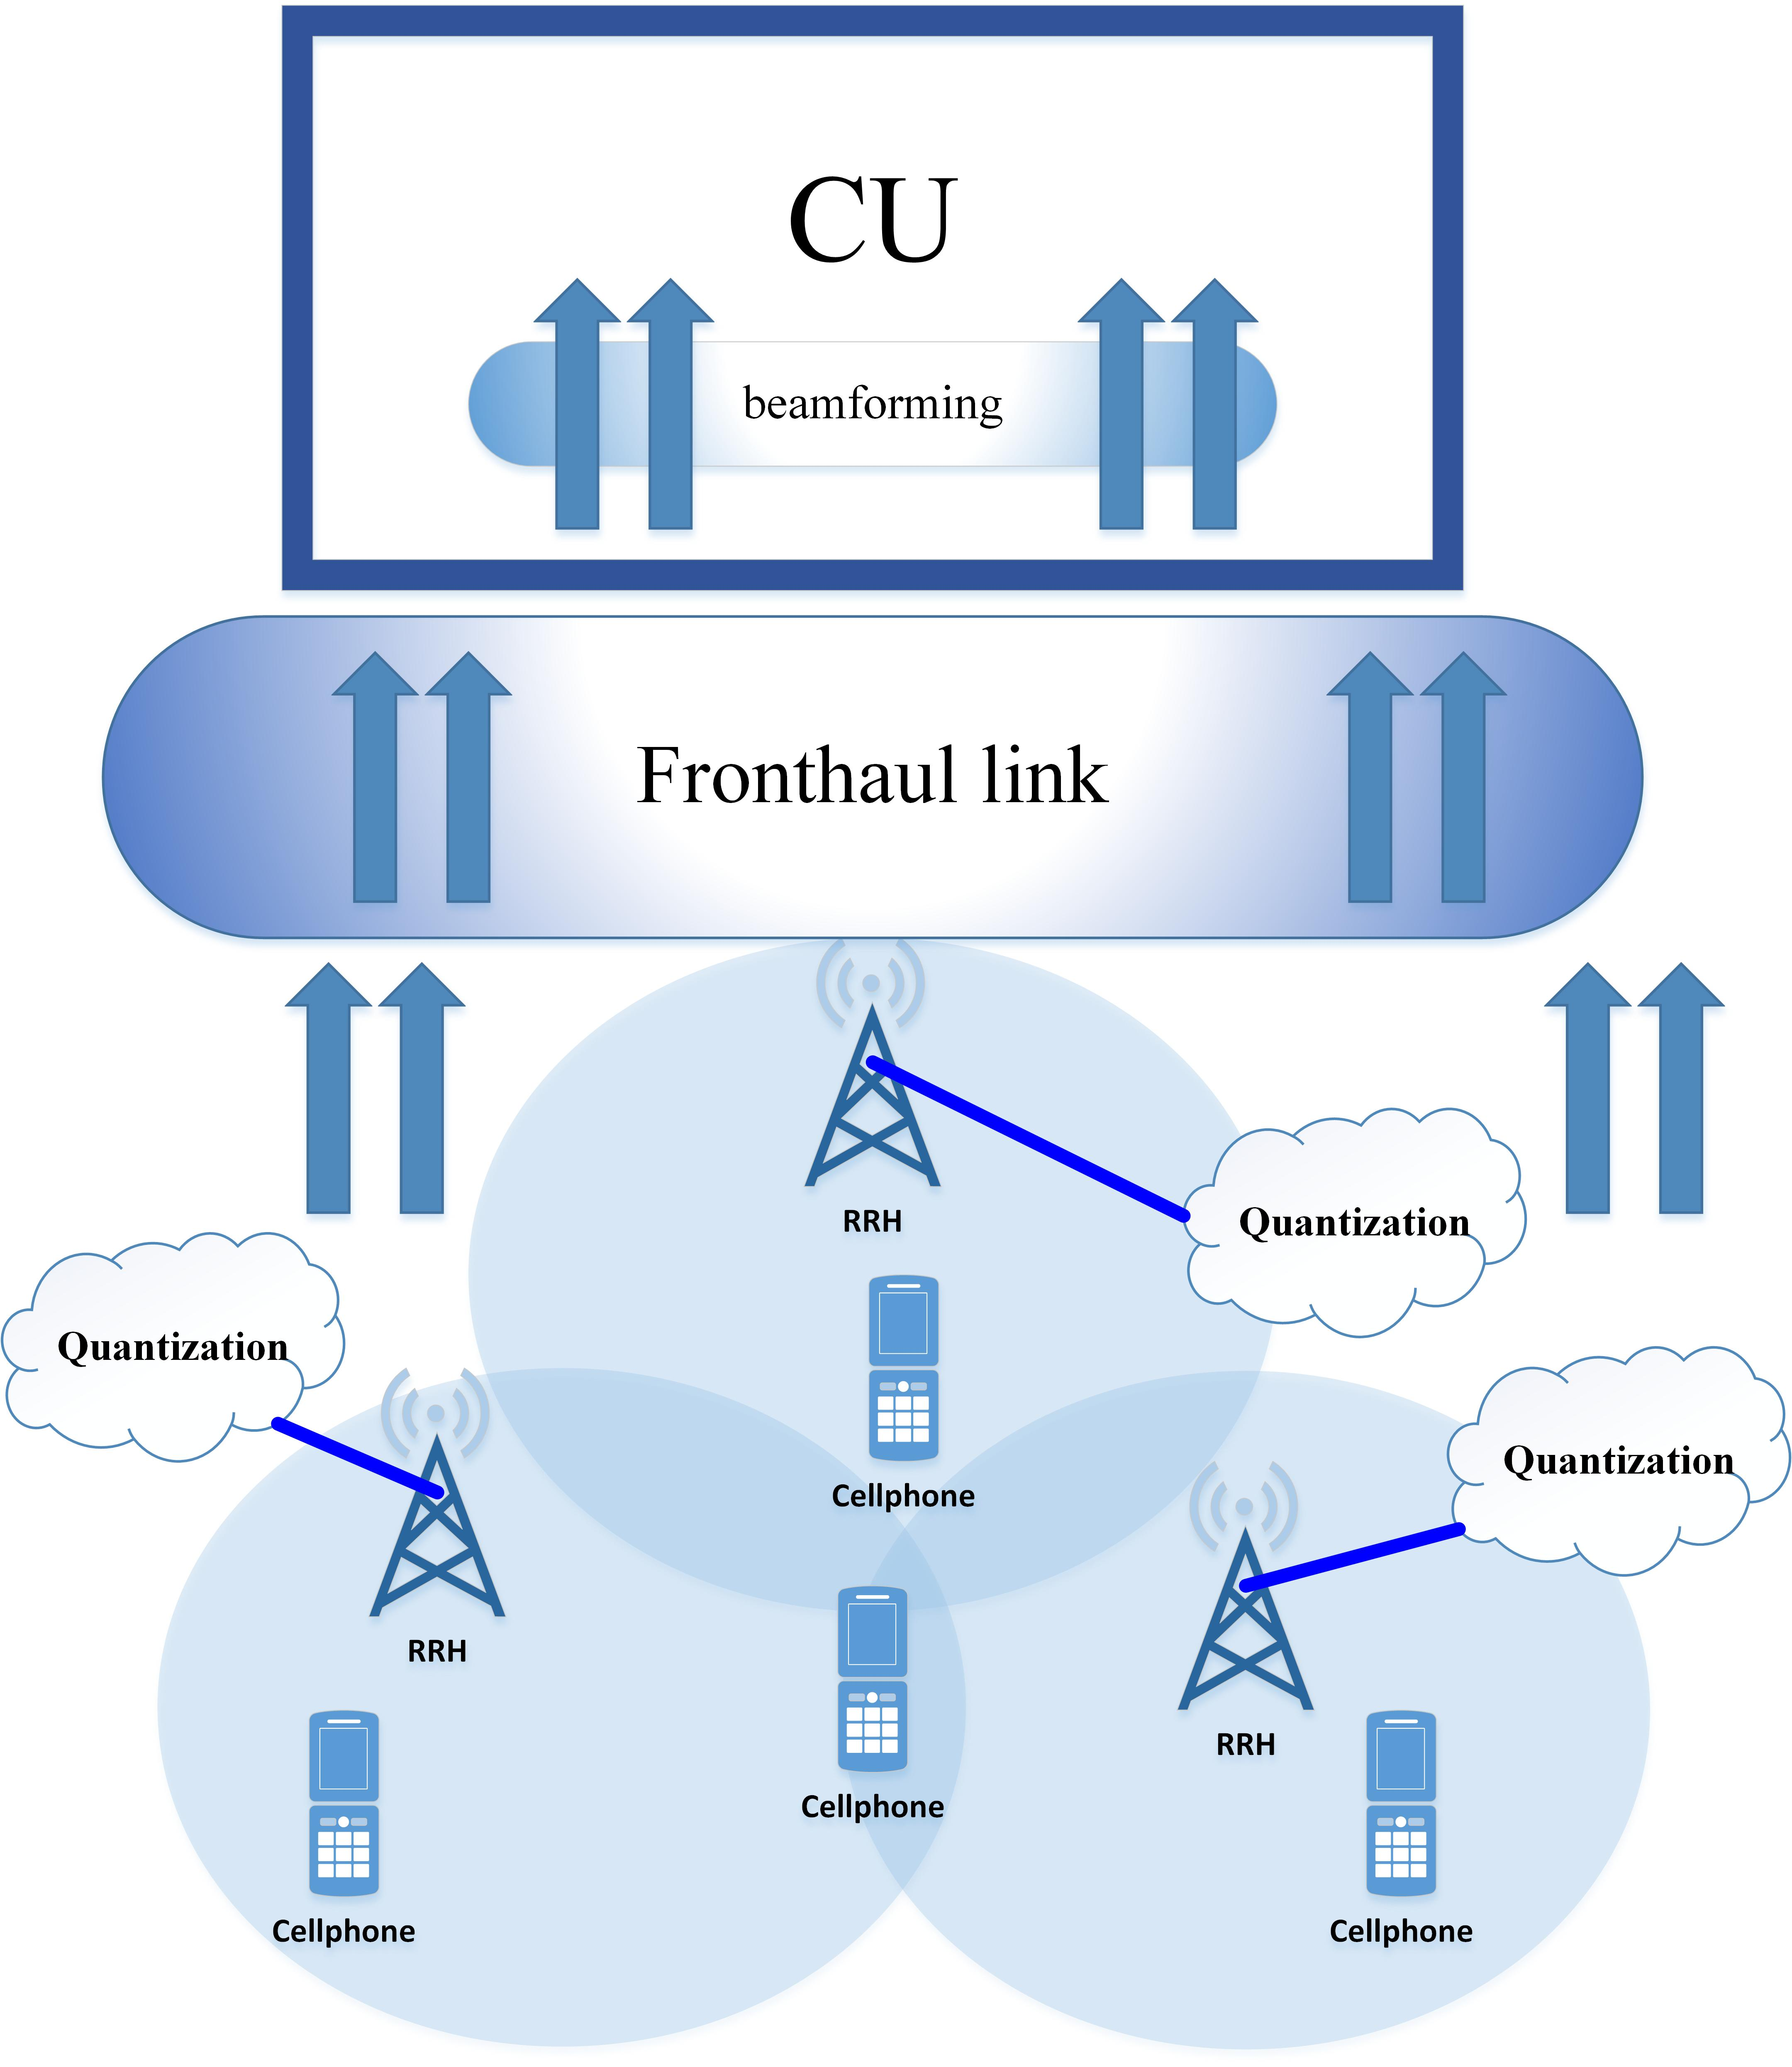
\includegraphics[scale = 0.45]{./fig/Drawing2}
  \caption{ساختار 
  \lr{C-RAN}
  در  لینک فراسو
  }
  \label{fig:cr2}
\end{figure}
همچنین در این مدل از روش پرتو دهی برای کاهش تداخل استفاده می کنیم که پرتو دهی در داخل واحد کنترل صورت می گیرد.
در ادامه، ابتدا سیستم  مدل و سپس نرخ قابل دسترسی بیان شده و مسئله ی تخصیص توان بررسی می گردد.
\subsection{مدل سیستم}
مدل سیستم برای لینک فراسو نیز همانند لینک فروسو می باشد که در ادامه شرح داده شده است\cite{ofdma,ulCompression}.
 سیستم \lr{MIMO C-RAN} شامل $R$ واحد رادیویی می باشد که $D$ کاربر تک آنتنه را سرویس می دهند.فرض بر این است که کاربران و واحد رادیوییها، به 
 $S$
خوشه تقسیم شده اند که $v$ امین خوشه،
 دارای $R_v$ واحد رادیویی است که ${D}_v$ کاربر را سرویس دهی می کنند.
 علاوه بر این، فرض بر این است که
$j$
امین واحد رادیویی، در $v$امین خوشه، توسط لینک فیبر نوری با ظرفیت محدود $c_{r_{(v,j)}}$ به واحد کنترل متصل می گردد.
\begin{equation}
\begin{split}
\mathcal{R}_v= \{  r_{(v,i)} | 1 \leq i \leq {R}_v , i\in Z^+\}, \\
\mathcal{C}_{\mathcal{R}_v}= \{C_{r_{(v,j)}}| 1 \leq j \leq {R}_v , j\in Z^+\}, \\
\mathcal{D}_v= \{  d_{(v,k)} | 1 \leq k \leq {D}_v , k\in Z^+\},  \\
\end{split}
\end{equation} 
که
 $\mathcal{R}_v$، $\mathcal{C}_{\mathcal{R}_v}$
 و
  $\mathcal{D}_v$
 به ترتیب نشان دهنده ی دسته واحد رادیوییها، دسته ی ظرفیت لینک \lr{Fronthaul} و دسته ی کاربران در $v$امین دسته ی خوشه می باشد.\newline
واحد رادیویی
ها تداخل پیام ها را از خوشه های دیگر نیز دریافت می کنند.\newline
 \subsection{آنالیز نرخ قابل دسترس}
در این قسمت، هدف بررسی نرخ قابل دسترسی سیستم می باشد.
\begin{theorem}\label{t1}
 نرخ قابل دسترسی برای کاربر $d_{(s,k)}$ به صورت زیر می باشد:
\begin{equation}\label{e1}
\mathfrak{R}_{d_{(s,k)}} = B \log_2(1+\gamma_{d_{(s,k)}}),
\end{equation}
که $B$ پهنای باند کانال و $\gamma_{d_{(s,k)}}$ همان \lr{SINR} دریافتی $k$امین کاربر در $s$امین دسته ی خوشه است که به صورت زیر بیان می گردد.  
\begin{equation}\label{5}
\gamma_{d_{(s,k)}}= \frac{p_{d_{(s,k)}} |{\boldsymbol{w}^H}_{\mathcal{R}_{s},d_{(s,k)}}^آ\boldsymbol{h}_{\mathcal{R}_s, d_{(s,k)}}|^2}{I_{d_{(s,k)}}+B\nu}.
\end{equation}
در فرمول \eqref{5}، 
$I_{d_{(s,k)}}$
نشان دهنده ی توان سیگنال تداخلی است.$B\nu$
نشان دهنده ی توان نویز است و
$\boldsymbol{h}_{\mathcal{R}_s, d_{(s,k)}}$ 
 نشان دهنده ی بردار کانال بین $k$امین کاربر و واحدهای رادیویی
 $s$
 امین دسته ی خوشه می باشد. همچنین 
 $\boldsymbol{w}_{\mathcal{R}_{s},d_{(s,k)}}$
 نشان دهنده ی بردار پرتو دهی استفاده شده در $s$امین دسته ی خوشه ها برروی واحدهای رادیویی برای بدست آوردن پیام $k$امین کاربر می باشد. 
 $p_{d_{(s,k)}}$
 توان ارسالی$k$امین کاربر در $s$امین دسته ی خوشه می باشد.
\end{theorem}
\begin{proof}
در این قسمت می خواهیم $\gamma$ را بدست آوریم

فرض کنید $\boldsymbol{y}_{\mathcal{R}_s}$ یک بردار
 $R_s \times 1$
باشد که نشان دهنده ی سیگنال دریافتی توسط دسته ای از واحدهای رادیویی در $s$
امین خوشه باشد که به صورت زیر بدست می آید.
\begin{equation} \label{1}
\boldsymbol{y}_{\mathcal{R}_s} = \sum_{v=1}^S \boldsymbol{H}_{\mathcal{R}_v,\mathcal{D}_s}{\boldsymbol{x}}_{\mathcal{D}_v}+ \boldsymbol{z}_{\mathcal{D}_s},
\end{equation}
که   ${\boldsymbol{x}}_{ \mathcal{D}_v} = [{x}_{ d_{(v,1)}},...,{ x}_{ d_{(v,\mathcal{D}_v)}}]^T \in \mathbb{C}^{{D}_v } $ 
بردار سمبل ارسالی خوشه ی  $v$ ام می باشد.\newline
 $\boldsymbol{z_{\mathcal{D}_s}} \backsim \mathcal{N}(0,N_0\boldsymbol{I}_{{D}_s})$ 
 نویز گوسی سفید اضافه شونده می باشد که دارای توان $N_0$
 و \newline
 $\boldsymbol{H}_{\mathcal{R}_v,\mathcal{D}_s}  \in \mathbb{C}^{{R}_v\times {D}_s}$ 
 نشان دهنده ی ماتریس کانال بین  کاربران $\mathcal{D}_s$ در دسته ی
 $s$
   ام و واحدهای رادیویی   $\mathcal{R}_v$ در دسته ی   $v$ ام می باشد.\newline
همچنین مدل کانال همانند لینک فروسو با توجه به فرمول \eqref{channel}، بدست می آید.
 حال می خواهیم پیام دریافتی توسط واحد رادیویی  $n$ ام در دسته ی $s$ ام را بدست آوریم:
 
\begin{equation} \label{100}
y_{r_{(s,n)}} = \sum_{k=1}^{D_s} h_{r_{(s,n)},d_{(s,k)}} \sqrt{p_{d_{(s,k)}}}  x_{d_{(s,k)}}
+\sum_{t=1,t\neq s}^{S} \sum_{j=1}^{D_t} h_{r_{(s,n)},d_{(t,j)}} \sqrt{p_{d_{(t,j)}}} x_{d_{(t,j)}}
 +z_{r_{(s,n)}}
\end{equation}
پیام دریافتی توسط واحد رادیویی، بعد از فشرده سازی به صورت زیر می شود
\begin{equation}
\hat{y}_{r_{(s,n)}} = y_{r_{(s,n)}} + q_{r_{(s,n)}} 
\end{equation}
پیام هر کاربر در واحد کنترل با اعمال پرتو دهی \LTRfootnote{beamforming} به صورتی که در ادامه بیان شده، بدست می آید

\begin{equation}
\begin{split}
\hat{x}_{d_{(s,k)}} = & {\boldsymbol{w}^H}_{\mathcal{R}_s, d_{(s,k)}} \boldsymbol{h}_{\mathcal{R}_s, d_{(s,k)}} \sqrt{p_{d_{(s,k)}}}  x_{d_{(s,k)}} \\
+ & \sum_{i=1,i\neq k}^{D_s}  {\boldsymbol{w}^H}_{\mathcal{R}_s, d_{(s,k)}} \boldsymbol{h}_{\mathcal{R}_s, d_{(s,i)}} \sqrt{p_{d_{(s,i)}}}  x_{d_{(s,i)}} \\
+&  \sum_{t=1,t\neq s}^{S} \sum_{j=1}^{D_t} {\boldsymbol{w}^H}_{\mathcal{R}_s, d_{(s,k)}} \boldsymbol{h}_{\mathcal{R}_s, d_{(t,j)}} \sqrt{p_{d_{(t,j)}}}  x_{d_{(t,j)}} \\
+& {\boldsymbol{w}^H}_{\mathcal{R}_s, d_{(s,k)}}  ({\boldsymbol{q}}_{\mathcal{R}_s} + {\boldsymbol{z}}_{\mathcal{R}_s})
\end{split}
\end{equation}
حال برای بدست آوردن  \lr{SINR}، توان سیگنال بر روی توان تداخل و نویز را بدست می آوریم:
\begin{equation}
\gamma = \frac{p_{d_{(s,k)}}|{\boldsymbol{w}^H}_{\mathcal{R}_s, d_{(s,k)}} \boldsymbol{h}_{\mathcal{R}_s, d_{(s,k)}}|^2}{
  I_{d_{(s,k)}}
+ B \times \nu_{d_{(s,k)}}
}
\end{equation}
که داریم :
\begin{equation}
\begin{split}
\nu_{d_{(s,k)}}&  = {\boldsymbol{w}^H}_{\mathcal{R}_s, d_{(s,k)}}  (diag({\sigma_n^2}_{r_{(s,1)}}...{\sigma_n^2}_{r_{(s,R_s)}})+diag({\sigma_q^2}_{r_{(s,1)}}...{\sigma_q^2}_{r_{(s,R_s)}})) {\boldsymbol{w}}_{\mathcal{R}_s, d_{(s,k)}}\\
I_{d_{(s,k)}}& = \sum_{i=1,i\neq k}^{D_s}  |{\boldsymbol{w}^H}_{\mathcal{R}_s, d_{(s,k)}} \boldsymbol{h}_{\mathcal{R}_s, d_{(s,i)}}|^2 p_{d_{(s,i)}} +\sum_{t=1,t\neq s}^{S} \sum_{j=1}^{D_t} |{\boldsymbol{w}^H}_{\mathcal{R}_s, d_{(s,k)}} \boldsymbol{h}_{\mathcal{R}_s, d_{(t,j)}}|^2 p_{d_{(t,j)}} 
\end{split}
\end{equation}
 در اینجا  $\sigma_n^2$ واریانس نویز می باشد که  برای سادگی برای همه ی واحدهای رادیویی ثابت فرض شده و  دارای مقدار $N_0$ 
است و $\sigma_q^2$ واریانس نویز فشرده سازی می باشد.
علاوه بر این با استفاده از پرتودهی \lr{MMSE}، ماتریس پرتودهی به صورت زیر است 
\begin{equation}
\boldsymbol{W}_{\mathcal{R}_s,\mathcal{D}_s} = \hat{\boldsymbol{H}}_{\mathcal{R}_s,\mathcal{D}_s}(\hat{\boldsymbol{H}}_{\mathcal{R}_s,\mathcal{D}_s}^H \hat{\boldsymbol{H}}_{\mathcal{R}_s,\mathcal{D}_s}+ \alpha \boldsymbol{I}_{{D}_s})^{-1},
\end{equation} 
همچنین  $\alpha$، فاکتور رگولاریزاسیون است در صورتی که $\alpha$ صفر یاشد، ماتریس پرتو دهی \lr{ZF} خواهیم داشت.
\end{proof}
\subsection{بهینه سازی تخصیص توان}
در این قسمت می خواهیم توان را طوری اختصاص دهیم تا بازدهی انرژی به بیشینه مقدار خود برسد.
می دانیم نرخ قابل دسترس بر روی لینک \lr{fronthaul}، بین $n$ امین واحد رادیویی در $s$ امین خوشه  و  واحد کنترل به صورت زیر بدست می آید 
\begin{equation}
C_{r_{(s,n)}} = \log{\frac{1+( \sum_{k=1}^{D_s}|h_{r_{(s,n)},d_{(s,k)}}|^2{p_{d_{(s,k)}}} + \sum_{t=1,t\neq s}^{S}\sum_{l=1}^{D_t}|h_{r_{(s,n)},d_{(t,l)}}|^2{p_{d_{(t,l)}}}+ B N_0) }{ \sigma_{q_{(s,n)}}^2})},
\end{equation}
\subsubsection{شرح مسئله}
 همانطور که گفته شد نسبت مجموع نرخ ها در سیستم به کل توان ارسالی کاربرها نشان دهنده ی بازدهی انرژی است که با $\eta$ نمایش داده می شود و می توان اینگونه بیان کرد
\begin{equation}\label{eta1}
\eta(\boldsymbol{P}) := \frac{\sum\limits_{s=1}^{S} \sum\limits_{k=1}^{{D}_s}\mathfrak{R}_{d_{(s,k)}} }{\sum\limits_{s=1}^{S} \sum\limits_{k=1}^{{K}_s}{p}_{d_{(s,k)}}} = \frac{R_{total}(\boldsymbol{P})}{P_{UE}(\boldsymbol{P})},
\end{equation}
که در اینجا  $ \boldsymbol{P} = \{ \boldsymbol{P}_{\mathcal{D}_s}|  1 \leq s \leq S, s \in \mathbb{Z}^{+} \}$ ماتریس تخصیص توان است. در این بخش، بیشینه سازی بازدهی انرژی با شروط زیر مورد بررسی قرار می گیرد 
\begin{equation}\label{p11}
\begin{aligned}
\max\limits_{\boldsymbol{P}}   \quad &   \eta(\boldsymbol{P})\\
\text{\lr{subject to}} \quad  &  0 \leq {p}_{d_{(s,k)}} \leq P_{max} && \qquad \forall s, \forall k,   \\
&\mathfrak{R}_{d_{(s,k)}} \geq  \mathfrak{R}_{d_{(s,k)}}^{th} && \qquad \forall s, \forall k, \\ 
&C_{r_{(s,i)}} \leq C_{r_{(s,i)}}^{th}  &&\qquad \forall s, \forall i, \\
\end{aligned}			
\end{equation}
همانند لینک فروسو، بدلیل محدب نبودن مسئله از روش الگوریتم تکرار شونده استفاده می کنیم.
\subsection{روش مورد استفاده}
در این قسمت، به جای ماکسیمم کردن \eqref{eta1}، همانند لینک فروسو، از قضیه ی \eqref{t2} استفاده می نماییم.
 همچنین کران بالایی برای تداخل بدست می آید که در ادامه بیان می شود.
\begin{equation} \label{id}
\tilde{I}_{d_{(s,k)}} = \sum_{v=1}^{S}  |{\boldsymbol{w}^H}_{\mathcal{R}_s, d_{(s,k)}} \boldsymbol{h}_{\mathcal{R}_v, d_{(s,i)}}|^2 P_{max} 
\end{equation}
در نتیجه با توجه به رابطه ی  \eqref{id}، می توان $\gamma$ را به این صورت تخمین زد:
\begin{equation}
\tilde{\gamma}_{d_{(s,k)}}= \frac{p_{d_{(s,k)}} |{\boldsymbol{w}^H}_{\mathcal{R}_{s},d_{(s,k)}}^آ\boldsymbol{h}_{\mathcal{R}_s, d_{(s,k)}}|^2}{\tilde{I}_{d_{(s,k)}}+B\nu}.
\end{equation}
ابتدا تابع لاگرانژ را تشکیل می دهیم تا بتوان با استفاده از آن، از الگوریتم تکرار شونده ی \eqref{alg}، استفاده کرد. 
\begin{equation}
\begin{split}
\mathcal{L}(\boldsymbol{P}; \boldsymbol{\lambda}, \boldsymbol{\mu}, \boldsymbol{ \kappa}) & = \sum\limits_{s=1}^{S} \sum\limits_{k=1}^{\mathcal{D}_s}\mathfrak{\tilde{R}}_{d_{(s,k)}} 
- \eta \sum\limits_{s=1}^{S} \sum\limits_{k=1}^{\mathcal{K}_s}{p}_{d_{(s,k)}}\\
&+\sum\limits_{s=1}^{S} \sum\limits_{k=1}^{\mathcal{D}_s} \lambda_{d_{(s,k)}} (\mathfrak{\tilde{R}}_{d_{(s,k)}}-\mathfrak{R}_{d_{(s,k)}}^{th})\\
&- \sum\limits_{s=1}^{S} \sum\limits_{k=1}^{\mathcal{K}_s} \mu_{d_{(s,k)}} ({p}_{d_{(s,k)}}-P_{max})\\
&- \sum\limits_{s=1}^{S} \sum\limits_{i=1}^{\mathcal{R}_s} \kappa_{r_{(s,i)}} (C_{r_{(s,i)}}-C_{r_{(s,i)}}^{th}).\\
\end{split}
\end{equation}
که در اینجا، $\boldsymbol{\lambda}, \boldsymbol{\mu}, \boldsymbol{\kappa} \geq 0$
بردارهای ضرایب لاگرانژ می باشد .\newline
با استفاده از این معادله و مشتقگیری از آن، توان بهینه به صورت زیر بدست می آید
\begin{equation}
p_{d_{(s,k)}}^* \approx [\frac{ B(1+\lambda_{d_{(s,k)}} )-(\sum_{n=1}^{\mathcal{R}_s}\kappa_{r_{(s,i)}})}{\ln2 \times (\eta + \mu_{d_{(s,k)}})}]^+;
\end{equation} 

  در آخر، برای بدست آوردن توان بهینه، الگوریتم \eqref{alg1} مورد استفاده قرار می گیرد \cite{hcranEE}
 \begin{latin}
\begin{algorithm}
\caption{Energy-Efficient Power Allocation}\label{alg1}
\begin{algorithmic}

\State Set the maximum number of iterations $I_{max}$, convergence condition $\epsilon_{\eta}$  and the initial value $\eta^{(1)} = 0$
\State Set the iteration index $i = 1$ and begin the iteration (Outer
Loop).
\For {$ 1\leq i \leq  Imax$}
\State Solve the resource allocation problem with $\eta^{(i)}$ (Inner Loop);
\State Obtain $P^{(i)}, R_{total}^{(i)}, P_{UE}^{(i)}$
\If {$ R_{total}(\boldsymbol{P}^{(i)}) - \eta^{(i)} P_{UE}(\boldsymbol{P}^{(i)}) < \epsilon_{\eta} $} 
\State Set $\boldsymbol{P}^*= \boldsymbol{P}^{(i)} $   and  $ \eta^{*} =\eta^{(i)} $;
\State break;
\Else
\State Set $\eta^{(i)}= \frac{R_{total}(\boldsymbol{P}^{(i))}}{P_{UE}(\boldsymbol{P}^{(i))}}$ and $i= i+1$;
\EndIf 
\State \textbf{end if}
\EndFor 
\State \textbf{end for}

\end{algorithmic}
\end{algorithm}
\end{latin}
\subsection{نتایج عددی}
در این بخش، نتایج عددی الگوریتم مورد استفاده را برای سیستم \lr{MIMO C-RAN} با پارامترهای بیان شده در جدول \ref{tab:title3} و استفاده از پرتو دهی \lr{ZF} بیان می شود.
\begin{latin} 
 \begin{table}[H]
 \caption {\rl{پارامترهای شبیه سازی}} \label{tab:title3} 
 \begin{center}
  \begin{tabular}{||c c ||} 
  \hline
  Parameter & Value \\ [0.5ex] 
  \hline\hline
  Number of cluster S & 3 \\ 
  \hline
  Noise power density & -174dBm/Hz\\
  \hline
  Bandwidth & 120KHz \\
  \hline
 Maxmimun transmit Power & 10dBm \\
  \hline
  Circuit Power of whole RRHs & 10dBm \\
  \hline
  Variance of quantization noise & $10^{-2}$ \\
  \hline
   Maxmimun fronthaul link's rate & 20bits/sec/Hz \\
  \hline
  Minimum data rate &  1bits/sec/Hz \\ [1ex] 
  \hline
 \end{tabular}
 \end{center}
 \end{table}
 \end{latin}
  \begin{figure}[H]
  \centering
    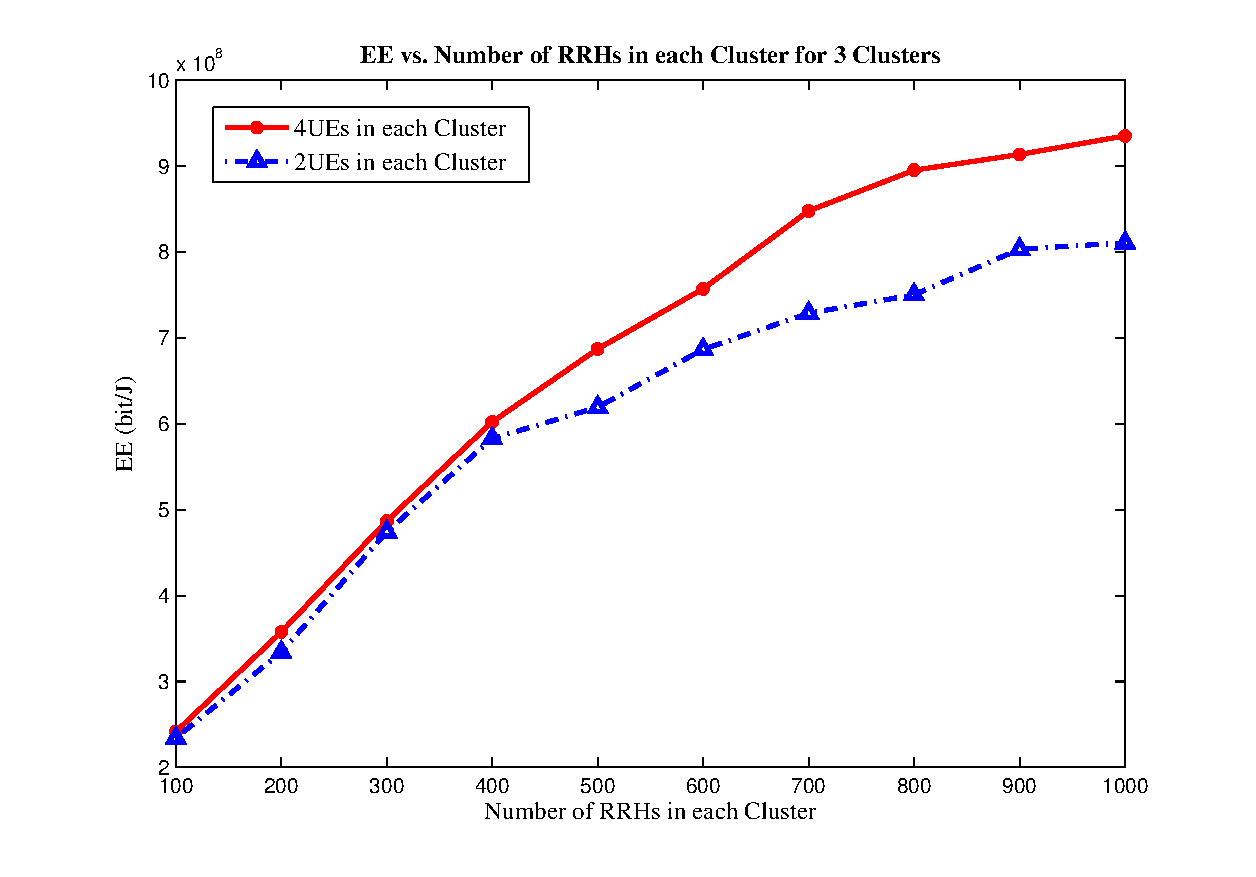
\includegraphics[width=\linewidth, height=12cm]{./fig3/rrhul}
  \caption{
  بازدهی انرژی با توجه به تغییرات تعداد واحدهای رادیویی  در هر خوشه برای توان بهینه  برای 
   دو کاربر مختلف
   و پارامترهای جدول \ref{tab:title3}}
  \label{fig:rrhul}
\end{figure}
 در شکل \ref{fig:rrhul}، بازدهی انرژی سیستم \lr{MIMO C-RAN} بر اساس تعداد واحدهای رادیویی در هر خوشه برای الگوریتم مورد استفاده و برای دو تعداد کاربر متفاوت، رسم شده است. 
 همانطور که  شکل  نشان می دهد، با افزایش تعداد واحدهای رادیوی، بازدهی انرژی افزایش می یابد و از یک مقدار به بعد شیب افزایش بازدهی انرژی کمتر شده است. زیرا با افزایش تعداد واحدهای رادیویی، مجموع توان کل افزایش یافته و در نتیجه نرخ انتقال داده نیز بیشتر می گردد.

 \begin{figure}[H]
  \centering
    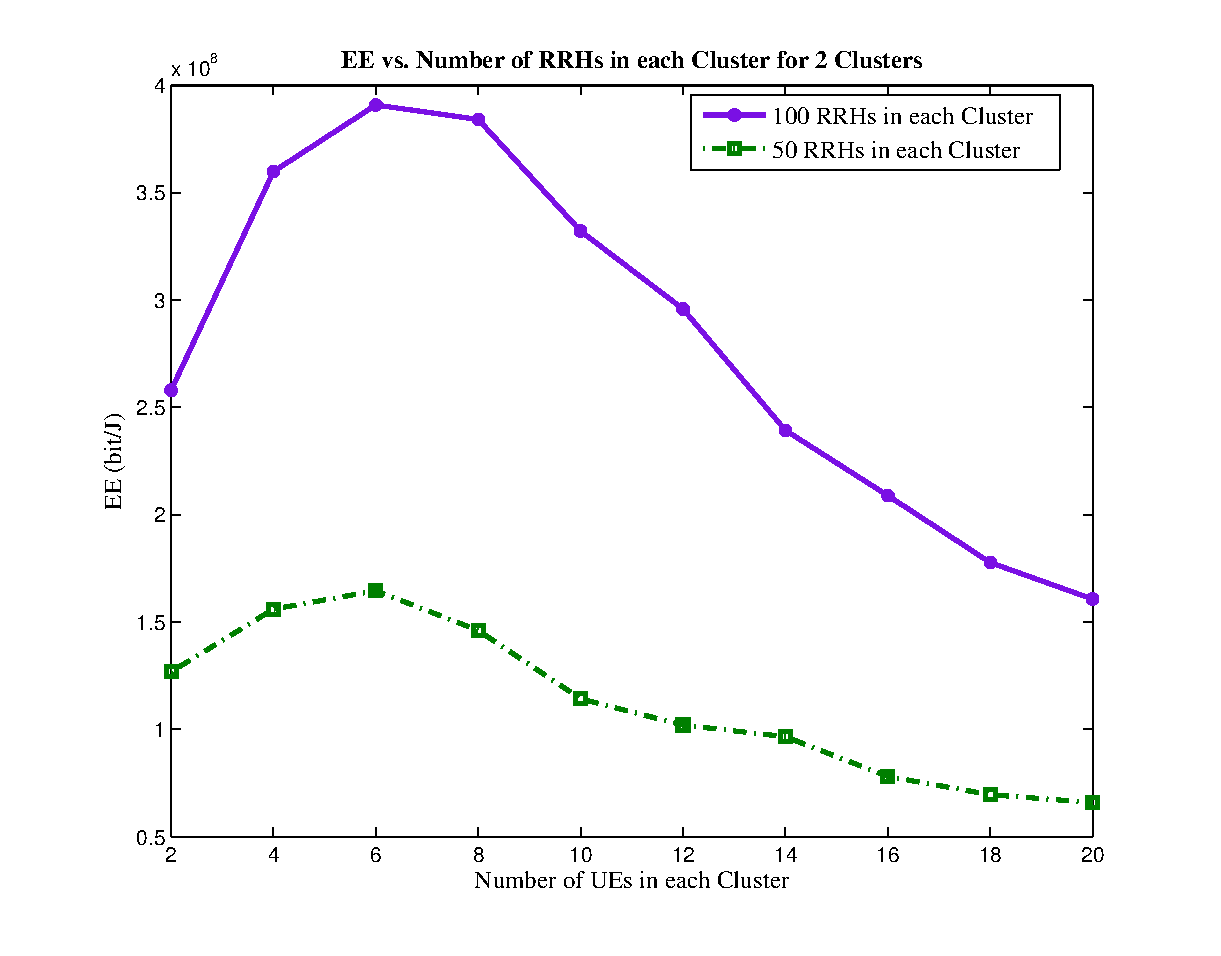
\includegraphics[width=\linewidth]{./fig3/ueul}
  \caption{  بازدهی انرژی با توجه به تغییرات تعداد کاربران در هر خوشه برای توان بهینه برای 
   دو واحد رادیویی مختلف
   و پارامترهای جدول \ref{tab:title3} و $S=2$}
  \label{fig:ueul}
\end{figure}


در شکل \ref{fig:ueul}، بازدهی انرژی بر اساس تعداد کاربران در هر خوشه برای الگوریتم مورد استفاده و برای دو تعداد واحد رادیویی متفاوت، رسم شده است. همانطور که  دیده می شود با افزایش تعداد کاربران، ابتدا شیب نمودار زیاد می شود و بازدهی انرژی افزایش می یابد سپس به دلیل افزایش تاثیر تداخل بین کاربران بازدهی انرژی کاهش می یابد. 

\begin{figure}[H]
  \centering
    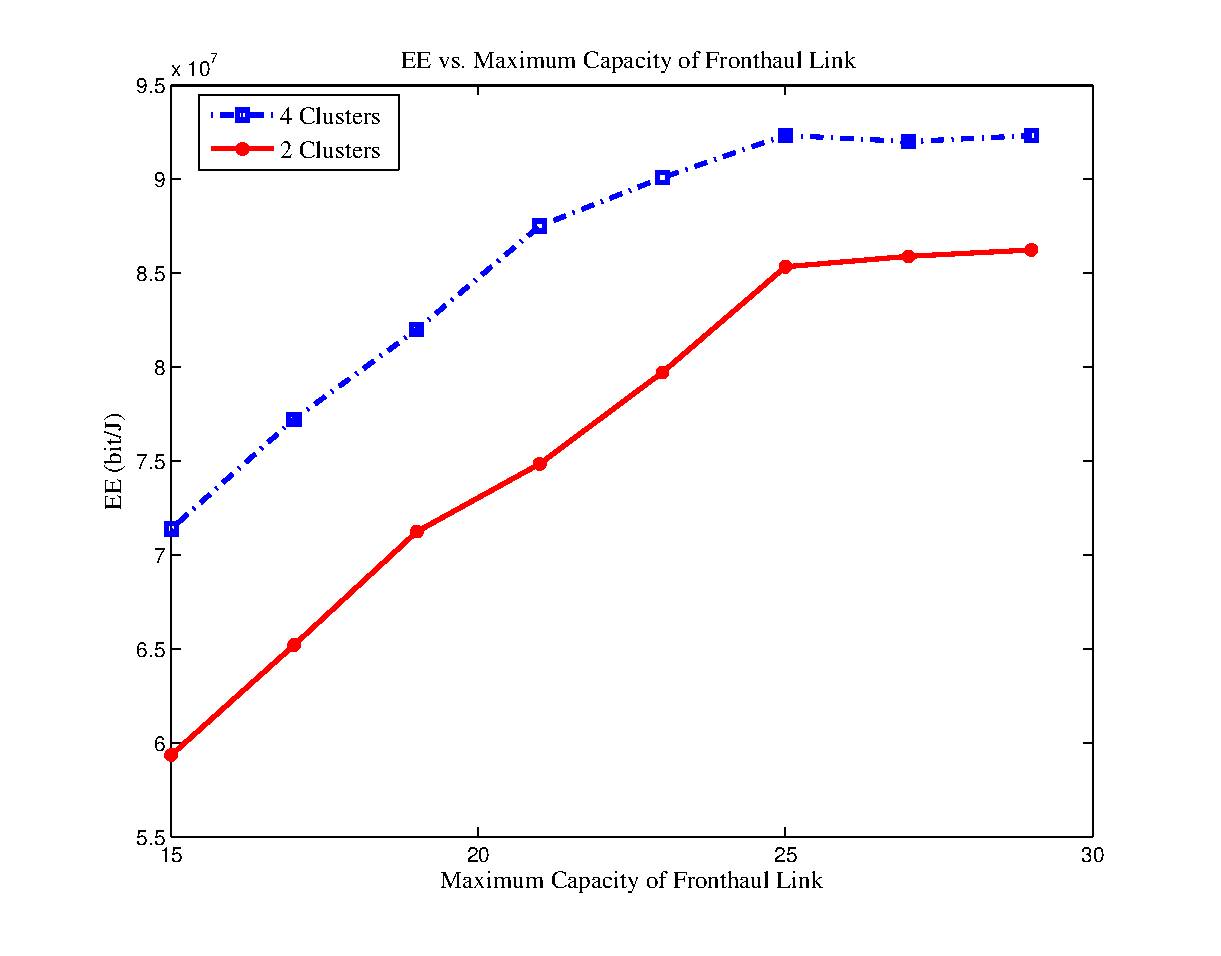
\includegraphics[width=\linewidth]{./fig3/cap}
  \caption{  بازدهی انرژی با توجه به تغییرات $C^{th}$، در در حالت $S =2 ,4 $, $\text{\lr{Number of RRHs per Cluster}} = 30$, $\text{\lr{Number of UE per Cluster}} =2$ }
  \label{fig:cap}
\end{figure}

در شکل \ref{fig:cap}، بازدهی انرژی بر اساس محدودیت ظرفیت لینک \lr{fronthaul}، برای دو تعداد متفاوت  2 و 4 خوشه و در هر خوشه 2 کاربر و 30 واحد رادیویی رسم شده است. با توجه به شکل، ابتدا با بازدهی انرژی، افزایش یافته،
سپس بدلیل اینکه نرخ قابل دسترس توسط تعداد کاربران و واحدهای رادیویی محدود می گردد، به نظر می آید افزایش محدودیت این ظرفیت تاثیر چندانی در بازدهی انرژی ندارد.  
\subsection{نتیجه گیری}
در این بخش، تخصیص توان بهینه در لینک فراسو برای مدل سیستم \lr{MIMO C-RAN} با فرض محدودیت بر روی ظرفیت \lr{fronthaul} و وجود چندین خوشه، در نظر گرفته شده است. مدل سیستم  شرح داده شده و مسئله ی تخصیص توان بهینه با روش الگوریتم بهینه و استفاده از تابع لاگرانژ حل شده است. شبیه سازی ها نشان می دهد همانند لینک فروسو با افزایش تعداد واحدهای رادیویی عملکرد سیستم بهبود داده و افزایش تعداد کاربران منجر به افزایش بازدهی انرژی می گردد ولی در نهایت به دلیل تداخل بازدهی انرژی کاهش می یابد. همچنین، با افزایش  بیشینه ظرفیت لینک \lr{fronthaul} ابتدا بازدهی انرژی زیاد شده سپس شیب افزایش بازدهی انرژی، کم می شود.
%%%%%%%%%%%%%%%%%%%%%%%%%%%%%%%%%%%%%%%%%%%%%%		% فصل سوم: روش تحقیق
\chapter{تخصیص منابع در حالت تقسیم زمانی دینامیکی در شبکه دسترسی رادیویی}
\section{مقدمه}
در این فصل هدف بدست آوردن مدل سیستم در حالت تقسیم زمانی یا \lr{TDD} \LTRfootnote{Time Division Duplexing} دینامیکی می باشد که بدین منظور تخصیص توان برای هر دو لینک فراسو و فروسو به طور همزمان بدست می آید.
در تقسیم زمانی دینامیکی، منابع به صورت دینامیکی بین هر دو لینک فراسو و فروسو  تخصیص داده می شود. در سیستم های سنتی  ایستگاه پایه و سیستم سنتی ایستگاه پایه و واحد رادیویی که در فصل اول بیان شد، تداخل بین لینک فراسو و فروسو منجر به کاهش شدید در بازدهی انرژی می گردد در حالی که در سیستم \lr{C-RAN} این تداخل  به دلیل وجود \lr{BBU Pool} و واحد های رادیویی \lr{RRH} و نوع پردازش هایی که در آنها صورت می گیرد، تاثیر چندانی در بازدهی انرژی نمی گذارد \cite{TDD,dynamic}.


حال در ادامه، مدل سیستمی با ساختار \lr{C-RAN}  بیان می نماییم که دارای چندین خوشه است که تعدادی از این خوشه  ها در لینک فراسو و تعدادی دیگر در لینک فروسو عمل می کنند. همچنین تمام واحدهای رادیویی در این خوشه ها به واحد کنترل ابری \lr{BBU Pool} از طریق لینک \lr{fronthaul} با ظرفیت محدود، متصلند. سیگنالهای خوشه های لینک فراسو و فروسو نیز بر یکدیگر تداخل اعمال می کنند.
\section{مدل سیستم}
در این بخش مدل سیستمی برای حالت تقسیم زمانی دینامیکی  براساس معماری \lr{C-RAN} در لینک فراسو و فروسو همانند فصل 3 بیان می شود. فرض بر این است که این سیستم شامل $S$ خوشه می باشد که $S_1$ خوشه در لینک فروسو و $S_2$
 خوشه در لینک فراسو عمل می کنند که :
 $S_1 + S_2 = S$
 است.
 همچنین هر خوشه ی $v$ دارای  $R_v$  واحد رادیویی و $D_v$ کاربر می باشد.  
 علاوه براین، فرض بر این است که
$j$
امین واحد رادیویی، در $v$امین خوشه، توسط لینک فیبر نوری با ظرفیت محدود $C_{r_{(v,j)}}$ به واحد کنترل متصل می گردد. در نتیجه داریم:
\begin{equation}
\begin{split}
\mathcal{R}_v= \{  r_{(v,i)} | 1 \leq i \leq {R}_v , i\in Z^+\}, \\
\mathcal{C}_{\mathcal{R}_v}= \{C_{r_{(v,j)}}| 1 \leq j \leq {R}_v , j\in Z^+\}, \\
\mathcal{D}_v= \{  d_{(v,k)} | 1 \leq k \leq {D}_v , k\in Z^+\},  \\
\end{split}
\end{equation} 
که
 $\mathcal{R}_v$، $\mathcal{C}_{\mathcal{R}_v}$
 و
  $\mathcal{D}_v$
 به ترتیب نشان دهنده ی دسته واحدهای رادیویی، دسته ی ظرفیت لینک \lr{Fronthaul} و دسته ی کاربران در $v$امین دسته ی خوشه می باشد.\newline
واحدهای رادیویی
 تداخل پیام ها را از خوشه های دیگر لینک فراسو و فروسو دریافت می کنند.
\newline
 \subsection{آنالیز نرخ قابل دسترس در خوشه های فروسو}
در این قسمت، هدف بررسی نرخ قابل دسترسی سیستم برای خوشه هایی است که در حال تبادل در لینک فروسو می باشند.
 نرخ قابل دسترسی برای کاربر $d_{(s,k)}$ به صورت زیر می باشد:
\begin{equation}\label{e1}
\mathfrak{R}_{d_{(s,k)}} = B \log_2(1+\gamma_{d_{(s,k)}}),
\end{equation}
که $B$ پهنای باند کانال و $\gamma_{d_{(s,k)}}$ همان \lr{SINR} دریافتی $k$امین کاربر در $s$امین دسته ی خوشه است که به صورت زیر بیان می گردد.  
\begin{equation}\label{51}
\gamma_{d_{(s,k)}}= \frac{p_{d_{(s,k)}}|\boldsymbol{h}_{\mathcal{R}_s, d_{(s,k)}}^H \boldsymbol{w}_{\mathcal{R}_{s},d_{(s,k)}}|^2}{I_{d_{(s,k)}}+BN_0}.
\end{equation}
در فرمول \eqref{51}، 
$I_{d_{(s,k)}}$
نشان دهنده ی توان سیگنال تداخلی است.$BN_0$
نشان دهنده ی توان نویز است و
$\boldsymbol{h}_{\mathcal{R}_s, d_{(s,k)}}$ 
 نشان دهنده ی بردار گین کانال بین $k$امین کاربر و واحدهای رادیویی
 $s$
 امین دسته ی خوشه در حالت لینک فروسو می باشد. همچنین 
 $\boldsymbol{w}_{\mathcal{R}_{s},d_{(s,k)}}$
 نشان دهنده ی بردار پیش کدگذاری استفاده شده در $s$امین دسته ی خوشه ها برای $k$امین کاربر می باشد. 
 $p_{d_{(s,k)}}$
 توان ارسالی واحدهای رادیویی است که به $k$امین کاربر در $s$امین دسته ی خوشه ارسال می گردد.


برای بدست آوردن  $\gamma_{d_{(s,k)}}$، ابتدا سیگنال دریافتی را نمایش می دهیم. سیگنال دریافتی لینک فروسو توسط کاربر $k$ ام در خوشه ی $s$ ام به این صورت نمایش داده می شود
\begin{equation}\label{6}
\begin{split}
y_{d_{(s,k)}} &= \underbrace{\sqrt{p_{d_{(s,k)}}}\boldsymbol{h}_{\mathcal{R}_s, d_{(s,k)}}^H \boldsymbol{w}_{\mathcal{R}_{s},d_{(s,k)}} x_{d_{(s,k)}} }_{\text{\lr{(desired signal)}}} + \underbrace{\sum_{\substack{l=1 \\ l\neq k}}^{{D}_s} \boldsymbol{h}_{\mathcal{R}_s, d_{(s,k)}}^H \boldsymbol{w}_{\mathcal{R}_{s},d_{(s,l)}}  \sqrt{p_{d_{(s,l)}}}  x_{d_{(s,l)}}}_{\text{(\lr{intra-cluster interference})}}\\
&+\underbrace{\sum_{\substack{v=1 \\ v\neq s}}^{S_1} \sum_{l=1}^{{D}_v} \boldsymbol{h}_{\mathcal{R}_v, d_{(s,k)}}^H \boldsymbol{w}_{\mathcal{R}_{v},d_{(v,l)}} 
\sqrt{p_{d_{(v,l)}}}  x_{d_{(v,l)}}}_{\text{(\lr{inter-cluster interference})}}+\underbrace{\sum_{\substack{t=1}}^{S_2} \sum_{l=1}^{{D}_t} \boldsymbol{b}_{\mathcal{D}_t, d_{(s,k)}}^H \sqrt{ p_{d_{(t,l)}}}  x_{d_{(t,l)}}}_{\text{(\lr{ interference from uplink's clusters})}}  \\
& +\underbrace{ \sum_{v=1}^{S_1} \sum_{i=1}^{{R}_v} q_{r_{(v,i)}} h_{r_{(v,i)}, d_{(s,k)}} }_{\text{(\lr{quantization noise interference})}}+ z_{d_{(s,k)}} .\\
\end{split}
\end{equation}
که در اینجا،
 $\boldsymbol{b}_{\mathcal{D}_t, d_{(s,k)}}  \in \mathbb{C}^{\mathcal{D}_t\times 1}$
 ، بردار کانال بین کاربران لینک فراسو در خوشه ی $t$ ام به $k$امین کاربر لینک فروسو در خوشه ی   $s$
 ام 
می باشد که همانند پارامتر بردار کانال $h$ بدست می آید. بقیه ی پارامترها نیز در فصل 3 به طور کامل بیان شده است.\\
با توجه به \eqref{6}، 
$I_{d_{(s,k)}}$ 
از رابطه ی زیر  بدست می آید.
\begin{equation}\label{7}
\begin{split}
I_{d_{(s,k)}} &=  \underbrace{\sum_{\substack{l=1 \\ l\neq k}}^{{D}_s} |\boldsymbol{h}_{\mathcal{R}_s, d_{(s,k)}}^H \boldsymbol{w}_{\mathcal{R}_{s},d_{(s,l)}}|^2  p_{d_{(s,l)}}}_{\text{(\lr{intra-cluster interference})}}
+\underbrace{\sum_{\substack{v=1 \\ v\neq s}}^{S_1} \sum_{l=1}^{{D}_v} |\boldsymbol{h}_{\mathcal{R}_v, d_{(s,k)}}^H \boldsymbol{w}_{\mathcal{R}_{v},d_{(v,l)}}|^2 p_{d_{(v,l)}}}_{\text{(\lr{inter-cluster interference})}}\\
&+\underbrace{\sum_{\substack{t=1}}^{S_2} \sum_{l=1}^{{D}_t} |\boldsymbol{b}_{\mathcal{D}_t, d_{(s,k)}}^H|^2  p_{d_{(t,l)}}}_{\text{(\lr{ interference from uplink's clusters})}} 
 +\underbrace{ \sum_{v=1}^{S_1} \sum_{i=1}^{{R}_v} {\sigma_q}_{r_{(v,i)}}^2  |h_{r_{(v,i)}, d_{(s,k)}}|^2 }_{\text{(\lr{quantization noise interference})}}.
\end{split}
\end{equation}
  همچنین توان سیگنال ارسالی به این صورت بدست می آید
\begin{equation}
\bar{p}_{r_{(s,i)}} = \boldsymbol{w}_{r_{(s,i)},\mathcal{D}_{s}} \boldsymbol{P}_{\mathcal{D}_s}^{\frac{1}{2}} \boldsymbol{P}_{\mathcal{D}_s}^{H \frac{1}{2}}   \boldsymbol{w}_{r_{(s,i)},\mathcal{D}_{s}}^H + \sigma_{q_{(s,i)}}^2 .
\end{equation}
و داریم:
\begin{equation}
P_{dl}= \sum_{s=1}^{S_1}\sum_{i=1}^{R_s}\bar{p}_{r_{(s,i)}} + P_c^{total,DL}
\end{equation}
که $ P_c^{total,DL}$، توان مداری کل واحدهای رادیویی لینک فروسو است.
در نتیجه نرخ قابل دسترس بر روی لینک \lr{fronthaul}، بین واحد کنترل و $i$امین واحد رادیویی در $t$امین خوشه  به صورت زیر بدست می آید 
\begin{equation}
C_{r_{(t,i)}} = \log{(1+\frac{w_{r_{(s,i)},\mathcal{D}_{s}} \boldsymbol{P}_{\mathcal{D}_s}^{\frac{1}{2}} \boldsymbol{P}_{\mathcal{D}_s}^{H \frac{1}{2}}   \boldsymbol{w}_{r_{(s,i)},\mathcal{D}_{s}}^H }{ \sigma_{q_{(s,i)}}^2})},
\end{equation}
 \subsection{آنالیز نرخ قابل دسترس در خوشه های فراسو}
 حال در این قسمت، هدف بررسی نرخ قابل دسترسی سیستم برای خوشه هایی است که در حال تبادل در لینک فراسو می باشند که همانند بخش قبلی بدست می آید.
 نرخ قابل دسترسی برای کاربر $d_{(s,k)}$ به این صورت است
\begin{equation}\label{e1}
\mathfrak{R}_{d_{(s,k)}} = B \log_2(1+\gamma_{d_{(s,k)}}),
\end{equation}
که $B$ پهنای باند کانال و $\gamma_{d_{(s,k)}}$ همان \lr{SINR} دریافتی $k$امین کاربر در $s$امین دسته ی خوشه است که در رابطه ی \eqref{5} آمده است.
\begin{equation}\label{5}
\gamma_{d_{(s,k)}}= \frac{p_{d_{(s,k)}} |{\boldsymbol{w}^H}_{\mathcal{R}_{s},d_{(s,k)}}^آ\boldsymbol{h}_{\mathcal{R}_s, d_{(s,k)}}|^2}{I_{d_{(s,k)}}+B\nu}.
\end{equation}
در فرمول \eqref{5}، 
$I_{d_{(s,k)}}$
نشان دهنده ی توان سیگنال تداخلی است.$B\nu$
نشان دهنده ی توان نویز است و
$\boldsymbol{h}_{\mathcal{R}_s, d_{(s,k)}}$ 
 نشان دهنده ی بردار کانال بین $k$امین کاربر و واحدهای رادیویی
 $s$
 امین دسته ی خوشه می باشد. همچنین 
 $\boldsymbol{w}_{\mathcal{R}_{s},d_{(s,k)}}$
 نشان دهنده ی بردار پرتو دهی استفاده شده در $s$امین دسته ی خوشه ها برروی واحدهای رادیویی برای بدست آوردن پیام $k$امین کاربر می باشد. 
 $p_{d_{(s,k)}}$
 توان ارسالی$k$امین کاربر در $s$امین دسته ی خوشه می باشد.
 در این قسمت می خواهیم $\gamma$ را بدست آوریم

پیام دریافتی توسط واحد رادیویی  $n$ ام در دسته ی $s$ ام در رابطه ی \eqref{100} نوشته شده است.
 \begin{equation} \label{100}
\begin{split}
y_{r_{(s,n)}} &=  \underbrace{ \sum_{k=1}^{D_s} h_{r_{(s,n)},d_{(s,k)}} \sqrt{p_{d_{(s,k)}}}  x_{d_{(s,k)}} }_{\text{\lr{desired signal}}}
+ \underbrace{\sum_{t=1,t\neq s}^{S_2} \sum_{j=1}^{D_t} h_{r_{(s,n)},d_{(t,j)}} \sqrt{p_{d_{(t,j)}}} x_{d_{(t,j)}}}_{\text{\lr{inter-cluster interference}}}\\
&+ \underbrace{\sum_{v=1}^{S_1}  \boldsymbol{f}_{\mathcal{R}_v, r_{(s,n)}}^H  \boldsymbol{W}_{\mathcal{R}_v,\mathcal{D}_v}^{DL} \boldsymbol{P}_{\mathcal{D}_v}^{1/2}  \boldsymbol{x}_{\mathcal{D}_v}}_{\text{\lr{downlink's cluster interference}}}
 + \underbrace{\boldsymbol{z}_{r_{(s,n)}}}_{\text{\lr{guassian noise}}}
 \end{split}
\end{equation}
که در اینجا $\boldsymbol{W}^{DL}$ ماتریس پیش کدگذاری در لینک فروسو می باشد.\\
پیام دریافتی توسط واحد رادیویی، بعد از فشرده سازی به صورت زیر می شود
\begin{equation}
\hat{y}_{r_{(s,n)}} = y_{r_{(s,n)}} + q_{r_{(s,n)}} 
\end{equation}
پیام هر کاربر در واحد کنترل با اعمال پرتو دهی \LTRfootnote{beamforming} به صورتی که در ادامه بیان شده، بدست می آید
%\begin{equation}
%\begin{split}
%\hat{x}_{d_{(s,k)}} = & {\boldsymbol{W}^H}_{\mathcal{R}_s, d_{(s,k)}} \boldsymbol{h}_{\mathcal{R}_s, d_{(s,k)}} \sqrt{p_{d_{(s,k)}}}  x_{d_{(s,k)}} \\
%+ & \sum_{i=1,i\neq k}^{K_s}  {\boldsymbol{W}^H}_{\mathcal{R}_s, d_{(s,k)}} \boldsymbol{h}_{\mathcal{R}_s, d_{(s,i)}} \sqrt{p_{d_{(s,i)}}}  x_{d_{(s,i)}} \\
%+&  \sum_{t=1,t\neq s}^{S} \sum_{j=1}^{K_t} {\boldsymbol{W}^H}_{\mathcal{R}_s, d_{(s,k)}} \boldsymbol{h}_{\mathcal{R}_s, d_{(t,j)}} \sqrt{p_{d_{(t,j)}}}  x_{d_{(t,j)}} \\
%+& {\boldsymbol{W}^H}_{\mathcal{R}_s, d_{(s,k)}}  ({\boldsymbol{q}}_{\mathcal{R}_s} + {\boldsymbol{z}}_{\mathcal{R}_s})
%\end{split}
%\end{equation}
\begin{equation}
\begin{split}
\hat{x}_{d_{(s,k)}} = &  \underbrace{ {\boldsymbol{w}^H}_{\mathcal{R}_s, d_{(s,k)}} \boldsymbol{h}_{\mathcal{R}_s, d_{(s,k)}} \sqrt{p_{d_{(s,k)}}}  x_{d_{(s,k)}}}_{\text{\lr{desired signal}}} 
+  \underbrace{ \sum_{i=1,i\neq k}^{D_s}  {\boldsymbol{w}^H}_{\mathcal{R}_s, d_{(s,k)}} \boldsymbol{h}_{\mathcal{R}_s, d_{(s,i)}} \sqrt{p_{d_{(s,i)}}}  x_{d_{(s,i)}}}_{\text{\lr{intra-cluster interference}}} \\
+&   \underbrace{ \sum_{t=1,t\neq s}^{S_2} \sum_{j=1}^{D_t} {\boldsymbol{w}^H}_{\mathcal{R}_s, d_{(s,k)}} \boldsymbol{h}_{\mathcal{R}_s, d_{(t,j)}} \sqrt{p_{d_{(t,j)}}}  x_{d_{(t,j)}}}_{\text{\lr{inter-cluster interference}}} 
+ \underbrace{\sum_{v=1}^{S_1} {\boldsymbol{w}^H}_{\mathcal{R}_s, d_{(s,k)}}    \boldsymbol{f}_{\mathcal{R}_v, \mathcal{R}_s}^H  \boldsymbol{W}_{\mathcal{R}_v,\mathcal{D}_v}^{DL} \boldsymbol{P}_{\mathcal{D}_v}^{1/2}  \boldsymbol{x}_{\mathcal{D}_v}}_{\text{\lr{downlink's cluster interference}}}\\
+& {\boldsymbol{w}^H}_{\mathcal{R}_s, d_{(s,k)}}  ({\boldsymbol{q}}_{\mathcal{R}_s} + {\boldsymbol{z}}_{\mathcal{R}_s})
\end{split}
\end{equation}
حال برای بدست آوردن \lr{SNR}، توان سیگنال بر روی توان تداخل و نویز مورد محاسبه قرار می گیرد.
\begin{equation}
\gamma = \frac{p_{d_{(s,k)}}|{\boldsymbol{W}^H}_{\mathcal{R}_s, d_{(s,k)}} \boldsymbol{h}_{\mathcal{R}_s, d_{(s,k)}}|^2}{
  I_{d_{(s,k)}}
+ B \times \nu_{d_{(s,k)}}
}
\end{equation}
همچنین می توان نوشت
\begin{equation}
\begin{split}
\nu_{d_{(s,k)}}&  = {\boldsymbol{w}^H}_{\mathcal{R}_s, d_{(s,k)}}  (diag(\sigma_n{r_{(s,1)}}^2...\sigma_n{r_{(s,R_s)}}^2)+diag(\sigma_q{r_{(s,1)}}^2...\sigma_q{r_{(s,R_s)}}^2)) {\boldsymbol{W}}_{\mathcal{R}_s, d_{(s,k)}}\\
I_{d_{(s,k)}}& = \sum_{i=1,i\neq k}^{D_s}  |{\boldsymbol{w}^H}_{\mathcal{R}_s, d_{(s,k)}} \boldsymbol{h}_{\mathcal{R}_s, d_{(s,i)}}|^2 p_{d_{(s,i)}} +\sum_{t=1,t\neq s}^{S_2} \sum_{j=1}^{D_t} |{\boldsymbol{w}^H}_{\mathcal{R}_s, d_{(s,k)}} \boldsymbol{h}_{\mathcal{R}_s, d_{(t,j)}}|^2 p_{d_{(t,j)}}+I_{d_{(s,k)}}^{dl} \\
\end{split}
\end{equation}
 در اینجا  $\sigma_n^2$ واریانس نویز می باشد که برای سادگی برای همه ی واحدهای رادیویی ثابت فرض شده و دارای مقدار $N_0$ 
است و $\sigma_q^2$ واریانس نویز فشرده سازی می باشد.
علاوه بر این، 
\begin{equation}
I_{d_{(s,k)}}^{dl} =   \sum_{v=1}^{S_1} || {\boldsymbol{w}^H}_{\mathcal{R}_s, d_{(s,k)}}  \boldsymbol{f}_{\mathcal{R}_v, \mathcal{R}_s}^H  \boldsymbol{W}_{\mathcal{R}_v,\mathcal{D}_v}^{DL} \boldsymbol{P}_{\mathcal{D}_v}^{1/2}||^2.
\end{equation}
می دانیم نرخ قابل دسترس بر روی لینک \lr{fronthaul}، بین $n$ امین واحد رادیویی در $s$ امین خوشه و واحد کنترل به صورت مقابل بدست می آید 
\begin{equation}
C_{r_{(s,n)}} = \log{\frac{( \sum_{k=1}^{D_t}|h_{r_{(s,n)},d_{(s,k)}}|^2{p_{d_{(s,k)}}}+ B N_0) }{ \sigma_{q_{(s,n)}}^2})},
\end{equation}
و کل توان لینک فراسو به این صورت است
\begin{equation}
P_{ul}= \sum_{s=1}^{S_2}\sum_{k=1}^{D_s}{p}_{d_{(s,k)}} + P_c^{total,UL}.
\end{equation}
که $ P_c^{total,UL}$، توان مداری کل واحدهای رادیویی لینک فراسو است.
\subsection{شرح مسئله}
 در اینحا  نسبت مجموع وزن دار نرخ ها لینک فروسو و فراسو در سیستم به مجموع وزن دار توان ارسالی بیشینه می گردد
که بیشینه سازی با شروط زیر مورد بررسی قرار می گیرد. 
\begin{equation}\label{p4}
\begin{aligned}
\max\limits_{\boldsymbol{P}}   \quad &  \tau= \frac{\sum\limits_{s=1}^{S_1} \sum\limits_{k=1}^{{D}_s}\mathfrak{R}_{d_{(s,k)}}^{DL} + \alpha \sum\limits_{s=1}^{S_2} \sum\limits_{k=1}^{{D}_s}\mathfrak{R}_{d_{(s,k)}}^{UL}} {P_{dll}+ \beta P_{ulL}}\\
\text{\lr{subject to}} \quad  & \bar{p}_{r_{(s,i)}} \leq P_{max}^{dl} && \qquad \forall s \in S_1, \forall i,   \\
&\mathfrak{R}_{d_{(s,k)}} \geq  \mathfrak{R}_{d_{(s,k)}}^{th} && \qquad \forall s, \forall k, \\
&C_{r_{(s,i)}} \leq C_{r_{(s,i)}}^{th}  &&\qquad \forall s, \forall i, \\
&p_{d_{(s,k)}}  \geq 0                                  &&\qquad \forall s, \forall k, \\
&p_{d_{(s,k)}}  \leq P_{max}^{ul}                                  &&\qquad \forall s, \forall k, \\
\end{aligned}			
\end{equation}
که در اینجا  $ \boldsymbol{P} = \{ \boldsymbol{P}_{\mathcal{D}_s}|  1 \leq s \leq S, s \in \mathbb{Z}^{+} \}$ ماتریس تخصیص توان است.
از آنجایی که این یک مسئله ی محدب نیست، با روش الگوریتم تکرار شونده ، مقدار توان بهینه بدست می آید\cite{boyd}.
\subsection{روش مورد استفاده}
در این قسمت، به جای بیشینه سازی $\tau$، مسئله ی معادل آن را با الگوریتم تکرار شونده حل می شود
\begin{theorem}\label{t2}
مقدار ماکسیمم $\tau^*$  تنها زمانی بدست می آید که
\begin{equation}\label{q2}
\begin{split}
&\max \limits_{\boldsymbol{P}} (\sum\limits_{s=1}^{S_1} \sum\limits_{k=1}^{{D}_s}\mathfrak{R}_{d_{(s,k)}}^{DL} + \alpha \sum\limits_{s=1}^{S_2} \sum\limits_{k=1}^{{D}_s}\mathfrak{R}_{d_{(s,k)}}^{UL}) - \tau^*(P_{dll}+ \beta P_{ulL} )=\\
& \sum\limits_{s=1}^{S_1} \sum\limits_{k=1}^{{D}_s}\mathfrak{R}_{d_{(s,k)}}^{*DL} + \alpha \sum\limits_{s=1}^{S_2} \sum\limits_{k=1}^{{D}_s}\mathfrak{R}_{d_{(s,k)}}^{*UL}) - \tau^*(P_{dll}^{*}+ \beta P_{ulL}^{*} )=0,
\end{split}
\end{equation}
که $\{\boldsymbol{P}\}$  یک پاسخ امکان پذیر برای مسئله ی \eqref{p1} باشد 
\cite{hcranEE}.
\end{theorem}
\begin{proof}
اثبات این قضیه با روش مشابه در مقاله ی \cite{hcranEE} حل شده است.
\end{proof}
این مسئله برای حل، به دو بخش مجزای بیشینه سازی برای لینک فروسو و فراسو تقسیم می گردد سپس دو بخش جدا شده با الگوریتم های تکرار شونده با یکدیگر حل می شوند و جواب بهینه را می دهند.
\subsection{الگوریتم لینک فروسو}
برای حل مسئله ی بهینه سازی لینک فروسو، از تابع لاگرانژ استفاده می کنیم \cite{boyd} که توسط الگوریتم تکرار شونده بدست می آید. 
الگوریتم تکرار شونده برای بهینه سازی مورد استفاده قرار می گیرد که براساس ضرایب تابع لاگرانژ می باشد 
\begin{equation}
\begin{split}
\mathcal{L}(\boldsymbol{P}; \boldsymbol{\lambda}, \boldsymbol{\mu}, \boldsymbol{ \kappa}) & = \sum\limits_{s=1}^{S_1} \sum\limits_{k=1}^{\mathcal{D}_s}\mathfrak{\tilde{R}}_{d_{(s,k)}} 
- \eta \sum\limits_{s=1}^{S_1} \sum\limits_{i=1}^{\mathcal{R}_s}\bar{p}_{r_{(s,i)}} - \eta P_c^{total, dl}\\
&+\sum\limits_{s=1}^{S_1} \sum\limits_{k=1}^{\mathcal{D}_s} \lambda_{d_{(s,k)}} (\mathfrak{\tilde{R}}_{d_{(s,k)}}-\mathfrak{R}_{d_{(s,k)}}^{th})\\
&- \sum\limits_{s=1}^{S_1} \sum\limits_{i=1}^{\mathcal{R}_s} \mu_{r_{(s,i)}} (\bar{p}_{r_{(s,i)}}-P_{max})\\
&- \sum\limits_{s=1}^{S_1} \sum\limits_{i=1}^{\mathcal{R}_s} \kappa_{r_{(s,i)}} (C_{r_{(s,i)}}-C_{r_{(s,i)}}^{th}).\\
\end{split}
\end{equation}
که در اینجا، $\boldsymbol{\lambda}, \boldsymbol{\mu}, \boldsymbol{\kappa} \geq 0$
بردارهای ضرایب لاگرانژ می باشد .\newline
همچنین برای ساده سازی می توان نوشت:
\begin{equation}
\begin{split}
\tilde{I}_{d_{(s,k)}} &= \sum_{v=1}^{S_1} P_{max}|| \boldsymbol{h}_{\mathcal{R}_v,d_{(s,k)}} \boldsymbol{w}_{\mathcal{R}_v,d_{(s,k)}}||^2  +  \sum_{v=1}^{S} \sum_{i=1}^{{R}_v} {\sigma_q}_{r_{(v,i)}}^2  |h_{r_{(v,i)}, d_{(s,k)}}|^2 \\
&+ \sum_{\substack{t=1}}^{S_2} \sum_{l=1}^{{D}_t} |\boldsymbol{b}_{\mathcal{D}_t, d_{(s,k)}}^H|^2  p_{d_{(t,l)}}.
\end{split}
\end{equation}
با استفاده از این معادله، توان بهینه به صورت مقابل بدست می آید
\begin{equation}
p_{d_{(s,k)}}^* =[\frac{ B(1+\lambda_{d_{(s,k)}} )}{\ln2 \times (\iota_{d_{(s,k)}}+ \chi_{d_{(s,k)}})} -\frac{\tilde{I}_{d_{(s,k)}} + BN_0}{\nu_{d_{(s,k)}} }]^+;
\end{equation} 
که 
 $$\nu_{d_{(s,k)}} =|h_{\mathcal{R}_s, d_{(s,k)}}^H \boldsymbol{w}_{R_{s},d_{(s,k)}}|^2,$$
 $$\iota_{d_{(s,k)}}= \sum\limits_{i=1}^{\mathcal{R}_s} (\mu_{r_{(s,i)}}+\eta)(w_{r_{(s,i)},d_{(s,k)}} w_{r_{(s,i)},d_{(s,k)}}^*),$$
 $$\chi_{r_{(s,i)}} \approx  \sum\limits_{i=1}^{\mathcal{R}_s} \frac{\kappa_{r_{(s,i)}}}{\ln 2}\frac{(w_{r_{(s,i)},d_{(s,k)}} w_{r_{(s,i)},d_{(s,k)}}^*)}{ P_{max}}.$$
\subsection{الگوریتم لینک فراسو}
 ابتدا کران بالایی برای تداخل بدست می آید که در ادامه بیان می شود.
\begin{equation} \label{id}
\tilde{I}_{d_{(s,k)}} = \sum_{v=1}^{S_2}  |{\boldsymbol{w}^H}_{\mathcal{R}_s, d_{(s,k)}} \boldsymbol{h}_{\mathcal{R}_v, d_{(s,i)}}|^2 P_{max} +\sum_{n=1}^{R_s}  \sum_{v=1}^{S_1} || \boldsymbol{w}^H_{\mathcal{R}_s, d_{(s,k)}} \boldsymbol{f}_{\mathcal{R}_v, r_{(s,n)}}^H  \boldsymbol{W}_{\mathcal{R}_v,\mathcal{D}_v}^{DL} \boldsymbol{P}_{\mathcal{D}_v}^{1/2}||^2
\end{equation}
در نتیجه با توجه به رابطه ی  \eqref{id}، می توان $\gamma$ را به این صورت تخمین زد.
\begin{equation}
\tilde{\gamma}_{d_{(s,k)}}= \frac{p_{d_{(s,k)}} |{\boldsymbol{w}^H}_{\mathcal{R}_{s},d_{(s,k)}}^آ\boldsymbol{h}_{\mathcal{R}_s, d_{(s,k)}}|^2}{\tilde{I}_{d_{(s,k)}}+B\nu}.
\end{equation}
حال تابع لاگرانژ را برای لینک فراسو تشکیل داده می شود.
\begin{equation}
\begin{split}
\mathcal{L}(\boldsymbol{P}; \boldsymbol{\lambda}, \boldsymbol{\mu}, \boldsymbol{ \kappa}) & = \sum\limits_{s=1}^{S} \sum\limits_{k=1}^{\mathcal{D}_s} \alpha \mathfrak{\tilde{R}}_{d_{(s,k)}} 
- \eta \beta \sum\limits_{s=1}^{S_2} \sum\limits_{k=1}^{\mathcal{K}_s}{p}_{d_{(s,k)}} - \eta \beta P_c^{total ,ul}\\
&+\sum\limits_{s=1}^{S_2} \sum\limits_{k=1}^{\mathcal{D}_s} {\varrho_{d_{(s,k)}}} (\mathfrak{\tilde{R}}_{d_{(s,k)}}-\mathfrak{R}_{d_{(s,k)}}^{th})\\
&- \sum\limits_{s=1}^{S_2} \sum\limits_{k=1}^{\mathcal{K}_s} {\upsilon_{d_{(s,k)}}} ({p}_{d_{(s,k)}}-P_{max})\\
&- \sum\limits_{s=1}^{S_2} \sum\limits_{i=1}^{\mathcal{R}_s} {\omega_{r_{(s,i)}}} (C_{r_{(s,i)}}-C_{r_{(s,i)}}^{th}).\\
\end{split}
\end{equation}
که در اینجا، $\boldsymbol{\omega,}, \boldsymbol{\varrho}, \boldsymbol{\upsilon} \geq 0$
بردارهای ضرایب لاگرانژ می باشد .\newline
با استفاده از این معادله و مشتقگیری از آن، توان بهینه به صورت زیر بدست می آید
\begin{equation}
p_{d_{(s,k)}}^* \approx [\frac{ B(\alpha+\varrho_{d_{(s,k)}}) -(\sum_{n=1}^{\mathcal{R}_s}\omega_{r_{(s,i)}})}{\ln2 \times (\eta \beta + \upsilon_{d_{(s,k)}})}]^+;
\end{equation} 

\subsection{نتایج عددی}
در این بخش، نتایج عددی را برای سیستم \lr{MIMO C-RAN} با پارامترهای بیان شده در جدول \ref{tab:title22} بیان می کنیم. از الگوریتم فصل سوم برای بدست آوردن نتایج عددی استفاده شده است.
\begin{latin} 
 \begin{table}[H]
 \caption {\rl{پارامترهای شبیه سازی}} \label{tab:title22} 
 \begin{center}
  \begin{tabular}{||c c ||} 
  \hline
  Parameter & Value \\ [0.5ex] 
  \hline\hline
  Number of cluster S & 4 \\ 
  \hline
  Noise power density & -174dBm\\
  \hline
  Bandwidth & 120KHz \\
  \hline
 Maxmimun transmit Power & 10dBm \\
  \hline
  Circuit Power of whole RRHs & 10dBm \\
  \hline
  Variance of quantization noise & $10^{-4}$ \\
  \hline
   Maxmimun fronthaul link's rate & 5bits/sec/Hzm \\
  \hline
  Minimum data rate &  1bits/sec/Hz \\ [1ex] 
  \hline
 \end{tabular}
 \end{center}
 \end{table}
 \end{latin}
  \begin{figure}[h]
  \centering
    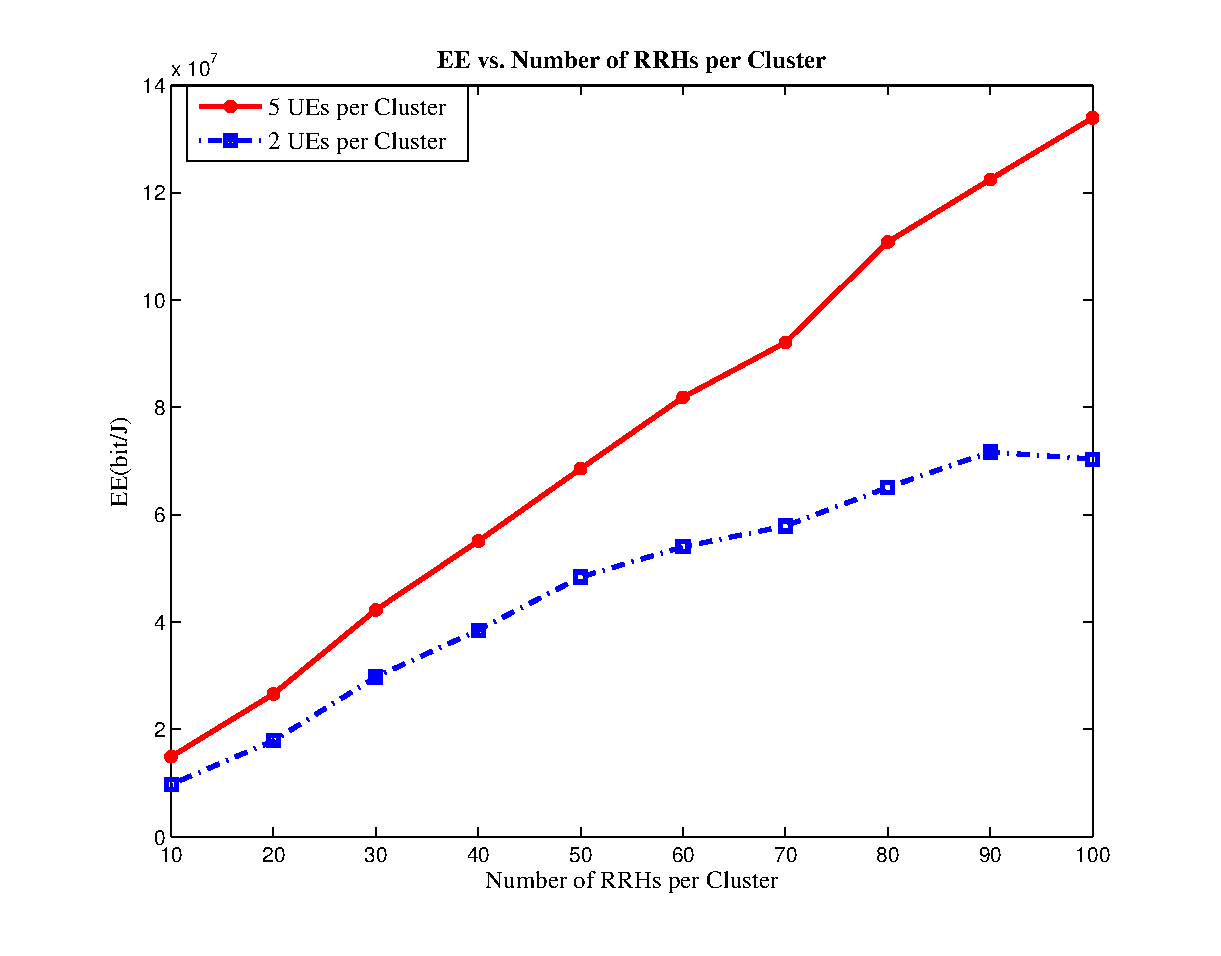
\includegraphics[width=\linewidth, height=12cm]{./fig3/rrh1}
  \caption{
  بازدهی انرژی با توجه به تغییرات تعداد واحدهای رادیویی  در هر خوشه برای توان بهینه برای 
   دو کاربر مختلف
   و پارامترهای جدول \ref{tab:title22}}
  \label{fig:nem1}
\end{figure}
 در شکل \ref{fig:nem1}، بازدهی انرژی سیستم \lr{MIMO C-RAN} بر اساس تعداد واحدهای رادیویی در هر خوشه برای مدل سیستم مورد نظر و برای دو تعداد کاربر متفاوت، رسم شده است. فرض اینجا بر این است که 2 خوشه برای لینک فروسو و دو خوشه برای فراسو وجود دارد.
 همانطور که  شکل  نشان می دهد، با افزایش تعداد واحدهای رادیوی، بازدهی انرژی افزایش می یابد زیرا  در اینجا با افزایش تعداد واحدهای رادیویی، مجموع توان کل افزایش می یابد در نتیجه نرخ انتقال داده نیز بیشتر می گردد و در نتیجه ی آن، بازدهی انرژی نیز افزایش یافته است. همچنین بازدهی انرژی برای تعداد کاربر بیشتر، به دلیل اینکه مجموع نرخ ها بیشتر می گردد، زیادتر می باشد.
 \begin{figure}[H]
  \centering
    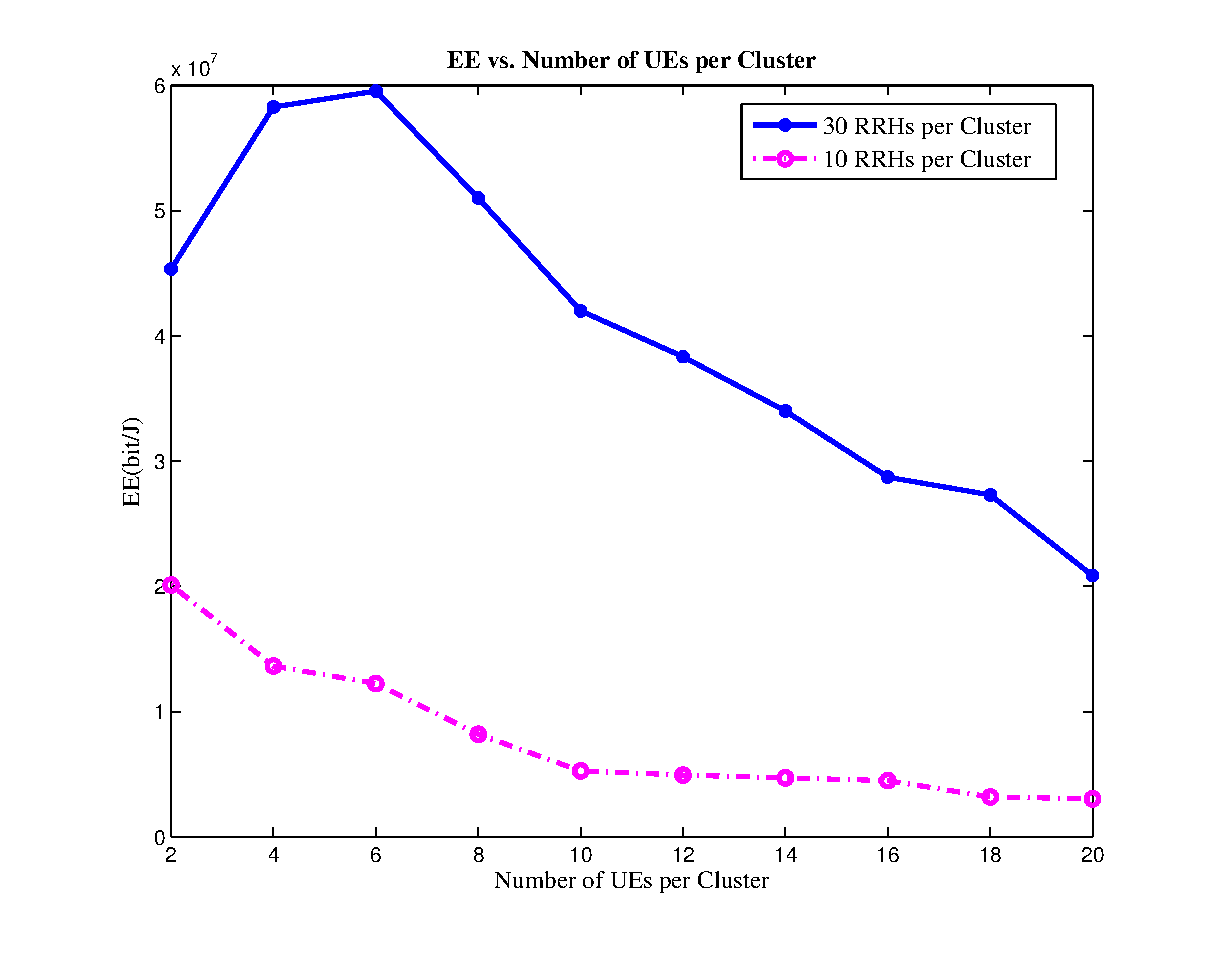
\includegraphics[width=\linewidth]{./fig3/ue4}
  \caption{  بازدهی انرژی با توجه به تغییرات تعداد کاربران در هر خوشه برای توان بهینه برای 
   دو واحد رادیویی مختلف
   و پارامترهای جدول
    \ref{tab:title22} }
  \label{fig:ue4}
\end{figure}

در شکل \ref{fig:ue4}، بازدهی انرژی بر اساس تعداد کاربران در هر خوشه برای مدل سیستم مورد نظر و برای دو تعداد واحد رادیویی متفاوت، رسم شده است. همانطور که  دیده می شود با افزایش تعداد کاربران، در حالتی که 30 واحد رادیویی در هر خوشه داریم، ابتدا به دلیل افزایش کاربران و افزایش مجموع نرخ ها، بازدهی انرژی زیاد شده و در نتیجه ی آن شیب نمودار زیاد می شود ولی از یک مقدار به بعد تداخل بین کاربران افزایش می یابد و منجر به کاهش بازدهی انرژی می گردد. زمانی که تعداد کاربران زیاد نیست، تداخل بین کاربران تاثیر کمی می گذارد و با افزایش کاربران بازدهی انرژی بهبود می یابد ولی زمانی که تعداد کاربران از حدی بیشتر می شود، میزان تداخل به قدری زیاد شده که نرخ انتقال داده کاهش یافته و در نتیجه ی آن، بازدهی انرژی کاهش می یابد. 
در حالتی که  10 واحد رادیویی در هر خوشه داریم، به دلیل اینکه میزان تداخل بین کاربران زیاد است و \lr{SINR} کم است، شیب نمودار از ابتدا منفی است و بازدهی انرژی کم می گردد.
 \begin{figure}[H]
  \centering
    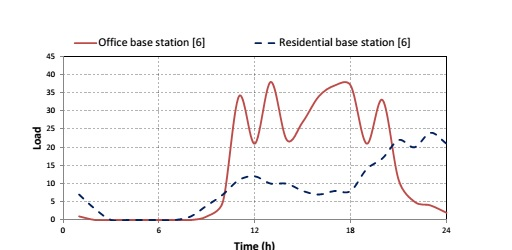
\includegraphics[width=\linewidth]{./fig3/c4}
  \caption{  
  بازدهی انرژی با توجه به تغییرات ظرفیت
   بیشینه ی لینک \lr{fronthaul}
   در هر خوشه برای توان بهینه برای 
   دو تعدا کاربر مختلف
   و پارامترهای جدول
    \ref{tab:title22} }
  \label{fig:c4}
\end{figure}
در شکل \ref{fig:c4}، بازدهی انرژی بر اساس تغییرات ظرفیت
   بیشینه ی لینک \lr{fronthaul} در هر خوشه برای مدل سیستم مورد نظر و برای دو تعداد کاربر متفاوت، رسم شده است.همانطور که  دیده می شود با افزایش این ظرفیت، بازدهی انرژی با شیب زیادی، افزایش یافته ولی از جایی به بعد شیب افزایش کم می گردد زیرا با افزایش بیشینه ی ظرفیت، تعداد بیت های بیشتری می تواند از این لینک عبور کند ولی از یک جایی به بعد، تعداد بیتهایی که در هر ثانیه وجود دارد از نرخ انتقال بیت کمتر است، پس با افزایش نرخ، بازدهی انرژی افزایش پیدا نمی کند. 
\section{نتیجه گیری}
در این فصل، مدل سیستم جدیدی که همزمان شامل چندین خوشه ی لینک فروسو و فراسو است، بیان شده است و همزمان مجموع نرخ های قابل دسترسی بر روی توان کل خوشه های لینک فراسو و فروسو بیشینه شده است و نمودارهای آن را بر حسب تعداد کاربران و واحدهای رادیویی رسم شده اند. با توجه به نمودارها، با افزایش تعداد واحدهای رادیویی توان ارسالی افزایش یافته و بازدهی انرژی بهبود می یابد.  همچنین با افزایش کاربران ابتدا بازدهی انرژی بهبود یافته زیرا مجموع توان افزایش می یابد ولی از حدی به بعد، تاثیر تداخل بین کاربران زیاد شده و بازدهی کاهش می یابد.
		% فصل چهارم: نتایج
% !TeX root=../main.tex
\chapter{بحث و نتیجه‌گیری}
%\thispagestyle{empty} 
\section{مقدمه}
تاکنون شما در پایان‌نامه‌ای که مشغول نوشتن آن هستید، پاسخ چهار سؤال را داده‌اید:
\begin{itemize}
	\item
	چرا تحقیق را انجام دادید؟ (مقدمه)
	\item
	دیگران در این زمینه‌ چه کارهایی کرده‌اند و تمایز کار شما با آنها؟ (مرور ادبیات)
	\item
	چگونه تحقیق را انجام دادید؟ (روش‌ها)
	\item
	چه از تحقیق به دست آوردید؟ (یافته‌ها)
\end{itemize}
حال زمان آن فرا رسیده که با توجه به تمامی مطالب ذکر شده، در نهایت به سؤال آخر پاسخ دهید:
\begin{itemize}
	\item
	چه برداشتی از یافته‌های تحقیق کردید؟ (نتیجه‌گیری)
\end{itemize}
در واقع در این بخش، هدف، پاسخ به این سوال است که چه برداشتی از یافته‌ها کردید و این یافته‌ها چه فایده‌ای دارند؟

نتیجه‌گیری مختصری بنویسید. ارائهٔ داده‌ها، نتایج و یافته‌ها در فصل چهارم ارائه می‌شود. در این فصل تفاوت، تضاد یا تطابق بین نتایج تحقیق با نتایج دیگر محققان باید ذکر شود.
\emph{تفسیر و تحلیل نتایج نباید بر اساس حدس و گمان باشد}،
بلکه باید
\textbf{برمبنای نتایج عملی استخراج‌شده}
از تحقیق و یا
\textbf{استناد به تحقیقات دیگران}
باشد.
با توجه به حجم و ماهیت تحقیق و با صلاحدید استاد راهنما، این فصل می‌تواند تحت عنوانی دیگر بیاید یا به دو فصل جداگانه با عناوین مناسب، تفکیک شود. این فصل فقط باید به جمع‌بندی دست‌آوردهای فصل‌های سوم و چهارم محدود و از ذکر موارد جدید در آن خودداری شود. در عنوان این فصل، به جای کلمهٔ «تفسیر» می‌توان از واژگان «بحث» و «تحلیل» هم استفاده کرد. این فصل شاید مهم‌ترین فصل پایان‌نامه باشد.

در این فصل خلاصه‌ای از یافته‌های تحقیق جاری ارائه می‌شود. این فصل می‌تواند حاوی یک مقدمه، شامل مروری اجمالی بر مراحل انجام تحقیق باشد (حدود یک صفحه). مطالب پاراگراف‌بندی شود و هر پاراگراف به یک موضوع مستقل اختصاص یابد. فقط به ارائهٔ یافته‌ها و دست‌آوردها بسنده شود و
\emph{از تعمیم بی‌مورد نتایج خودداری شود.}
تا حد امکان از ارائهٔ 
\emph{جداول و نمودارها در این فصل اجتناب شود.}
از ارائهٔ 
\emph{عناوین کلی}
در حوزهٔ تحقیق و قسمت پیشنهاد تحقیقات آتی خودداری شود و کاملاً در چارچوب و زمینهٔ مربوط به تحقیق جاری باشد. این فصل حدود ۱۰-۱۵ صفحه است.

\section{محتوا}
به ترتیب شامل موارد زیر است:

\subsection{جمع‌بندی}
خلاصه‌ای از تمام یافته‌ها و دست‌آوردهای تحقیق جاری است.

\subsection{نوآوری}
این قسمت، نوآوری تحقیق را بر اساس یافته‌های آن تشریح می‌کند. که دارای دو بخش اصلی است:
\begin{enumerate}
	\item
	نوآوری تئوری، یعنی تمایز تئوریک کار با کارهای محققین قبلی.
	\item
	نوآوری عملی، یعنی توصیه‌های محقق به صنعت برای بهبود بخشیدن به کارها، بر اساس یافته‌های تحقیق.
\end{enumerate}

\subsection{پیشنهادها}
این بخش، عناوین و موضوعات پیشنهادی را برای تحقیقات آتی،
\emph{بیشتر در زمینهٔ مورد بحث در آینده}
ارائه می‌کند.

\subsection{محدودیت‌ها}
در اینجا انواع محدودیت‌های تحقیق تشریح می‌شوند؛ از جمله، محدودیت‌هایی که کنترل آن از عهده محقق خارج است، مانند انتخاب نوع یافته‌ها؛ و همچنین دیگر محدودیت‌هایی که کنترل آن در دست محقق است، مانند موضوع و محل تحقیق و ... . تأثیر این محدودیت‌ها بر یافته‌های تحقیق در این قسمت شرح داده می‌شوند.		% فصل پنجم: بحث و نتیجه‌گیری

% مراجع
% اگر از استیل‌های natbib استفاده می‌کنید باید دو خط را در فایل commands.tex تغییر دهید.
\pagestyle{empty}
{
\small
\onehalfspacing
%\bibliographystyle{plain-fa} % or plainnat-fa for author-date


\begin{latin}
\bibliographystyle{IEEEtran}
\renewcommand{\bibname}{\rl{{کتاب‌نامه}\hfill}} 
\bibliography{./tex/MyReferences}
\end{latin}
}

\pagestyle{fancy}

% \appendix
% فصلهای پس از این قسمت به عنوان ضمیمه خواهند آمد.

% دستورات لازم برای تبدیل «فصل آ» به «پیوست آ» در فهرست مطالب
\addtocontents{toc}{
    \protect\renewcommand\protect\cftchappresnum{\appendixname~}%
    \protect\setlength{\cftchapnumwidth}{\mylenapp}}
    
\let\Chapter\chapter
% دستورات لازم برای شماره‌گذاری صفحات پیوست‌ها بشکل آ-۱ (فعلا با glossaries سازگار نیست)
%\pretocmd{\chapter}{
%  \clearpage
%  \pagenumbering{arabic}
%  \renewcommand*{\thepage}{\rl{\thechapter-\arabic{page}}}}{}{}
%%%%%%%%%%%%%%%%%%%%%%%%%%%%%%%%%%%%%
    

\chapter*{‌پیوست}
موضوعات مرتبط با متن گزارش پایان نامه كه در يكی از گروه‌های زير قرار می‌گيرد، در بخش پيوست‌ها آورده شوند:
\begin{enumerate}
\item  اثبات های رياضی يا عمليات رياضی طولانی‌.‌
\item داده و اطلاعات نمونه (های) مورد مطالعه (\lr{Case Study}) چنانچه طولانی باشد‌.‌
\item نتايج كارهای ديگران چنانچه نياز به تفصيل باشد‌.‌

\item مجموعه تعاريف متغيرها و پارامترها، چنانچه طولانی بوده و در متن به انجام نرسيده باشد‌.‌
\end{enumerate}
% براي شماره‌گذاري روابط، جداول و اشكال موجود در پيوست‌ از ساختار متفاوتي نسبت به متن اصلي استفاده مي‌شود كه در زير به‌عنوان نمونه نمايش داده شده‌است. 
% \begin{equation}
%F=ma
%\end{equation}
\section*{کد میپل }
\begin{latin}
\begin{verbatim}

with(DifferentialGeometry):
with(Tensor):
DGsetup([x, y, z], M)
																	frame name: M
a := evalDG(D_x)
																	D_x
b := evalDG(-2 y z D_x+2 x D_y/z^3-D_z/z^2)


\end{verbatim}
\end{latin}		% پیوست اول: آشنایی مقدماتی با لاتک
% !TeX root=../main.tex

\chapter{‌جدول، نمودار و الگوریتم در لاتک}
\label{app:latex:more}
%\thispagestyle{empty}

در این بخش نمونه مثالهایی از جدول، شکل، نمودار، الگوریتم و معادلات ریاضی را در لاتک خواهیم دید.
دقت کنید که در پایان‌نامه‌ها و مقالات، باید قاعدهٔ «ارجاع به جلو%
\LTRfootnote{Forward Referencing}»
رعایت شود؛ یعنی ابتدا در متن به شمارهٔ شکل، جدول یا معادله اشاره شود و بعد از آن (زیر آن) خود شکل، جدول یا معادله رسم شود. (توضیحات بیشتر در قسمت
\ref{sec:floatObjs}).

\section{جدول}
دستور اصلی برای رسم جدول در لاتک 
\verb|tabular|
می‌باشد که جدول
\eqref{tab:motionModels}
با استفاده از آن کشیده شده است؛ در
\verb|tabular|
عرض جدول برابر با مجموع عرض ستون‌ها و حداکثر مساوی عرض متن است.
\begin{table}[ht]
\caption{مدلهای تبدیل.}
\label{tab:motionModels}
\centering
\onehalfspacing
\begin{tabular}{|r|c|l|r|}
	\hline نام مدل & درجه آزادی & تبدیل مختصات & توضیح \\ 
	\hline انتقالی & ۲ & $\begin{aligned} x'=x+t_x \\ y'=y+t_y \end{aligned}$  &  انتقال دوبعدی\\ 
	\hline اقلیدسی & ۳ & $\begin{aligned} x'=x\cos\theta - y\sin\theta+t_x \\ y'=x\sin\theta+y\cos\theta+t_y \end{aligned}$  &  انتقالی+دوران \\ 
	\hline 
\end{tabular} 
\end{table}

برای اینکه عرض جدول قابل کنترل باشد، باید از دستورات
\verb|tabularx|،
\verb|tabulary| یا
\verb|tabu|
استفاده کرد که راهنمای آنها در اینترنت وجود دارد.
مثلاً جدول
\ref{tab:motionModelsCont}
با
\verb|tabularx|
رسم شده که عرض جدول در آن ثابت بوده و ستون‌های از نوع
\verb|X|
عرض خالی جدول را پر می‌کنند.
\begin{table}[ht]
	\caption{مدلهای تبدیل دیگر.}
	\label{tab:motionModelsCont}
	\centering
	\onehalfspacing
	\begin{tabularx}{\textwidth}{|r|c|l|X|}
		\hline نام مدل & درجه آزادی & تبدیل مختصات & توضیح \\ 
		\hline مشابهت & ۴ & $\begin{aligned} x'=sx\cos\theta - sy\sin\theta+t_x \\ y'=sx\sin\theta+sy\cos\theta+t_y  \end{aligned}$  & اقلیدسی+تغییرمقیاس \\ 		
		\hline آفین & ۶ & $\begin{aligned} x'=a_{11}x+a_{12}y+t_x \\ y'=a_{21}x+a_{22}y+t_y \end{aligned}$  & مشابهت+اریب‌شدگی \\
		\hline
	\end{tabularx}
\end{table}

\section{معادلات ریاضی و ماتریس‌ها}
تقریباً هر آنچه دانشجویان برای نوشتن فرمول‌های ریاضی لازم دارند، در کتاب 
\lr{mathmode}
آمده است. کافیست در خط فرمان، دستور زیر را وارد کنید:
\begin{latin}
	\texttt{texdoc mathmode}
\end{latin}
متن زیر شامل انواعی از اشیاء ریاضی است که با ملاحظه کدش می‌توانید با دستورات آن آشنا شوید.\\
شناخته‌شده‌ترین روش تخمین ماتریس هوموگرافی الگوریتم تبدیل خطی مستقیم (\lr{DLT\LTRfootnote{Direct Linear Transform}}) است.  فرض کنید چهار زوج نقطهٔ متناظر در دو تصویر در دست هستند،  $\mathbf{x}_i\leftrightarrow\mathbf{x}'_i$   و تبدیل با رابطهٔ
  $\mathbf{x}'_i = H\mathbf{x}_i$
  نشان داده می‌شود که در آن:
\[\mathbf{x}'_i=(x'_i,y'_i,w'_i)^\top  \]
و
\[ H=\left[
\begin{array}{ccc}
h_1 & h_2 & h_3 \\ 
h_4 & h_5 & h_6 \\ 
h_7 & h_8 & h_9
\end{array} 
\right]\]
رابطه زیر را برای الگوریتم  \eqref{alg:DLT} لازم داریم.
\begin{equation}
\label{eq:DLT_Ah}
\left[
\begin{array}{ccc}
	0^\top & -w'_i\mathbf{x}_i^\top & y'_i\mathbf{x}_i^\top \\ 
	w'_i\mathbf{x}_i & 0^\top & -x'_i\mathbf{x}_i^\top \\ 
	- y'_i\mathbf{x}_i^\top & x'_i\mathbf{x}_i^\top & 0^\top
\end{array} 
\right]
\left(
\begin{array}{c}
	\mathbf{h}^1 \\ 
	\mathbf{h}^2 \\ 
	\mathbf{h}^3
\end{array} 
\right)=0
\end{equation}

\section{الگوریتم با دستورات فارسی}
با مفروضات فوق، الگوریتم \lr{DLT} به صورت نشان داده شده در الگوریتم \eqref{alg:DLT}  خواهد بود.
\begin{algorithm}[ht]
\onehalfspacing
\caption{الگوریتم \lr{DLT} برای تخمین ماتریس هوموگرافی.} \label{alg:DLT}
\begin{algorithmic}[1]
\REQUIRE $n\geq4$ زوج نقطهٔ متناظر در دو تصویر 
${\mathbf{x}_i\leftrightarrow\mathbf{x}'_i}$،\\
\ENSURE ماتریس هوموگرافی $H$ به نحوی‌که: 
$\mathbf{x}'_i = H \mathbf{x}_i$.
  \STATE برای هر زوج نقطهٔ متناظر
$\mathbf{x}_i\leftrightarrow\mathbf{x}'_i$ 
ماتریس $\mathbf{A}_i$ را با استفاده از رابطهٔ \ref{eq:DLT_Ah} محاسبه کنید.
  \STATE ماتریس‌های ۹ ستونی  $\mathbf{A}_i$ را در قالب یک ماتریس $\mathbf{A}$ ۹ ستونی ترکیب کنید. 
  \STATE تجزیهٔ مقادیر منفرد \lr{(SVD)}  ماتریس $\mathbf{A}$ را بدست آورید. بردار واحد متناظر با کمترین مقدار منفرد جواب $\mathbf{h}$ خواهد بود.
  \STATE  ماتریس هوموگرافی $H$ با تغییر شکل $\mathbf{h}$ حاصل خواهد شد.
\end{algorithmic}
\end{algorithm}

\section{الگوریتم با دستورات لاتین}
الگوریتم \ref{alg:RANSAC} یک الگوریتم با دستورات لاتین است.

\begin{algorithm}[ht]
\onehalfspacing
\caption{الگوریتم \lr{RANSAC} برای تخمین ماتریس هوموگرافی.} \label{alg:RANSAC}
\begin{latin}
\begin{algorithmic}[1]
\REQUIRE $n\geq4$ putative correspondences, number of estimations, $N$, distance threshold $T_{dist}$.\\
\ENSURE Set of inliers and Homography matrix $H$.
\FOR{$k = 1$ to $N$}
  \STATE Randomly choose 4 correspondence,
  \STATE Check whether these points are colinear, if so, redo the above step
  \STATE Compute the homography $H_{curr}$ by DLT algorithm from the 4 points pairs,
  \STATE $\ldots$ % الگوریتم کامل نیست
  \ENDFOR
  \STATE Refinement: re-estimate H from all the inliers using the DLT algorithm.
\end{algorithmic}
\end{latin}
\end{algorithm}

\section{درج کد}
درج کد به زبان‌های مختلف به سادگی امکان‌پذیر است. برنامه
\ref{code:matlabEx}
یک قطعه کد
\lr{MATLAB}
را نشان می‌دهد.
\singlespacing
\begin{figure}
	\begin{LTR}
		\lstinputlisting[language=MATLAB, caption={نمونه کد \lr{MATLAB}}, label={code:matlabEx}]{MatlabExample.m}
	\end{LTR}
\end{figure}
\doublespacing

\section{تصویر}
نمونهٔ یک تصویر را در فصل قبل دیدیم. دو تصویر شیر کنار هم را نیز در شکل
\ref{fig:twoLion}
مشاهده می‌کنید.
\begin{figure}[ht]
\centering 
\subfloat[شیر ۱]{ \label{fig:twolion:one}

\includegraphics[width=0.3\textwidth]{lion}}
%\hspace{2mm}
\subfloat[شیر ۲]{ \label{fig:twolion:two}

\includegraphics[width=0.3\textwidth]{lion}}%
\caption{دو شیر}
\label{fig:twoLion} %% label for entire figure
\end{figure}

\section{نمودار}
لاتک بسته‌هایی با قابلیت‌های زیاد برای رسم انواع مختلف نمودارها دارد. مانند بسته‌های \lr{Tikz} و  \lr{PSTricks}. توضیح اینها فراتر از این پیوست کوچک است.%
\footnote{
مثال‌هایی از بکارگیری بسته
\lr{Tikz}
را می‌توانید در
\url{http://www.texample.net/tikz/examples/}
ببینید. توصیه می‌شود دانشجویانی که قصد درج اشکالی مانند گراف را در سند خود دارند، مثالهایی از سایت مذکور را ملاحظه فرمایند.
}
یک نمودار رسم شده با بسته‌ی 
\lr{TikZ}
 در شکل 
\ref{fig:parabola}
نشان داده شده است.
\begin{figure}[t]
\centering
\begin{tikzpicture}[scale=2.5]
  \shade[top color=blue,bottom color=gray!50] 
      (0,0) parabola (1.5,2.25) |- (0,0);
  \draw (1.05cm,2pt) node[above] 
      {$\displaystyle\int_0^{3/2} \!\!x^2\mathrm{d}x$};

  \draw[style=help lines] (0,0) grid (3.9,3.9)
       [step=0.25cm]      (1,2) grid +(1,1);

  \draw[->] (-0.2,0) -- (4,0) node[right] {$x$};
  \draw[->] (0,-0.2) -- (0,4) node[above] {$f(x)$};

  \foreach \x/\xtext in {1/1, 1.5/1\frac{1}{2}, 2/2, 3/3}
    \draw[shift={(\x,0)}] (0pt,2pt) -- (0pt,-2pt) node[below] {$\xtext$};

  \foreach \y/\ytext in {1/1, 2/2, 2.25/2\frac{1}{4}, 3/3}
    \draw[shift={(0,\y)}] (2pt,0pt) -- (-2pt,0pt) node[left] {$\ytext$};

  \draw (-.5,.25) parabola bend (0,0) (2,4) node[below right] {$x^2$};
\end{tikzpicture}
\caption{یک نمودار زیبا با ارقام فارسی و قابلیت بزرگ‌نمایی بسیار، بدون از دست دادن کیفیت.}
\label{fig:parabola}
\end{figure}

\section{نحوه قرارگیری اشیای شناور}
\label{sec:floatObjs}
شکل‌ها، جداول و الگوریتم‌ها در لاتک اشیای شناور محسوب می‌شوند؛ یعنی خود لاتک تصمیم می‌گیرد آنها را در کجای صفحه ترسیم کند تا زیباتر باشد. اما می‌توان به لاتک توصیه کرد که آن را در قسمت خاصی از صفحه رسم کند. برای اینکه قاعدهٔ «ارجاع به جلو» رعایت شود باید فقط از پرچم
\verb|[ht]|
استفاده کرد، که می‌گوید اگر جا شد شکل را دقیقاً در همین مکان و در غیراینصورت در بالای صفحه بعد رسم کن.
بنابراین دستورات درج تصویر، جدول و الگوریتم به صورت زیر باید باشند:

\begin{latin}
\begin{verbatim}
	\begin{figure/table/algorithm}[ht]
		...
	\end{figure/table/algorithm}
\end{verbatim}
\end{latin}		% پیوست دوم: جدول، نمودار و الگوریتم در لاتک
% !TeX root=../main.tex
\chapter{مراجع، واژه‌نامه و حاشیه‌نویسی}
\label{app:refMan}
%\thispagestyle{empty}

\section{مراجع و نقل‌قول‌ها}
\label{sec:refUsage}
منابعِ پایان‌نامه، پایه و اساس تحقیق شما به حساب می‌آیند و ضرورت انجام مطالعه و روش‌های به کار رفته در بسیاری از قسمت‌های آن، به کمک منابع صورت می‌گیرد. در استفاده از مراجع علمی در پایان‌نامه، باید سعی کنید بیشتر از
\textbf{منابع چاپ‌شده و مهم}
استفاده کنید و
\emph{ارجاع به داده‌های چاپ نشده، خلاصه‌ها و پایان‌نامه‌ها، سبب به‌هم‌خوردگی و کاهش اعتبار قسمت ارجاع منابع می‌شود.}
استفاده از منابع و نقل قول‌هایی به تحقیق شما ارزش می‌دهند که
\textbf{در راستای هدف تحقیق بوده و به آن اعتبار ببخشند.}
برخی از دانش‌جویان تصوّر می‌کنند که کثرت نقل‌قول‌ها و ارجاعات زیاد، مهم‌ترین معیار علمی شدن پایان‌نامه است؛ حال آنکه استناد به تعداد کثیری از منابع بدون مطالعه دقیق آنها و استفادهٔ مستقیم در پایان‌نامه، می‌تواند نشان‌دهندهٔ عدم احساس امنیت نویسنده باشد!

دو روش برای استفاده از نتایج، جملات، داده‌ها و روش‌های دیگران وجود دارد. یکی نقل‌قول مستقیم و دقیق است و دیگری استفاده غیرمستقیم در متن مقاله، که در ادامه به قواعد این دو نوع نقل‌قول و ارجاع‌دهی اشاره می‌کنیم:
\begin{description}
	\item[نقل‌قول مستقیم:]
	نقل‌قول مستقیم باید دقیق و بدون هیچ تغییری در جملات باشد. بهتر است این‌گونه نقل‌قول‌ها تا حد امکان کوتاه باشد. جملات کوتاه داخل گیومه قرار می‌گیرند و باید به منبع دقیق آن، طبق روش ارجاع‌دهی به منابع، اشاره شود. به عنوان مثال در
	\cite{persianbib87userguide}
	آمده است که:
	\begin{quote}
		«با استفاده از فیلد
		\lr{AUTHORFA}
		می‌توان معادل فارسی نام نویسندگان مقالات لاتین را در متن داشت. معمولاً در اسناد فارسی خواسته می‌شود که پس از ذکر معادل فارسی نام نویسنده، نام لاتین نویسنده(ها) به عنوان پاورقی درج شود
		\citep{persianbib87userguide}.»
	\end{quote}
	\item[نقل‌قول غیرمستقیم:]
	نقل‌قول غیرمستقیم به معنی استفاده از ایده‌ها، نتایج، روش‌ها و داده‌های دیگران در درون متنِ پایان‌نامه، ولی به سبک خودتان و متناسب و هماهنگ با روند پایان‌نامهٔ شماست. در این حالت نیز باید متناسب با شیوهٔ ارجاع‌دهی به آن استناد شود.
\end{description}

با توجه به وجود سبک‌های مختلف ارجاع‌دهی، باید
\textbf{روش قابل قبول و یکسانی}
در طول پایان‌نامه برای اشاره به مراجع در متن و همچنین تهیه فهرست مراجع در انتهای پایان‌نامه بکار رود. مثلاً برای پایان‌نامه‌های مهندسی می‌توان از سبک ارجاع‌دهی
\lr{IEEE}%
\LTRfootnote{\url{http://www.ieee.org/documents/ieeecitationref.pdf}}
یا
\lr{acm}
استفاده کرد. طبیعتاً باید تناظر یک‌به‌یک بین فهرست مراجع در انتهای گزارش و مراجع مورد استفاده در متن باشد%
\footnote{البته گاهی ممکن است محقق مرجعی را مورد مطالعه قرار داده لیکن در متن به آن اشاره نکرده باشد؛ برخی معتقدند در این موارد نیز آوردن آن در فهرست مراجع، اشکالی ندارد، به این شرط که از عنوان «فهرست منابع» به جای «فهرست مراجع» استفاده شود.}.

برای سهولت مدیریت مراجعِ \پ%
، اکیداً توصیه می‌شود از یک ابزار «مدیریت منابع» (با خروجی
\texorpdfstring{\lr{Bib\TeX}}{Bib\TeX}%
) همچون
\lr{Mendeley}،
\lr{Zotero},
\lr{EndNote}
یا
\lr{Citavi}
استفاده کنید.

\subsection{ مدیریت مراجع با  \texorpdfstring{\lr{Bib\TeX}}{Bib\TeX}}
در بخش \ref{Sec:Ref} اشاره شد که با دستور 
 \lr{\textbackslash bibitem}
  می‌توان یک مرجع را تعریف نمود و با فرمان
 \lr{\textbackslash cite}
  به آن ارجاع داد. این روش برای تعداد مراجع زیاد و تغییرات آنها مناسب نیست. برای مدیریت منابع زیاد، سه بستهٔ
\lr{BibTeX} (پیش‌فرض),
\lr{natbib}
(ارجاع‌دهی در متن به صورت نویسنده-سال)
و \lr{BibLaTeX} (جدید و منعطف‌پذیر)
وجود دارند. در ادامه توضیحاتی در مورد مدیریت منابع با \lr{BibTeX} و \lr{natbib} در زی‌پرشین خواهیم آورد که همراه با توزیع‌های معروف تِک عرضه می‌شوند
\footnote{روش \lr{BibLaTeX} هنوز برای متون فارسی به درستی ترجمه نشده است.}.

یکی از روش‌های قدرتمند و انعطاف‌پذیر برای نوشتن مراجعِ مقالات و مدیریت مراجع در لاتک، استفاده از  \lr{BibTeX} است.
 روش کار با بیب‌تک به این صورت است که مجموعهٔ همهٔ مراجعی را که در \پ استفاده کرده یا خواهیم کرد، 
در پروندهٔ جداگانه‌ای با پسوند
\lr{bib}
نوشته و به آن فایل در سند خودمان به صورت مناسب لینک می‌دهیم.
 کنفرانس‌ها یا مجله‌های گوناگون برای نوشتن مراجع، قالب‌ها یا قراردادهای متفاوتی دارند که به آنها استیل‌های مراجع گفته می‌شود.
 در این حالت به کمک ‌استیل‌های بیب‌تک خواهید توانست تنها با تغییر یک پارامتر در پروندهٔ ورودی خود، مراجع را مطابق قالب موردنظر تنظیم کنید. 
 بیشتر مجلات و کنفرانس‌های معتبر یک فایل سبک
 (\lr{BibTeX Style})
با پسوند \lr{bst} در وب‌گاه خود می‌گذارند که برای همین منظور طراحی شده است.

به جز نوشتن مقالات، این سبک‌ها کمک بسیار خوبی برای تهیهٔ مستندات علمی همچون پایان‌نامه‌هاست که فرد می‌تواند هر قسمت از کارش را که نوشت مراجع مربوطه را به بانک مراجع خود اضافه نماید. با داشتن چنین بانکی از مراجع، وی خواهد توانست به راحتی یک یا چند ارجاع به مراجع و یا یک یا چند بخش را حذف یا اضافه ‌نماید؛ 
مراجع به صورت خودکار مرتب شده و
\textbf{فقط مراجع ارجاع داده شده در قسمت کتاب‌نامه خواهندآمد.}
قالب مراجع به صورت یکدست مطابق سبک داده شده بوده و نیازی نیست که کاربر درگیر قالب‌دهی به مراجع باشد. 

\subsection{سبک‌های مورد تأیید دانشگاه تهران}
طبق «دستورالعمل نگارش و تدوین پایان‌نامه» دانشگاه تهران در
\cite{UTThesisGuide}،
ارجاع در متن می‌تواند مطابق با هر یک از دو الگوی هاروارد یا ونکوور باشد:
\singlespacing
\begin{description}
	\item[سیستم نویسنده-سال (هاروارد):]
	ذکر نام نویسنده و سال نشر در متن. در این الگو مراجع بر اساس حروف الفبا تنظیم می‌گردند.
	\item[سیستم شماره‌دار (ونکوور):]
	ارجاع به مراجع به کمک شماره در متن. در این الگو شماره هر مرجع به ترتیب ظاهر شدن آن در متن در داخل کروشه قرار می‌گیرد. فهرست مراجع نیز بر اساس شماره مرجع (نه حروف الفبا) تنظیم می‌گردد.
\end{description}
\doublespacing

در مدیریت منابع با
\lr{\textbf{BibTeX}}،
ارجاع‌ها در متن تنها به شکل
\textbf{شماره‌دار (ونکوور)}
امکان‌پذیر است، گرچه فهرست مراجع می‌تواند با روش‌های مختلف مرتب شود. اگر بخواهیم ارجاع‌ها در متن به صورت
\textbf{نویسنده-سال (هاروارد)}
باشد باید از بستهٔ
\lr{\textbf{natbib}}\LTRfootnote{Natural Sciences Citations \& References}
و استیل‌های مختلف آن استفاده کنیم.

هنگام استفاده از روش نویسنده-سال نوع پرانتزگذاری‌ها در وسط و انتهای جمله با هم فرق خواهد داشت. به مثال زیر مطابق با دستورالعمل
\cite{UTThesisGuide}
توجه کنید:

\textit{
ابتدا
\cite{Khalighi87xepersian}
بستهٔ زی‌پرشین را برای حروف‌چینی فارسی اختراع کرد. بعدها سبک‌های ارجاع‌دهی فارسی و قالب‌های پایان‌نامه نیز مبتنی بر آن ساخته شد
\citep{persianbib87userguide}.
ارجاع‌دهی به مراجع لاتین نیز در زی‌پرشین امکان‌پذیر است. مثلاً
\citelatin{Gonzalez02book}
یک کتاب انگلیسی است و به راحتی به مقالات انگلیسی نیز می‌توان ارجاع داد
\citeplatin{kim2016integrated}.}

در این مثال، ۴ ارجاع در وسط و انتهای جمله به مراجع فارسی و انگلیسی آمده است. وقتی از سیستم نویسنده-سال استفاده می‌کنید، بهتر است ارجاع‌های آخر جمله کلاً داخل پرانتر بیاید؛ بدین منظور باید به جای
\verb|\cite|
از
\verb|\citep|
استفاده کنید. اما در سیستم شماره‌دار چون تمام ارجاع‌ها داخل کروشه می‌آیند این امر اهمیت ندارد.\\
نمی‌توانید در متن فارسی، اسم لاتین محقق خارجی را بیاورید و برای جلوگیری از ایجاد ابهام، صرف‌نظر از نام لاتین هم مجاز نیست! توصیه می‌شود که نام محقق خارجی در متن با حروف فارسی و در پاورقی اسم تمام نویسندگان به صورت انگلیسی آورده شود. نحوهٔ رعایت این نکته را می‌توانید در کد مثال بالا ببینید.

گرچه در تمپلت ورد
\cite{UTThesisGuide}،
به صراحت ذکر شده که بهتر است برای پایان‌نامه‌های مهندسی از سبک 
\lr{IEEE}
استفاده شود (که از سیستم ونکوور تبعیت می‌کند)، اما ترتیب فهرست مراجع در
\lr{IEEE}
بر اساس ترتیب ارجاع در متن بوده و
\emph{مراجع انگلیسی و فارسی از هم تفکیک نمی‌شوند}
که متضاد با دستورالعمل
\cite{UTThesisGuide}
و نیز متضاد عرف اکثر پایان‌نامه‌های فارسی است.
بنابراین دقیقاً نمی‌توان سبک خاصی را برای مراجع پایان‌نامه‌های دانشگاه تهران اجبار کرد. مهم این است که
\textbf{سبک ارجاع‌دهی در تمام طول یک کتابچه}
(مثلاً پایان‌نامه، مقالات یک مجله یا کل یک کتاب) یکسان باشد. بهتر است
\textbf{بسته به حوزه پایان‌نامه}،
در این مورد با استاد راهنمای خود مشورت کنید.

\subsection{سبک‌های فارسی قابل استفاده در زی‌پرشین}
تعدادی از سبک‌های فارسی بسته
\lr{Persian-bib}%
\footnote{ برای اطلاع بیشتر به راهنمای بستهٔ
\lr{Persian-bib}
مراجعه فرمایید.}
که برای  زی‌پرشین آماده شده‌اند، عبارتند از:

\singlespacing
\begin{itemize}
\item \emph{سبک‌های شماره‌دار}:
	\begin{description}
	\item [unsrt-fa.bst] این سبک متناظر با \lr{unsrt.bst} می‌باشد. مراجع به ترتیب ارجاع در متن ظاهر می‌شوند.
	\item [plain-fa.bst] این سبک متناظر با \lr{plain.bst} می‌باشد. مراجع بر اساس نام‌خانوادگی نویسندگان، به ترتیب صعودی مرتب می‌شوند.
	 همچنین ابتدا مراجع فارسی و سپس مراجع انگلیسی خواهند آمد.
	\item [acm-fa.bst] این سبک متناظر با \lr{acm.bst} می‌باشد. شبیه \lr{plain-fa.bst} است.  قالب مراجع کمی متفاوت است. اسامی نویسندگان انگلیسی با حروف بزرگ انگلیسی نمایش داده می‌شوند. (مراجع مرتب می‌شوند)
	\item [ieeetr-fa.bst] این سبک متناظر با \lr{ieeetr.bst} می‌باشد. (مراجع مرتب نمی‌شوند)
	\end{description}
	
\item \emph{سبک‌های نویسنده-سال}:
	\begin{description}
	\item [plainnat-fa.bst] این سبک متناظر با \lr{plainnat.bst} می‌باشد. نیاز به بستهٔ \lr{natbib} دارد. (مراجع مرتب می‌شوند)
	\item [chicago-fa.bst] این سبک متناظر با \lr{chicago.bst} می‌باشد. نیاز به بستهٔ \lr{natbib} دارد. (مراجع مرتب می‌شوند)
	\item [asa-fa.bst] این سبک متناظر با \lr{asa.bst} می‌باشد. نیاز به بستهٔ \lr{natbib} دارد. (مراجع مرتب می‌شوند)
	\end{description}
\end{itemize}
\doublespacing

با استفاده از استیل‌های فوق می‌توانید به انواع مختلفی از مراجع فارسی و لاتین ارجاع دهید.
به عنوان مثال‌هایی از
\textbf{مراجع انگلیسی}،
مرجع
\cite{Baker02limits}\footnote{چون فیلد \lr{authorfa} برای این مرجع تعریف نشده در سبک نویسنده-سال با حروف لاتین به آن در متن ارجاع می‌شود که غلط است.}
مقالهٔ یک ژورنال، مرجع
\cite{Amintoosi09video}
مقالهٔ یک کنفرانس، مرجع
\citelatin{Gonzalez02book}
یک کتاب، مرجع
\cite{Khalighi07MscThesis}
پایان‌نامهٔ کارشناسی ارشد و مرجع
\citelatin{Borman04thesis}
یک رسالهٔ دکتری می‌باشد.\\
همچنین در میان
\textbf{مراجع فارسی},
مرجع
\cite{Vahedi87}
مقالهٔ یک مجله، مرجع
\cite{Amintoosi87afzayesh}
مقالهٔ یک کنفرانس، مرجع
\cite{Pedram80osool}
یک کتاب ترجمه‌شده با ذکر مترجمان و ویراستاران، مرجع
\cite{Pourmousa88mscThesis}
پایان‌نامهٔ کارشناسی ارشد%
\footnote{همان‌طور که در بخش
\ref{sec:refUsage}
اشاره شد، بهتر است زیاد از پایان‌نامه‌ها در مراجع استفاده نکنید.}،
مرجع
\cite{Omidali82phdThesis}
یک رسالهٔ دکتری و مراجع
\cite{persianbib87userguide, Khalighi87xepersian}
نمونه‌های متفرقه هستند.

\subsection{ساختار فایل مراجع}
برای استفاده از بیب‌تک باید مراجع خود را در یک فایل با پسوند \lr{bib} ذخیره نمایید. یک فایل \lr{bib} در واقع یک پایگاه داده از مراجع%
\LTRfootnote{Bibliography Database}
شماست که هر مرجع در آن به عنوان یک رکورد از این پایگاه داده
با قالبی خاص ذخیره می‌شود. به هر رکورد یک مدخل%
\LTRfootnote{Entry}
گفته می‌شود. یک نمونه مدخل برای معرفی کتاب \lr{Digital Image Processing} در ادامه آمده است:

\singlespacing
\begin{LTR}
\begin{verbatim}
@BOOK{Gonzalez02image,
  AUTHOR     = {Gonzalez,, Rafael C. and Woods,, Richard E.},
  TITLE      = {Digital Image Processing},
  PUBLISHER  = {Prentice-Hall, Inc.},
  YEAR       = {2006},
  ISBN       = {013168728X},
  EDITION    = {3rd},
  ADDRESS    = {Upper Saddle River, NJ, USA}
}
\end{verbatim}
\end{LTR}
\doublespacing

در مثال فوق، \lr{@BOOK} مشخصهٔ شروع یک مدخل مربوط به یک کتاب و \lr{Gonzalez02book} برچسبی است که به این مرجع منتسب شده است.
 این برچسب بایستی یکتا باشد. برای آنکه بتوان
\textbf{برچسب مراجع}
 را به راحتی به خاطر سپرد و حتی‌الامکان برچسب‌ها متفاوت با هم باشند، معمولاً از قوانین خاصی به این منظور استفاده می‌شود. یک قانون می‌تواند
\textbf{فامیل نویسنده اول + دورقم سال نشر + اولین کلمهٔ عنوان اثر}
باشد. به
\lr{AUTHOR}، \lr{TITLE}، $\dots$ و \lr{ADDRESS}
فیلدهای این مدخل گفته می‌شود، که هر یک با مقادیر مربوط به مرجع پر شده‌اند. ترتیب فیلدها مهم نیست. 

انواع متنوعی از مدخل‌ها برای اقسام مختلف مراجع همچون کتاب، مقالهٔ کنفرانس و مقالهٔ ژورنال وجود دارد که برخی فیلدهای آنها با هم متفاوت است. 
نام فیلدها بیانگر نوع اطلاعات آن می‌باشد. مثالهای ذکر شده در فایل \lr{MyReferences.bib} کمک خوبی برای شما خواهد بود. 
%این فایل یک فایل متنی بوده و با ویرایشگرهای معمول همچون \lr{Notepad++} قابل ویرایش می‌باشد. برنامه‌هایی همچون 
%\lr{TeXMaker}
% امکاناتی برای نوشتن این مدخل‌ها دارند و به صورت خودکار فیلدهای مربوطه را در فایل \lr{bib}  شما قرار می‌دهند.  
با استفاده از سبک‌های فارسی آماده شده، محتویات هر فیلد می‌تواند به فارسی نوشته شود؛ ترتیب مراجع و نحوهٔ چینش فیلدهای هر مرجع را سبک مورد استفاده  مشخص خواهد کرد.

\textbf{در فایل 
\lr{MyReferences.bib}
 که همراه با این \پ هست، مثال‌های مختلفی از مراجع آمده‌اند که برای درج مراجع خود، تنها کافیست مراجع‌تان را جایگزین موارد مندرج در آن نمایید.
}

برای بسیاری از مقالات لاتین حتی لازم نیست که مدخل مربوط به آنرا خودتان بنویسید. با جستجوی 
\textbf{نام مقاله + کلمه
\lr{bibtex}}
در اینترنت سایت‌های بسیاری همچون
\lr{ACM} و \lr{ScienceDirect}
را خواهید یافت که مدخل
\lr{bibtex}
مربوط به مقاله شما را دارند و کافیست آنرا به انتهای فایل
\lr{MyReferences.bib}
اضافه کنید.

\subsection{نحوه اجرای \texorpdfstring{\lr{Bib\TeX}}{Bib\TeX}}
پس از قرار دادن مراجع خود، برای ساخت فایل خروجی می‌توانید دستور زیر را (در ترمینال یا از طریق \lr{Texmaker}) اجرا کنید:%
\footnote{فایل \lr{latexmkrc} باید در کنار \lr{main.tex} وجود داشته باشد.}

\singlespacing
\begin{LTR}
	\begin{verbatim}
		latexmk -bibtex -pdf main.tex
	\end{verbatim}
\end{LTR}
\doublespacing
ابزار \lr{latexmk} مراحل مختلف ساخت خروجی لاتک را به طور خودکار و بهینه انجام می‌دهد و هر بار فقط مراحلی را که لازم باشد تکرار می‌کند.
روش دستی‌تر این است که یک بار \lr{XeLaTeX} را روی سند خود اجرا نمایید، سپس \lr{bibtex} و پس از آن هم ۲ بار \lr{XeLaTeX} را. در \lr{TeXMaker} کلید \lr{F11} و در \lr{TeXWorks} هم گزینه‌ی \lr{BibTeX} از منوی \lr{Typeset}، \lr{BibTeX} را روی سند شما اجرا می‌کنند.

\section{واژه‌نامه‌ها و فهرست اختصارات}
\gls{Gloss}
یا فرهنگ لغات، مجموعه‌ای از اصطلاحات و تعاریف خاص و فنی است که معمولاً در انتهای یک کتاب می‌آید. چون پایان‌نامه خود یک متن تخصصی بلند محسوب می‌شود، استفاده از فرهنگ لغات در انتهای آن به شدت توصیه می‌شود، خصوصاً که احتمال استفاده از لغات تخصصی لاتین در آن بالاست.
واژه‌نامه‌هایی که در انتهای کتاب‌های انگلیسی می‌آیند معمولاً تک‌زبانه هستند و معنی یک اصطلاح تخصصی در آنها، عمدتاً به صورت یک
\gls{Description}
طولانی آورده می‌شود. اما چون در متون فارسی، آوردن لغات انگلیسی مجاز نیست و باید معادل فارسی آنها وارد شود، جهت رفع ابهام معمولاً واژه‌نامهٔ فارسی به انگلیسی (و برعکس) در انتهای کتاب درج شده و  
\glspl{Description}
در صورت نیاز در متن آورده می‌شوند.

فهرست
\glspl{Acronym}
شامل نمادهای کوتاهی است که اغلب از حروف ابتدایی کلمات یک عبارت طولانی ساخته شده‌اند. با اینکه
\glspl{Acronym}
با حروف (بزرگ) لاتین نوشته می‌شوند، اما چون کوتاهند استفاده از آنها در میان متن فارسی مجاز است. با این حال برای رفع ابهام، عرف است که فهرستی از آنها شامل معنی هر نماد، در کنار دیگر فهرست‌ها در ابتدای متن درج شود.

در این قالب پایان‌نامه، برای ساخت و مدیریت واژه‌نامه و فهرست اختصارات از بستهٔ پیشرفتهٔ
\lr{glossaries}
با موتور واژه‌نامه‌سازی
\lr{xindy}
استفاده می‌شود. تنظیمات بهینهٔ این بسته در فایل
\lr{glossaries-settings.tex}
عبارتند از:
\begin{itemize}
	\item
قبل از درج واژه‌ها در متن، باید مدخل آنها با دستور زیر (ترجیحاً در فایل جدای \lr{words.tex}) تعریف شود:
	\begin{LTR}
	\verb|\newword{Label}{Word}|\{واژه\}\{واژه‌ها\}
	\end{LTR}
	
	\item
قبل از وارد کردن علائم اختصاری در متن، باید مدخل آنها نیز (ترجیحاً در فایل \lr{acronyms.tex}) به صورت زیر تعریف شود:
	\begin{LTR}
	\verb|\newacronym{Label}{Acr}|\{معنی‌اختصار\}
	\end{LTR}

	\item
جهت درج یک علامت اختصاری یا معادل یک واژه تخصصی، کافی است از دستور
	\verb|gls{Label}|
در متن استفاده کنید. دستور
	\verb|glspl{Label}|
نیز برای آوردن معادل یک لغت در حالت جمع ساخته شده است.
	
	\item
هنگام اولین استفاده از یک معادل فارسی یا اختصار در متن، معادل انگلیسی یا معنی آن در پاورقی آورده می‌شود. در صورتی که هر یک از این پیش‌فرض‌ها را دوست ندارید با ویرایش فایل
	\lr{glossaries-settings.tex}
می‌توانید آن را تغییر دهید.

	\item
در انتهای پایان‌نامه با دستور
\verb|\printglossary|
فهرست کلمات استفاده‌شده به ترتیب الفبای فارسی (واژه‌نامه فارسی به انگلیسی) و الفبای انگلیسی (واژه‌نامه انگلیسی به فارسی) درج می‌شود.
\end{itemize}

به عنوان مثال، با مشاهدهٔ کد این نوشته، نحوهٔ درج معادل فارسی
\gls{RandomVariable}
را در متن مشاهده می‌کنید.
در نمایش واژهٔ
\gls{RandomVariable}
برای بار دوم، معادل لاتین در پاورقی نمی‌آید.
در مورد درج علائم اختصاری، مثلاً می‌توان به رابطهٔ
\gls{F}
اشاره کرد.

\section{حاشیه‌نویسی در نسخه پیش‌نویس}
اصلاح و بازبینی چندین و چندبارهٔ یک پایان‌نامه یا مقاله، از معمول‌ترین امور در نگارش آن می‌باشد. فرض کنید دانشجو پایان‌نامه یا مقالهٔ خود را (کامل یا ناقص) نوشته و می‌خواهد نظر استاد راهنما، اعضای آزمایشگاه یا دیگر متخصصین را در مورد آن جویا شود. به جز مشاورهٔ حضوری، تلفنی یا از طریق ایمیل، برای اظهارنظر دقیق بر نوشته، می‌توان از ابزارهای حاشیه‌نویسی در فایل
\lr{PDF}
یا \lr{tex}
نیز استفاده کرد.

یک راهکار مناسب برای حاشیه‌نویسی در فایل \lr{tex}، استفاده از بسته 
\lr{todonotes}
می‌باشد که آقای خلیقی به تازگی امکان استفاده از آن را برای فارسی‌زبانان نیز فراهم آورده‌اند.
بدین منظور، هر جایی که خواستید نکته یا نکاتی را در حاشیه متن یادداشت کنید، کافی است دستور زیر را وارد نمایید:
\begin{latin}
\verb|\todo{NOTE}|
\end{latin}
مثلاً استاد راهنما می‌تواند از دانشجو بخواهد که در بخشی توضیح بیشتری دهد.
\todo{
توضیح بیشتری لازم است.
}
استاد راهنما یا داور حتی می‌تواند محل پیشنهادی برای درج یک تصویر را نیز به راحتی برای دانشجو مشخص کند.
\missingfigure[figwidth=\textwidth,figcolor=white]{یک تصویر از خروجی الگوریتم 
\ref{alg:RANSAC}
را در اینجا قرار دهید.}
یکی دیگر از امکانات این بسته آن است که می‌توان فهرست نکات را در ابتدای سند داشت. بسته 
\lr{todonotes}
امکانات بسیاری دارد
\todo[fancyline,color=green!30]{مرجع این مطلب؟}
که در راهنمای آن معرفی شده است و با اجرای دستور زیر در خط فرمان می‌توانید آنها را مشاهده کنید:
\begin{latin}	
	\texttt{texdoc todonotes}
\end{latin}	
دقت کنید که توضیحات حاشیه‌ای و فهرست کارهای باقیمانده (نکات)،
\textbf{فقط در نسخه
\gls{Draft}}
قابل دیدن هستند و در نسخه نهایی، نمایش داده نخواهند شد.
برای استفاده از حالت
\gls{Draft}
باید گزینه 
\lr{draft}
به دستور 
\verb|\documentclass|
در ابتدای فایل 
\lr{main.tex}
اضافه شود.
هنگامی‌که سند شما در حالت 
\gls{Draft}
باشد:

\singlespacing
\begin{enumerate}
\item 
هیچ یک از صفحات آغازین پایان‌نامه، تا فهرست مطالب نمایش داده نمی‌شود (به جز صفحه اول).
\item
روی صفحه اول عبارت «پیش‌نویس» به صورت درشت و کم‌رنگ نمایش داده می‌شود.
\item
فهرست نکات درج شده توسط
\lr{todo}،
پس از فهرست اصلی و با عنوان «فهرست کارهای باقیمانده» نمایش داده می‌شود.
\item
شماره صفحاتی که به هر مرجع ارجاع داده شده است در بخش مراجع نمایش داده می‌شود
\footnote{اعمال گزینهٔ
\lr{pagebackref}
برای بستهٔ
\lr{hyperref}.
}.
\end{enumerate}
\doublespacing
هر یک از موارد بالا تا زمانی که نسخه نهایی \پ نیاز نباشد بسیار مورد توجه و مفید واقع می‌شوند.
   	% پیوست سوم: مراجع، واژه‌نامه و حاشیه‌نویسی

% برگرداندن شماره‌بندی صفحات فصول
\let\chapter\Chapter
\pagenumbering{tartibi} % اول، دوم، ...
%\baselineskip=.75cm

% چاپ واژه‌نامه‌ها و نمایه 
\onehalfspacing
\printglossary
\printindex

\begin{latin}
\baselineskip=.6cm
\latinTitlePage
\end{latin}
\label{LastPage}

\end{document}